% %
% LAYOUT_E.TEX - Short description of REFMAN.CLS
% 99-03-20
%
% Updated for REFMAN.CLS (LaTeX2e)
%
\documentclass[twoside,letterpaper]{refart}
\usepackage{makeidx}
\usepackage{ifthen}
\usepackage{enumitem}
\usepackage{gensymb}
\usepackage{textcomp}
\usepackage{todo}
\usepackage{graphicx}
%\usepackage{placeins}
\usepackage[section]{placeins}
\usepackage{hyperref}
\usepackage{booktabs}
\usepackage[dvipsnames]{xcolor}
\usepackage{amsmath}
\usepackage{tikz}
\usepackage{pgf}
\hypersetup{
	colorlinks=true,
	linkcolor={CadetBlue},
	filecolor=magenta,
	urlcolor={CadetBlue}
	}

\urlstyle{same}

\graphicspath{ {images/} }
% ifthen wird vom Bild von N.Beebe gebraucht!

\def \bs{\char'134 } % backslash in \tt font.
\newcommand{\ie}{i.\,e.,}
\newcommand{\eg}{e.\,g..}
\DeclareRobustCommand \cs[1]{\texttt{\char`\\#1}}
\DeclareUnicodeCharacter{2212}{-} % add unicode minus sign 

\title{Photosensor Test Facility Operations Manual}
\author{TRIUMF National Laboratory \\
Alexander Jaffray \\
Kevin Xie \\
Mia Kramer \\
Skylar Wingfelder\\
% {\today} \\
Version 5}

\date{Updated \today}
\emergencystretch1em %

% controls the width of the pictures included in figures
\newcommand{\picwidth}{0.7 \textwidth}

\pagestyle{myfootings}
\markboth{Operations Manual: Photosensor Test Facility}%
         {Operations Manual: Photosensor Test Facility}

\makeindex

\setcounter{tocdepth}{2}

\begin{document}

\maketitle

\begin{abstract}
	This document describes standard operation of the Photosensor Test Facility (PTF) at TRIUMF, and is intended to be a "living" document, added to as functionality is implemented.
\end{abstract}
\tableofcontents

\newpage


%%%%%%%%%%%%%%%%%%%%%%%%%%%%%%%%%%%%%%%%%%%%%%%%%%%%%%%%%%%%%%%%%%%%

\section{Introduction}

The Photosensor Test Facility at TRIUMF is an experiment set up to accurately test and characterize the behaviour of photosensors (for use in large High Energy Physics experiments, including the existing Super-Kamiokande neutrino observatory and the forthcoming Hyper-Kamiokande megaton scale neutrino detector). These detectors utilize photomultiplier tubes as a means of detecting Cherenkov light from neutrino interactions. Specifically, the Super-K detector contains $11,000$ such photomultiplier tubes and the Hyper-K detector would contain up to $90,000$ photomultiplier tubes in two water tanks. As such, it is necessary to measure the individual response of these PMTs to various conditions in order to more accurately simulate, model and understand the large-scale behaviour of the detectors and the data that they collect. The PTF is designed to measure 20 inch PMTs but is capable of measuring the response of wide range of other size tubes.

\subsection{Required Knowledge and Notes}

Operation of the Photosensor Test Facility at TRIUMF requires familiarity with basic electronics concepts such as current, voltage, and resistance. Familiarity with the photoelectric effect and basic physics, as well as working knowledge of the Python, C and C++ programming languages and the ROOT analysis package is very beneficial, but not required.

CSA approved safety footwear with a steel toe is required in the Meson Hall. A stipend from TRIUMF is available to aid this purchase if necessary. All other safety equipment, such as hard hats, face shields, gloves and jacket will be provided in the PTF.



\subsection{Contact and Help}

If there is any additional assistance/guidance required, please do not hesitate to contact Thomas Lindner. Their offices are in Trailer Ff and emails are available at the TRIUMF staff directory website. Thomas' building is at ISAC-II.\@ As well, the TRIUMF main control room number is 7333.

\begin{center}\begin{tabular}{rl}
	Thomas Lindner & lindner@triumf.ca \\
	John Walker    & jmgwalker@triumf.ca \\
	Patrick de Perio     & pdeperio@triumf.ca
\end{tabular}\end{center}

\newpage

\section{Getting Started}

\subsection{Finding the PTF}

The PTF is located on the first floor of the Meson Hall Extension Service Annex. Directions to the PTF from the Badge Room are as follows:

\begin{enumerate}
	\item Upon exiting the Badge Room, turn left and walk towards ISAC 1
	\item Enter the Meson Hall loading bay (on the right), either through the main bay doors or through the small access door on the right side adjacent to the compressed gas tanks
	\item Once inside the Meson Hall, turn left towards the helium recovery area and walk down the hallway
	\item Proceed down the short stairs by the scissor lift, make a right around the clean room and walk to the Meson Hall Extension Service Annex 
	\item Once in MHESA, the PTF is the first room on the right.
	\item Check the status screen. If the PMT is on, do not open the curtain, and do not turn on the room lights, use a flashlight when in the room. If the screen indicates that a run is in progress, only enter if really necessary, following the precautions above
\end{enumerate}

\subsection{Accessing the PTF Main Status Page}

Operation of the PTF (with the exception of making mechanical changes to the configuration or performing data analysis) is primarily performed by accessing the webpage hosted on the computer \textbf{midptf01}.

To access the main control webpage, navigate to the following address using a web browser: \href{https://midptf01.triumf.ca}{\texttt{https://midptf01.triumf.ca}}. Note that the http \textbf{s} is important, as \href{http://midptf01.triumf.ca}{\texttt{http://midptf01.triumf.ca}} will take you to the Sentry Switched CDU control page.

When prompted, use \texttt{midptf} as the username, and \texttt{pmtCalib123} as the password.

Upon logging in, a status page will appear, from which all control and operational functionalities of the PTF are accessible.

The main status page shown in Fig. 1 presents the user with a summary of the current status of the PTF and provides access to different functionality and control of the PTF.

\begin{figure}[!htpb]\centering	
	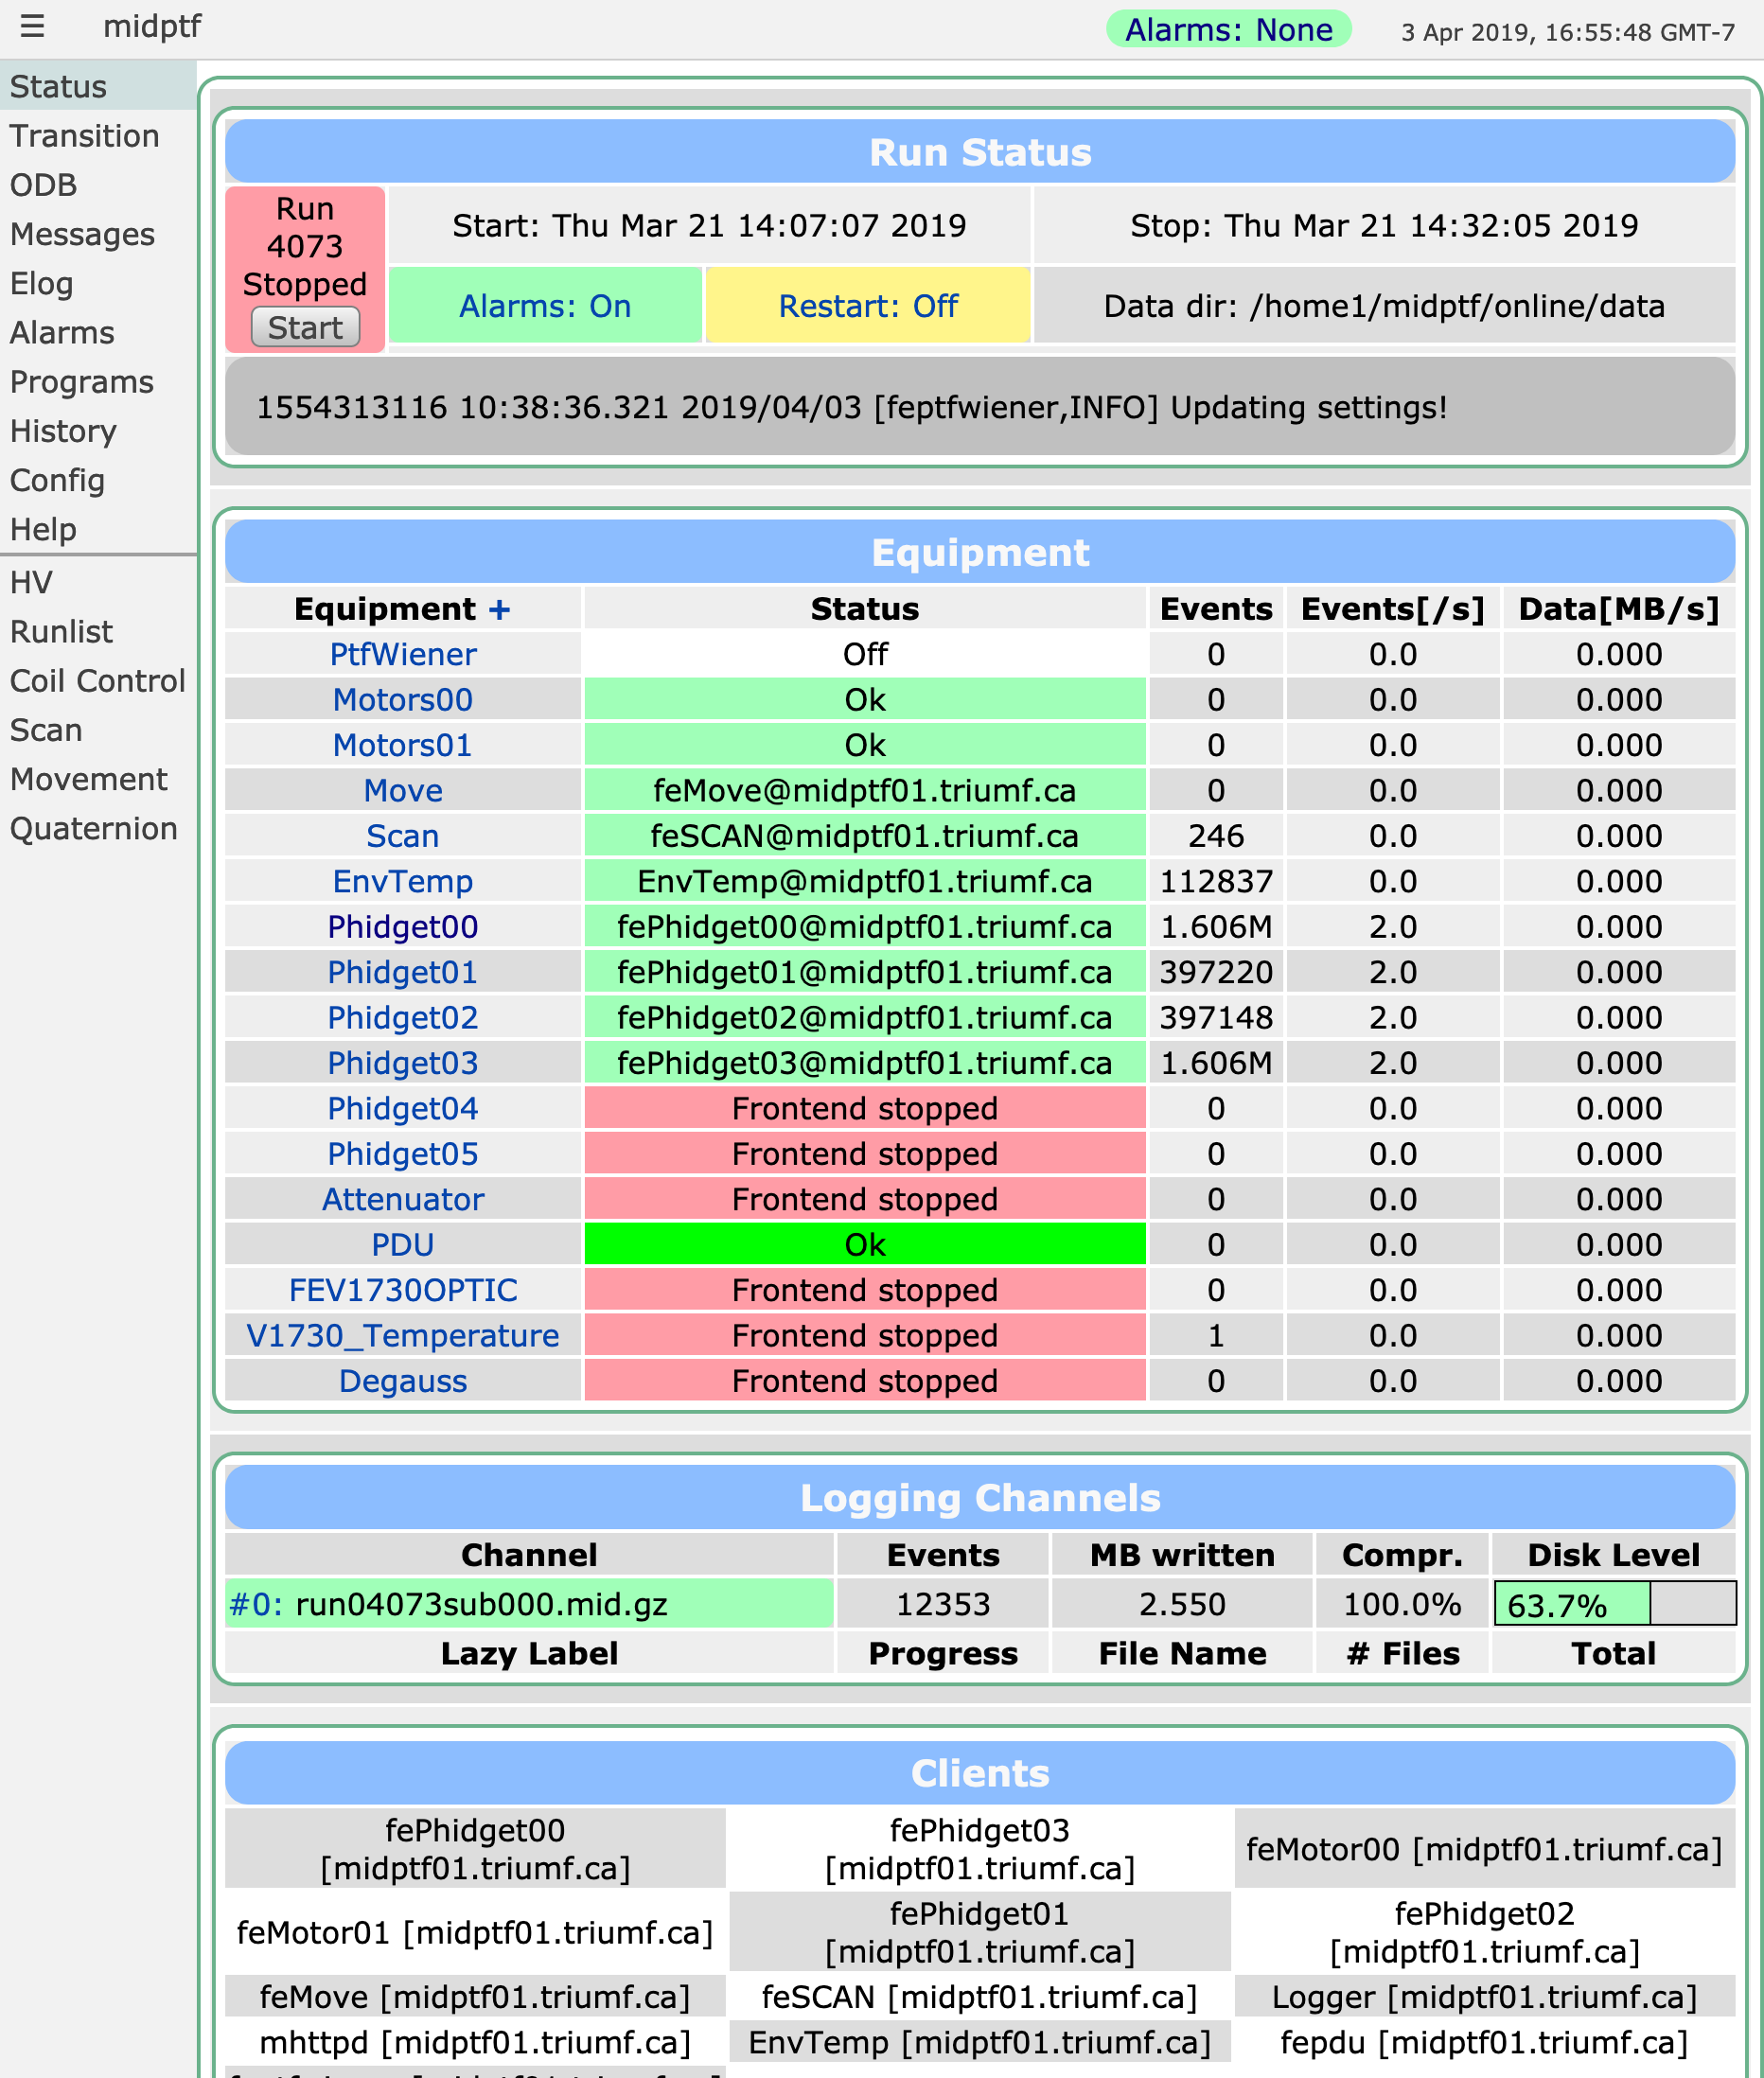
\includegraphics[width=\textwidth]{images/midptfStatusPage.png}
	\caption{Status Page for PTF Operation\label{statusPage}}
\end{figure}

\clearpage

\subsection{Main PTF Status Page}

\subsubsection{Navigation Tabs} The \textbf{Navigation Tabs} on the main status page (small grey text tabs in the page header) allow access to various status, logging and control pages for different pieces of equipment in the PTF.

\FloatBarrier

\begin{figure}[!htpb]\centering	
	
\includegraphics[width=0.15\textwidth]{images/navTabs.png}
	\caption{Navigation Tabs\label{navTabs}}
\end{figure}

\FloatBarrier

\subsubsection{Run Status Section}

The \textbf{Run Status} section of the main status page lists the current or most recently completed measurement run, the duration of the run, the time it was started at, and provides a live feed of control messages from the equipment being used. A Start/Stop button provides the primary means for run control.

\FloatBarrier

\begin{figure}[!htpb]\centering	
	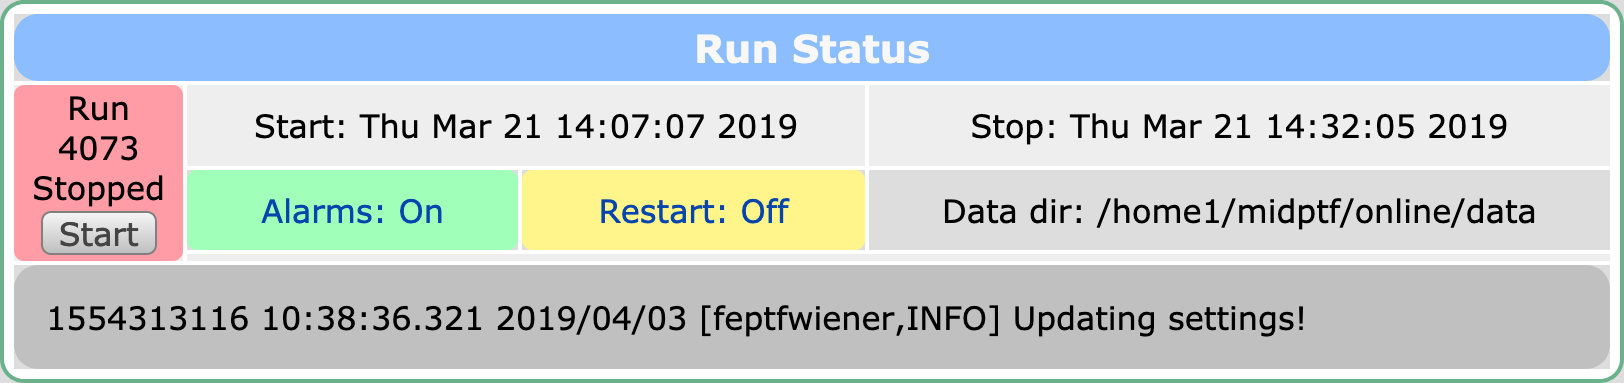
\includegraphics[width=\textwidth]{images/runStatus.png}
	\caption{Run Status Section\label{runStatus}}
\end{figure}

\FloatBarrier

\subsubsection{Equipment}

The \textbf{Equipment} section of the main status page lists the current operational status of all of the equipment in the PTF.\@ A brief description of the equipment can be found in Section~\ref{Terminology}.

\FloatBarrier

\begin{figure}[!htpb]\centering	
	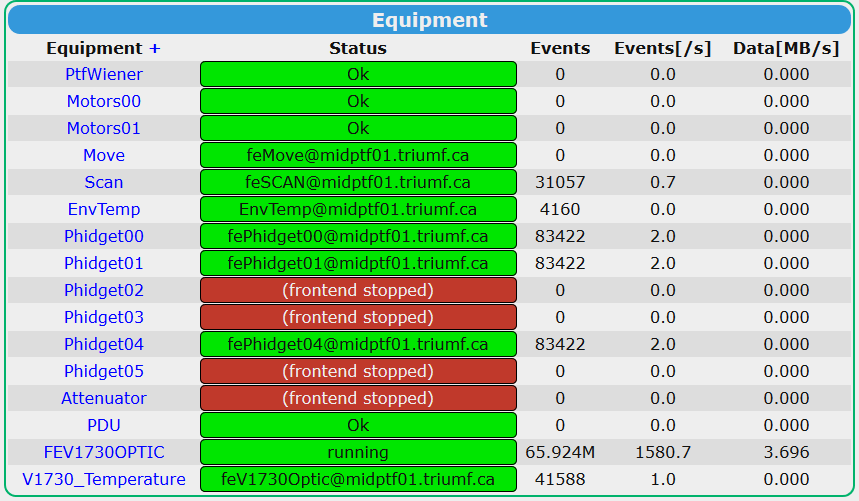
\includegraphics[width=\textwidth]{images/equipment.png}
	\caption{Equipment Section\label{equipment}}
\end{figure}

\FloatBarrier

\subsubsection{Logging Channels}

The \textbf{Logging Channels} section of the main status page lists the status of recorded MIDAS data, including the raw file data name, the amount of data recorded, number of events recorded and compression level of the file. If the text under Channel is in a Yellow or Red Bubble (It is Green in the picture below), then no data will be logged. This must be green to log data for a run. Additionally, the write data option must be checked at the time of run start.

\FloatBarrier

\begin{figure}[!htpb]\centering	
	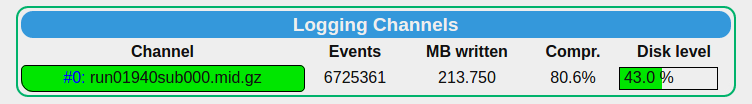
\includegraphics[width=\textwidth]{images/loggingChannels.png}
	\caption{Logging Channels Section\label{loggingChannels}}
\end{figure}

\FloatBarrier

\subsubsection{Clients}

The \textbf{Clients} section of the main status page shows a list of all client programs interfaced with by the status page. This section is mainly for debugging purposes.

\FloatBarrier

\begin{figure}[!htpb]\centering	
	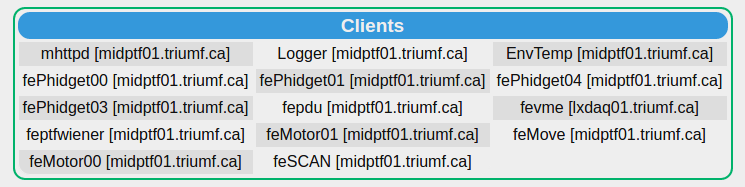
\includegraphics[width=\textwidth]{images/clients.png}
	\caption{Clients Section\label{clients}}
\end{figure}

\FloatBarrier

\clearpage

\subsection{PTF Hardware: Identification and Description}

Operation of the PTF involves the use of a variety of hardware devices which interface to the control systems accessible from the Main Status Page in Section~\ref{statusPage}. The ability to identify and understand each hardware component is beneficial when setting up the system after a configuration change or when troubleshooting. This section details each hardware component and describes its functionality in greater detail than that provided in Section~\ref{Terminology}.

\FloatBarrier

\begin{figure}[!htpb]\centering	
	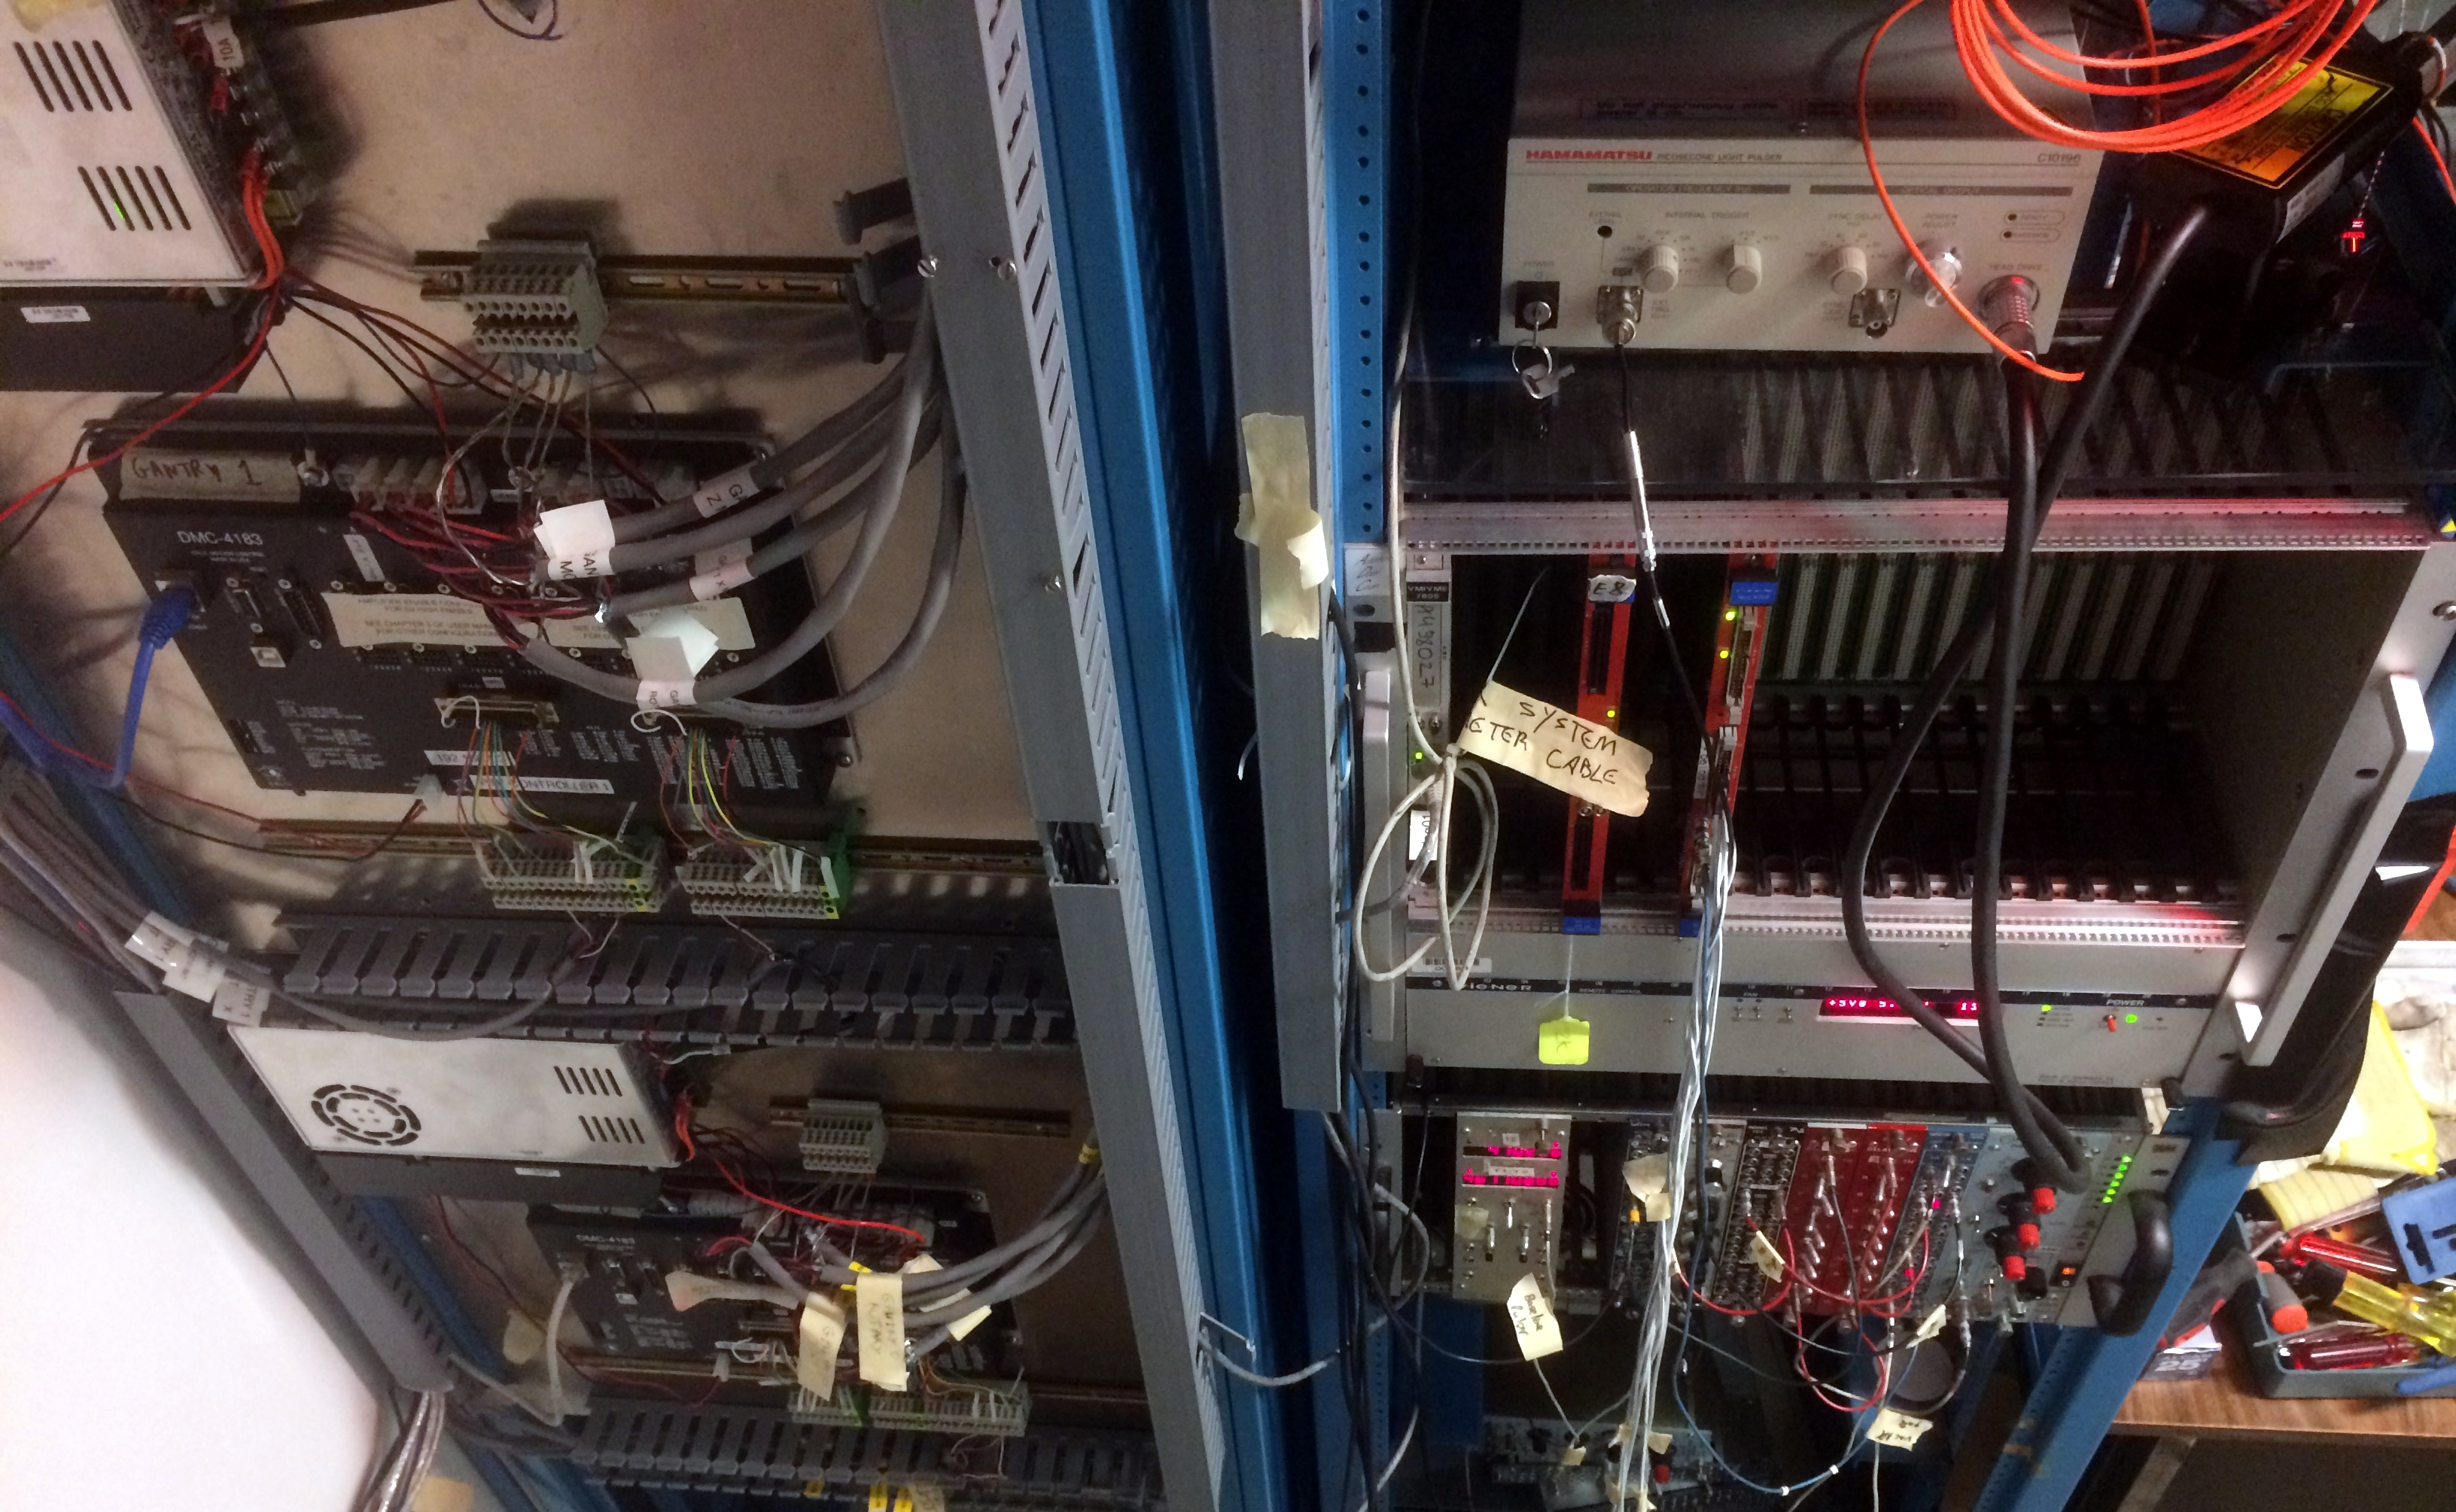
\includegraphics[width=\picwidth]{images/rack}
	\caption{Main Electronics Equipment Rack\label{mainEquipmentRack}}
\end{figure}

\FloatBarrier

\subsubsection{Wiener Crate}

Provides constant voltage output to PMTs and Helmholtz coil system. Power delivery is facilitated by a number of individually controllable channels, of which 11 are in use under normal conditions. Control of this equipment can be accessed either completely through the \textbf{HV Navigation Tab} or partially through the \textbf{Coil Control Navigation Tab}. The Wiener Crate is located in the main equipment rack as shown in Figure~\ref{wiener}.

\FloatBarrier

\begin{figure}[!htpb]\centering	
	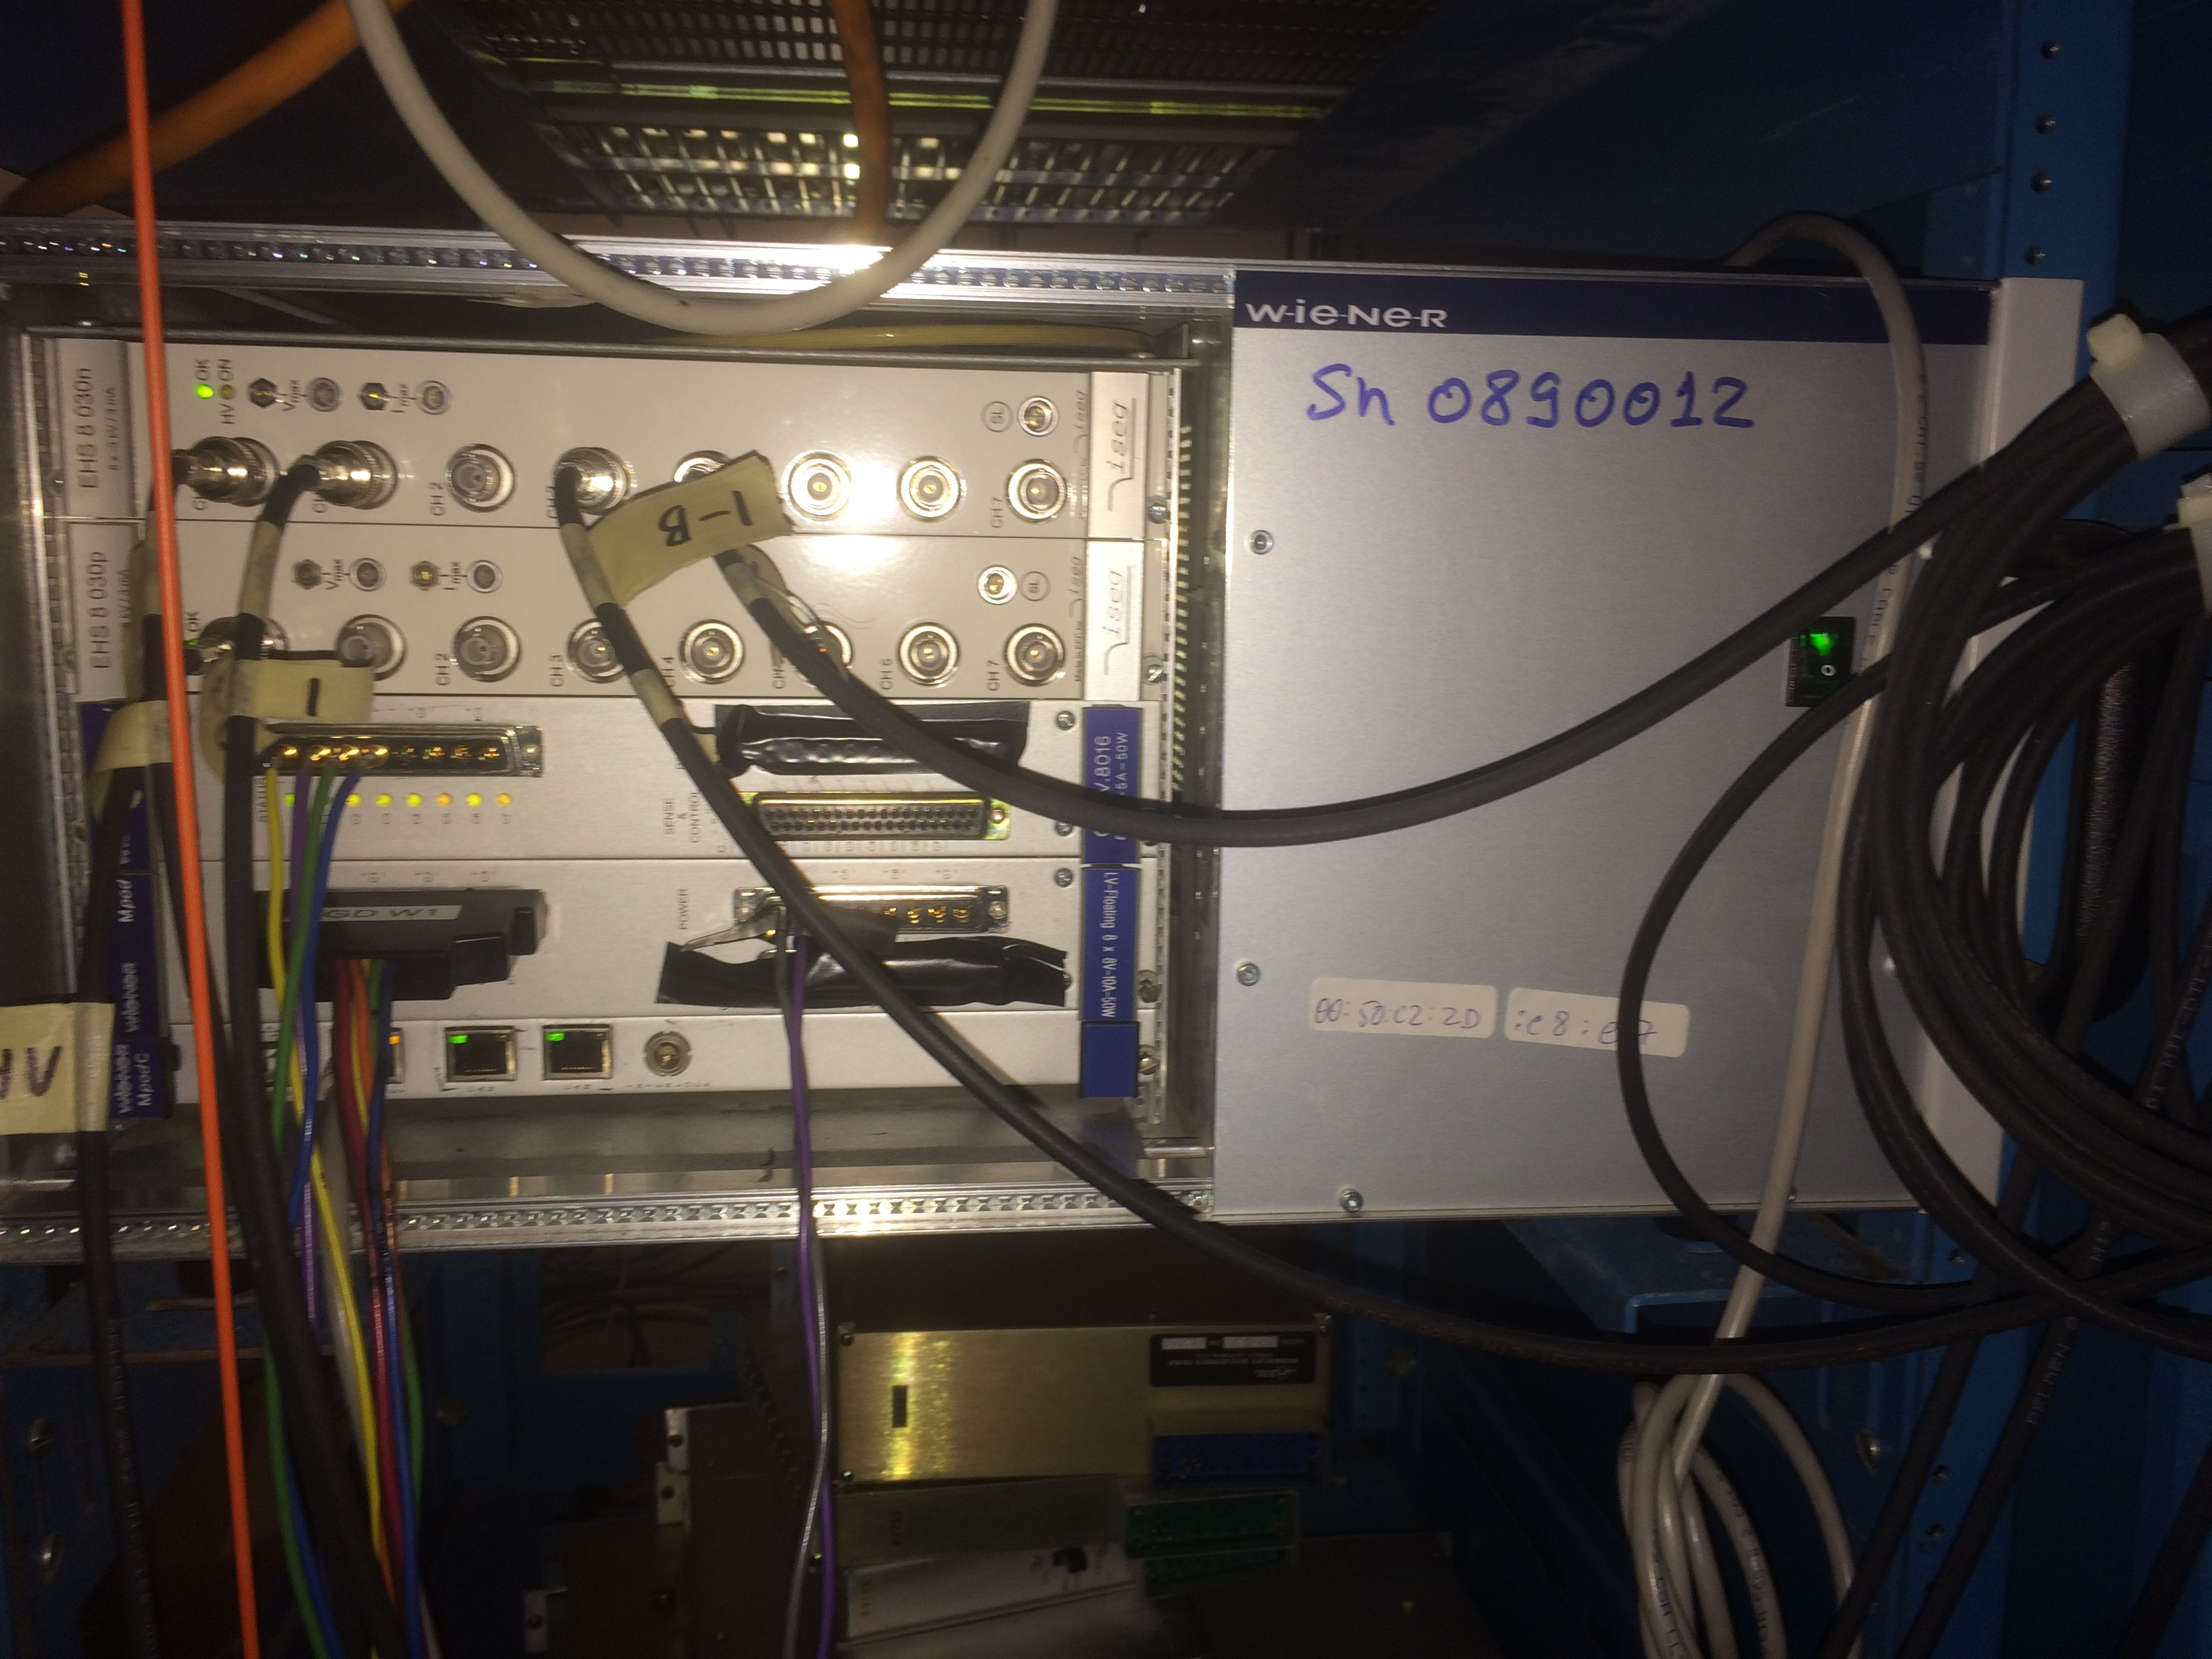
\includegraphics[width=\picwidth]{images/wiener}
	\caption{Wiener Crate\label{wiener}}
\end{figure}

\FloatBarrier

\clearpage

\subsubsection{Galil Motor Controller}

Provides control interface between Gantry Move program in \textbf{Movement Navigation Tab} and the motors controlling the motion of the gantry system itself. Powers the motors and tracks position by counting the motor's microsteps and the motor encoders quadrature pulses. Controlled by the PDU.\@ The Galil Motor Controller is located in the main equipment rack as shown in Figure~\ref{mainEquipmentRack} on the left.

\subsubsection{Hamamatsu Laser}

Provides 405nm laser beam to gantry optical box. Picosecond laser pulses are generated in a laser tube in a small box on the main equipment rack as shown in Figure~\ref{laser} and delivered to a single optical box via fiber optic cable.

\FloatBarrier

\begin{figure}[!htpb]\centering	
	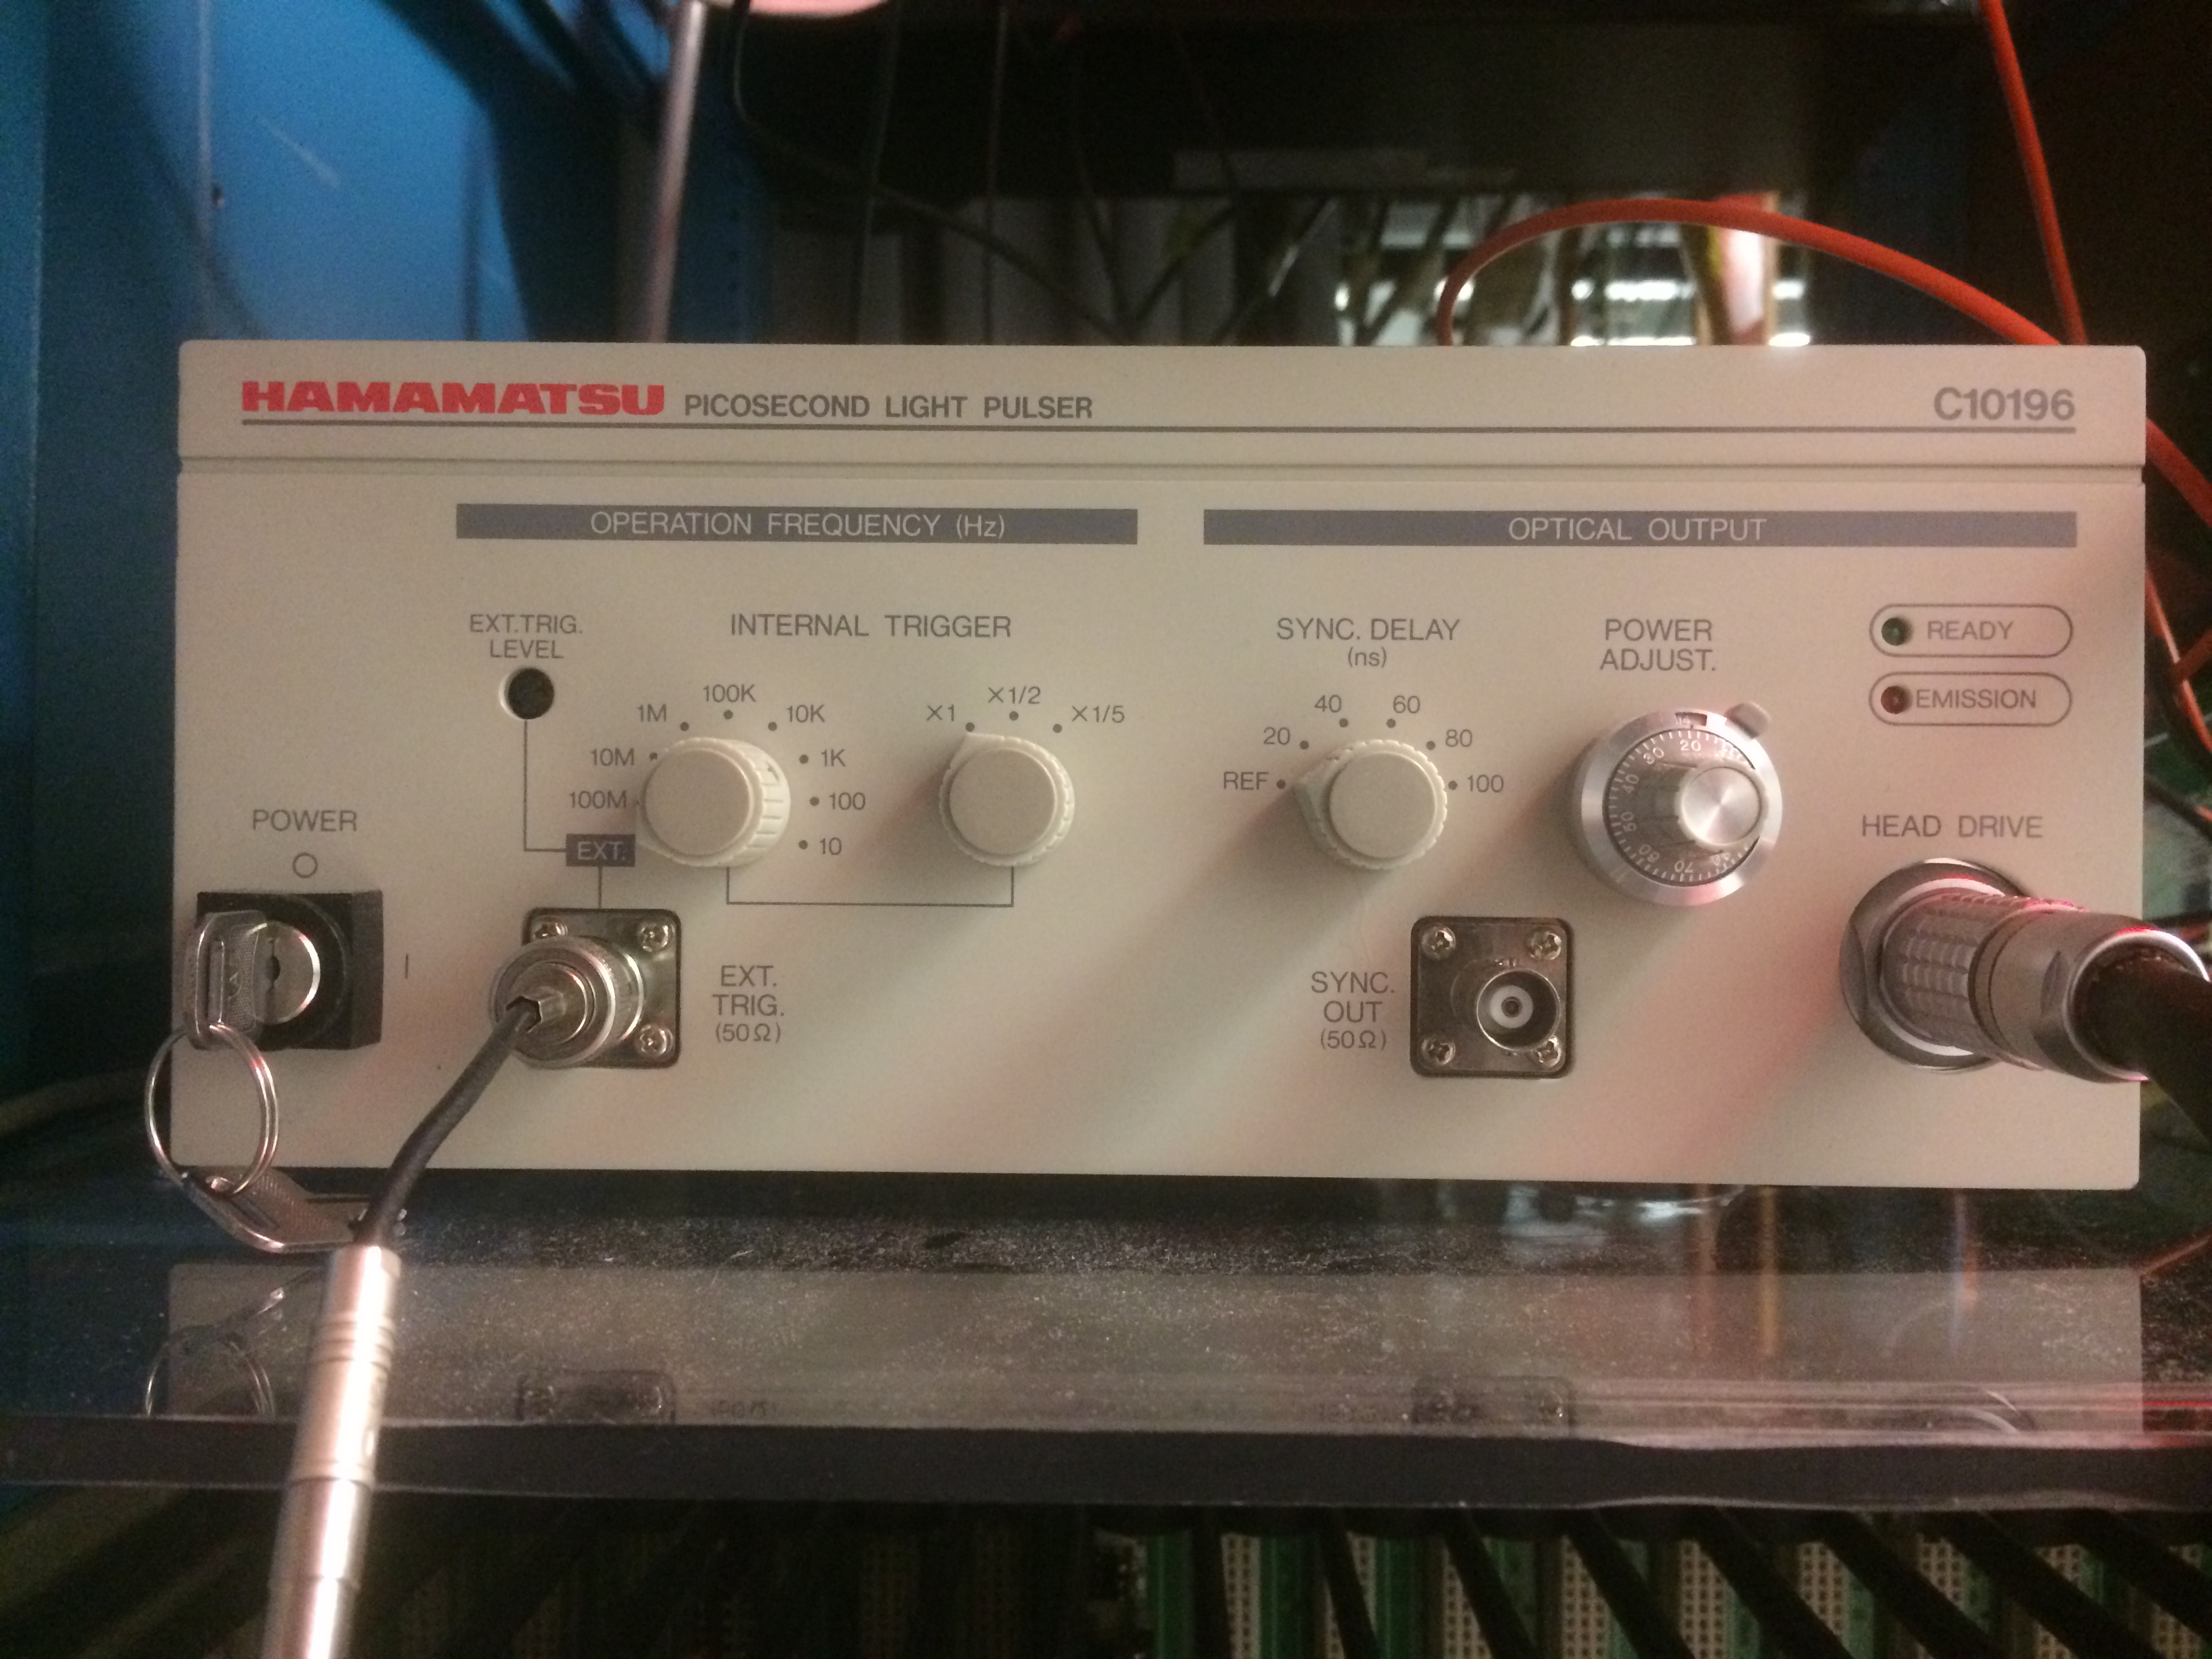
\includegraphics[width=\picwidth]{images/laser}
	\caption{Hamamatsu Laser\label{laser}}
\end{figure}

\FloatBarrier

\clearpage

\subsubsection{VME and NIM Crates (Data Acquisition and Triggering)}

The VME Crate provides power to the electronics which process and capture the PMT signal (waveform digitizer, pulse generator, etc). The VME Crate is located in the main equipment rack as shown in Figure~\ref{mainEquipmentRack} and Figure~\ref{vme}.

\FloatBarrier

\begin{figure}[!htpb]\centering	
	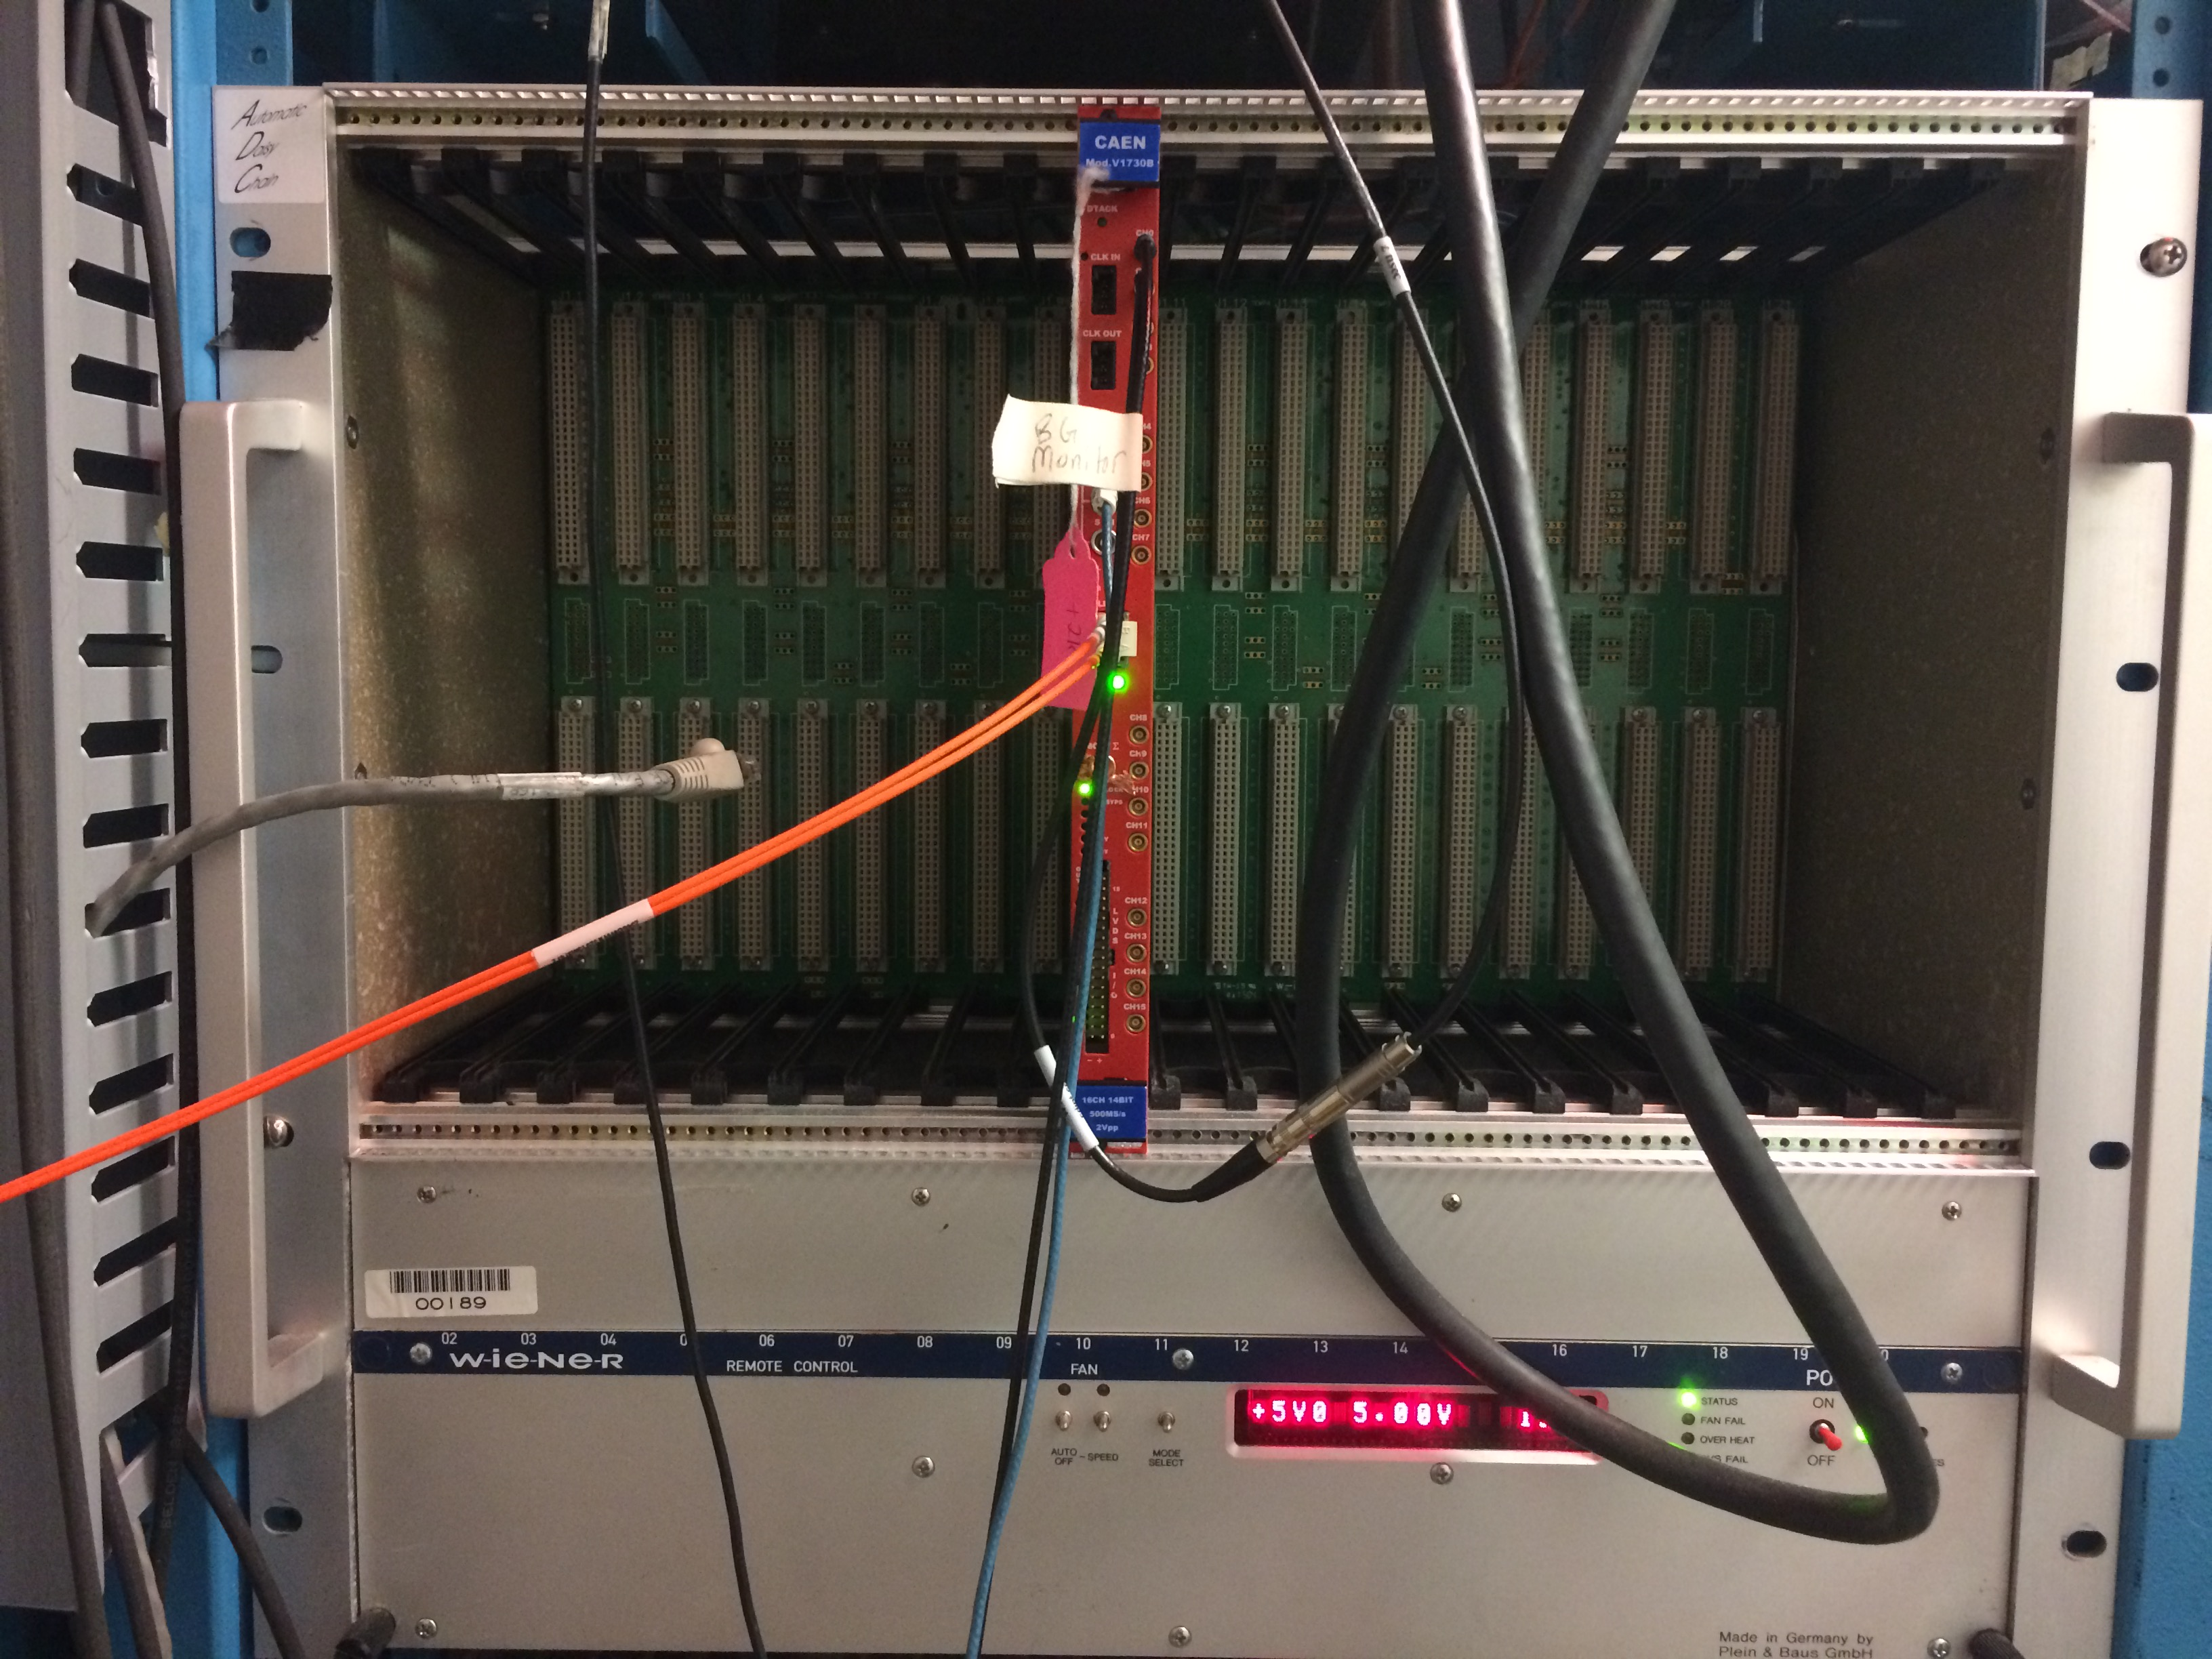
\includegraphics[width=\picwidth]{images/digiCrate}
	\caption{Waveform Digitizer\label{wvDigi}}
\end{figure}

\FloatBarrier

Important to note is the order of the various signal cables into the waveform digitizer.

\begin{enumerate}
	
	\item Primary PMT Signal (CH0)
	\item Reference Signal from Laser (CH1)
	\item Gantry 0 Receiver PMT Signal (CH2)
	\item Gantry 0 Monitor PMT Signal (CH3)
	\item Gantry 1 Receiver PMT Signal (CH4)
	\item Gantry 1 Monitor PMT Signal (CH5)
	
\end{enumerate}

These channels correspond to data acquisition channels in the recorded ROOT files when data is being collected. Also important to note is the optical fiber to the neut07 computer (orange). This is rather delicate and must be handled with care (read: do not kink or step on). As well, the signal cable from the pulse generator to the waveform digitizer must be connected.

\FloatBarrier

\begin{figure}[!htpb]\centering
	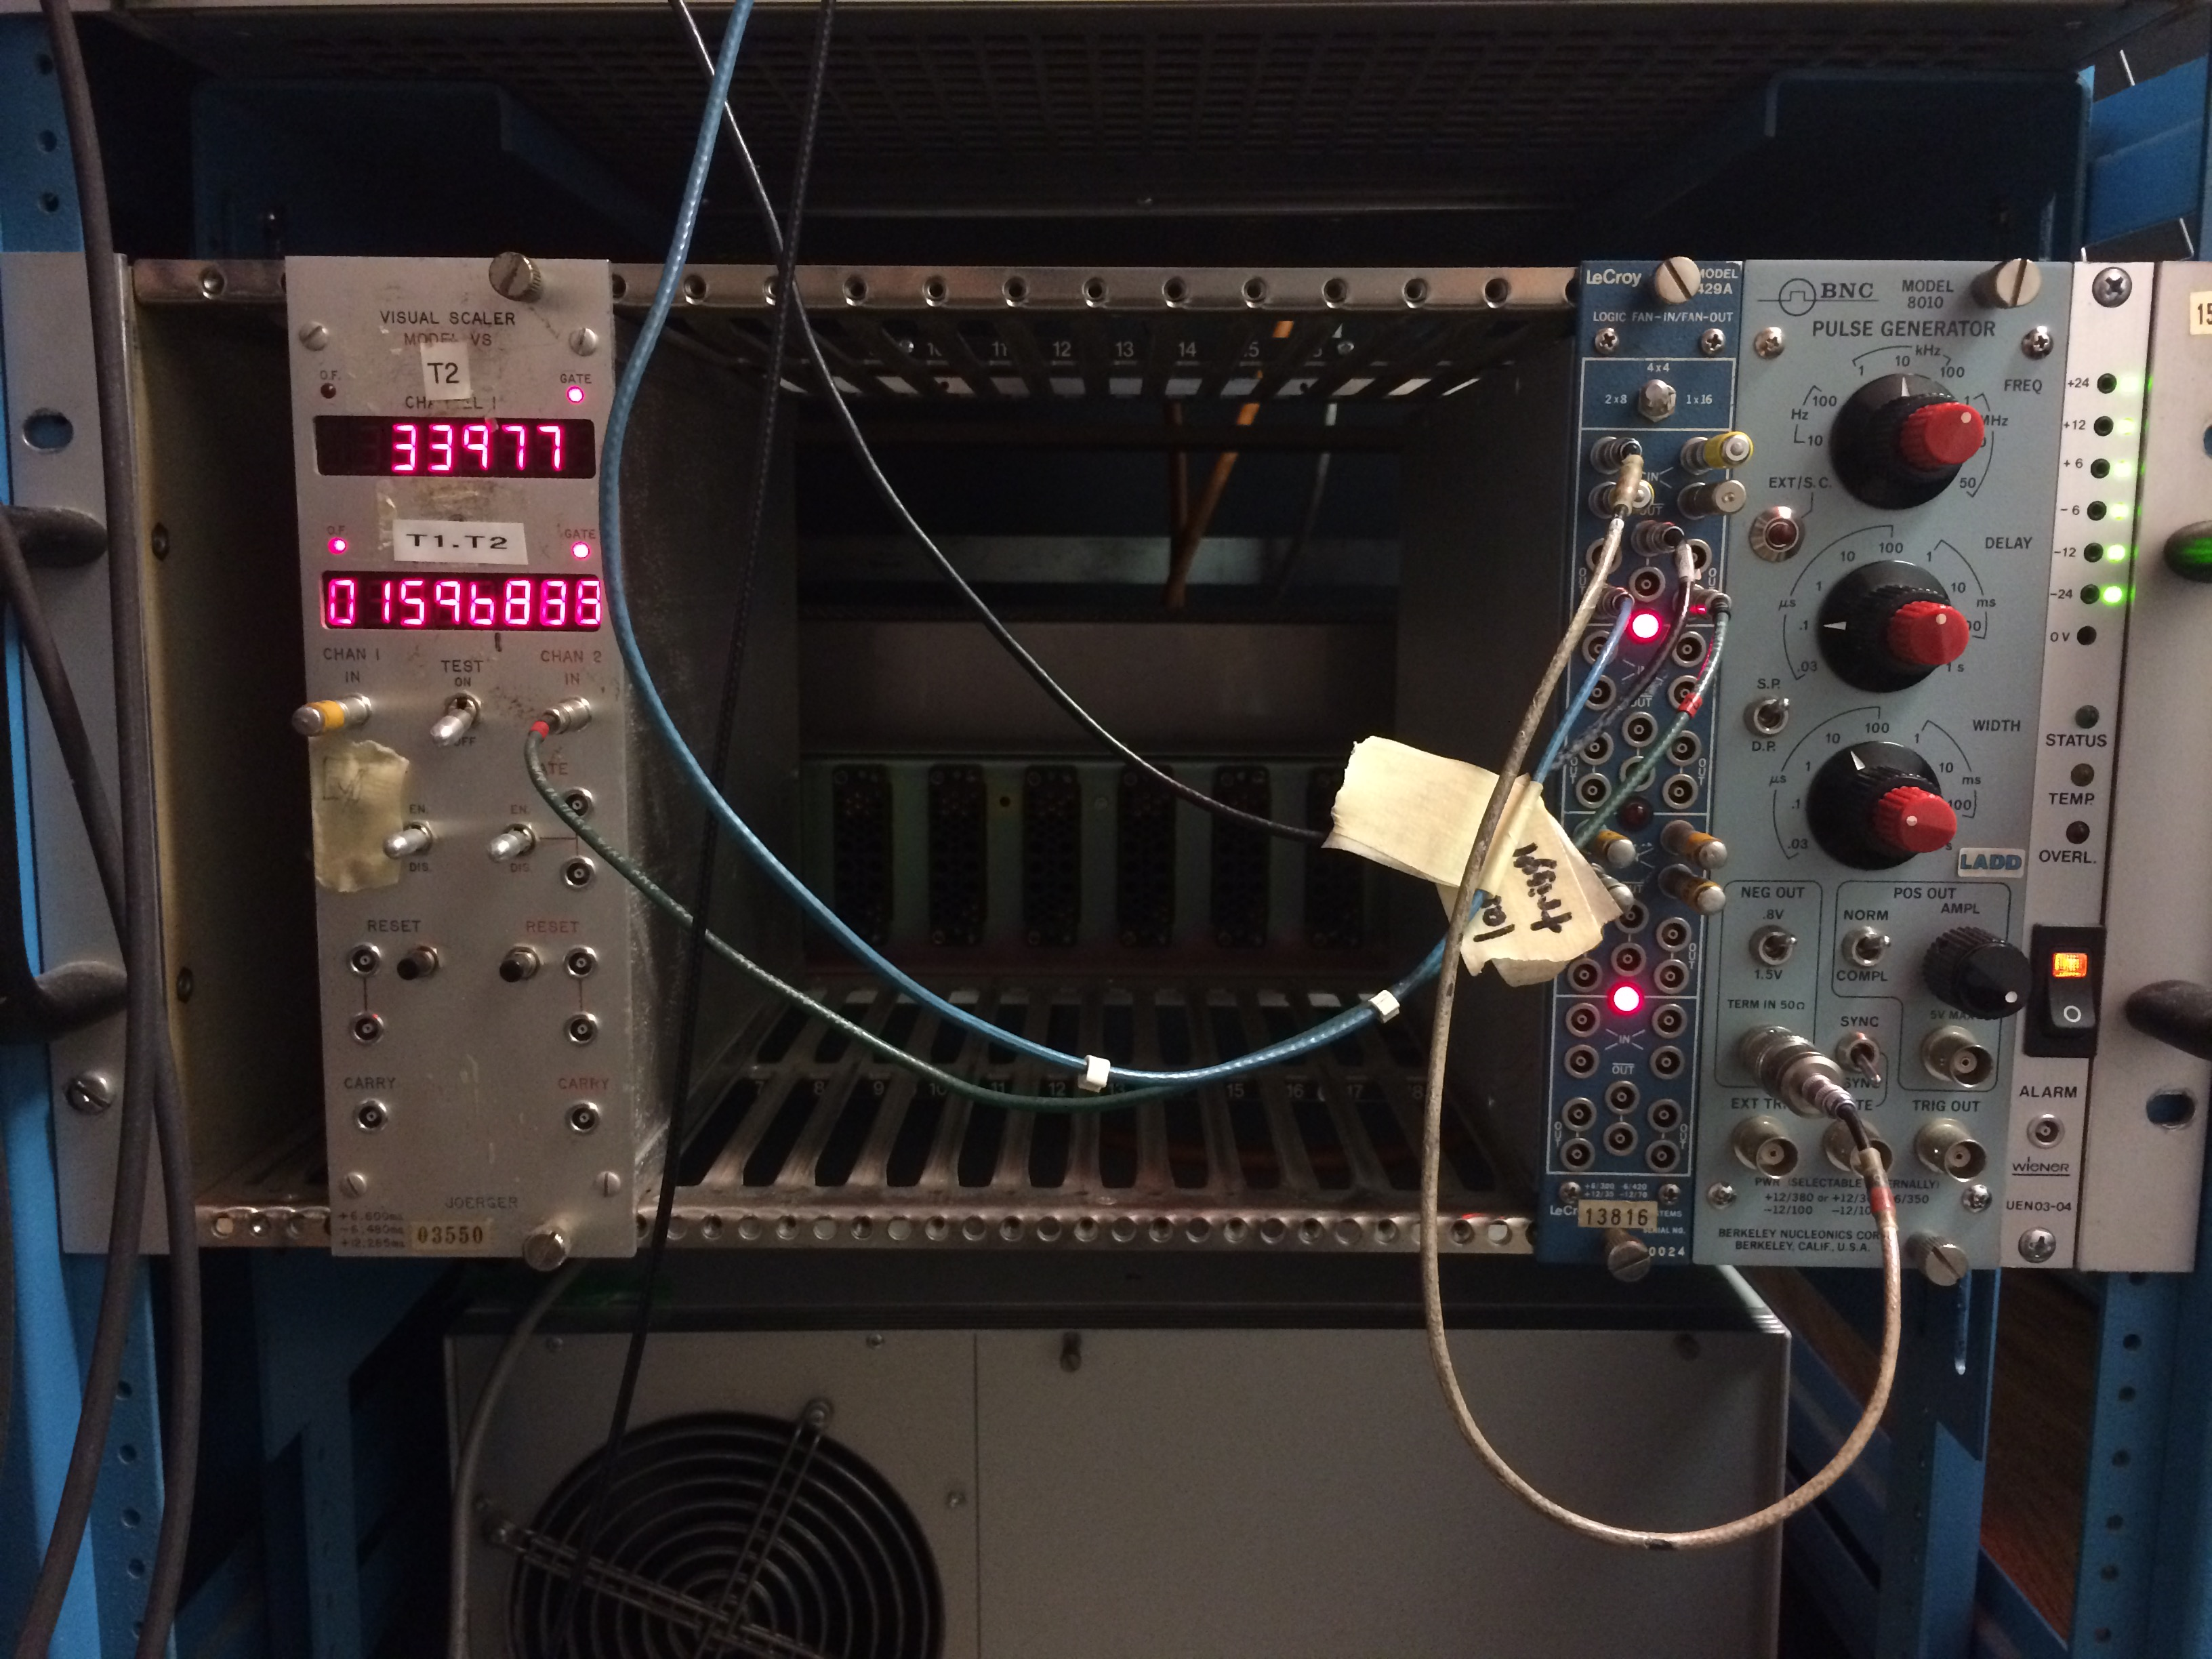
\includegraphics[width=\picwidth]{images/nimCrate}
	\caption{Trigger Pulse Rack\label{vme}}
\end{figure}

\FloatBarrier

The trigger pulse rack contains a counter (left) and a pulse generator (right), which sets the frequency of the laser pulses incident to the PMT.\@ This can be adjusted to achieve desired data acquisition speeds as long as the data can still be read out from the digitizer appropriately. The frequency dial is scaled by about a factor of 10 so the actual trigger frequency should be read from the \textbf{Events[/s]} value close to FEV17300OPTIC on the midptf status page during a run. Currently scans are performed at about 1600 Hz. Scans are performed at a default 3 seconds per point to provide a total of about 5000 waveforms per point.



\subsubsection{PMTs}

\paragraph{SK PMT}

The PMT located in the water tank under the acrylic cover is the Super Kamiokande PMT.\@ In the current configuration, the PMT that is in place is an R3600 model from Hamamatsu, with a 20 inch photocathode diameter.

%TODO: include picture

\paragraph{mPMT}

The multi-PMT (mPMT) is a prototype for the photosensors that will go into Hyper Kamiokande. Instead of a single large PMT, they're made up of many smaller PMTs which sacrifice some detecting area for a large increase in resolution. In addition, the acrylic cover and optical gel were included in the original design to help prevent implosion cascades.

%TODO: include picture
\clearpage
\subsubsection{Magnetic Field Control}

Magnetic fields can have a large effect on PMTs, especially larger ones such as the 20'' SK PMT\footnote{The magnetic field can affect the path of photoelectrons.}. As the PTF is close to the cyclotron, there is a very large magnetic field present. There are two types of compensation present: passive shielding from the G-Iron mesh surrounding the PMT tank, and active compensation from the six Helmholtz coils seen in Figure~\ref{fig:pmtAndCoils}. Detailed information is provided in Section~\ref{sec:magField}.

%An ambient magnetic field has been shown to have effect on various characteristics of PMT response, and as such the Helmholtz coil system in place is designed to control the ambient magnetic field within the PMT volume by means of active compensation. The design of the Helmholtz coil consists of 3 pairs of wire coils oriented along each axis in the gantry system space. Current through each coil is adjusted in order to produce a homogeneous field inside of a volume contained within the boundaries of the coils.

%In order to improve the effectiveness of the active compensation, passive compensation is implemented in the form of a sheet of G-Iron at the base of the PMT and a G-Iron cylinder concentric to the primary axis of the PMT. This limits the gradient of the field in the all directions in gantry space and enables a decoupling of the effects of field compensation in perpendicular directions. Additionally, if the cyclotron is ON, asymmetric coil currents in the Z-direction allow for the gradient to be controlled to an even finer degree, albeit with some added complexity.

\begin{figure}[!htpb]\centering	
	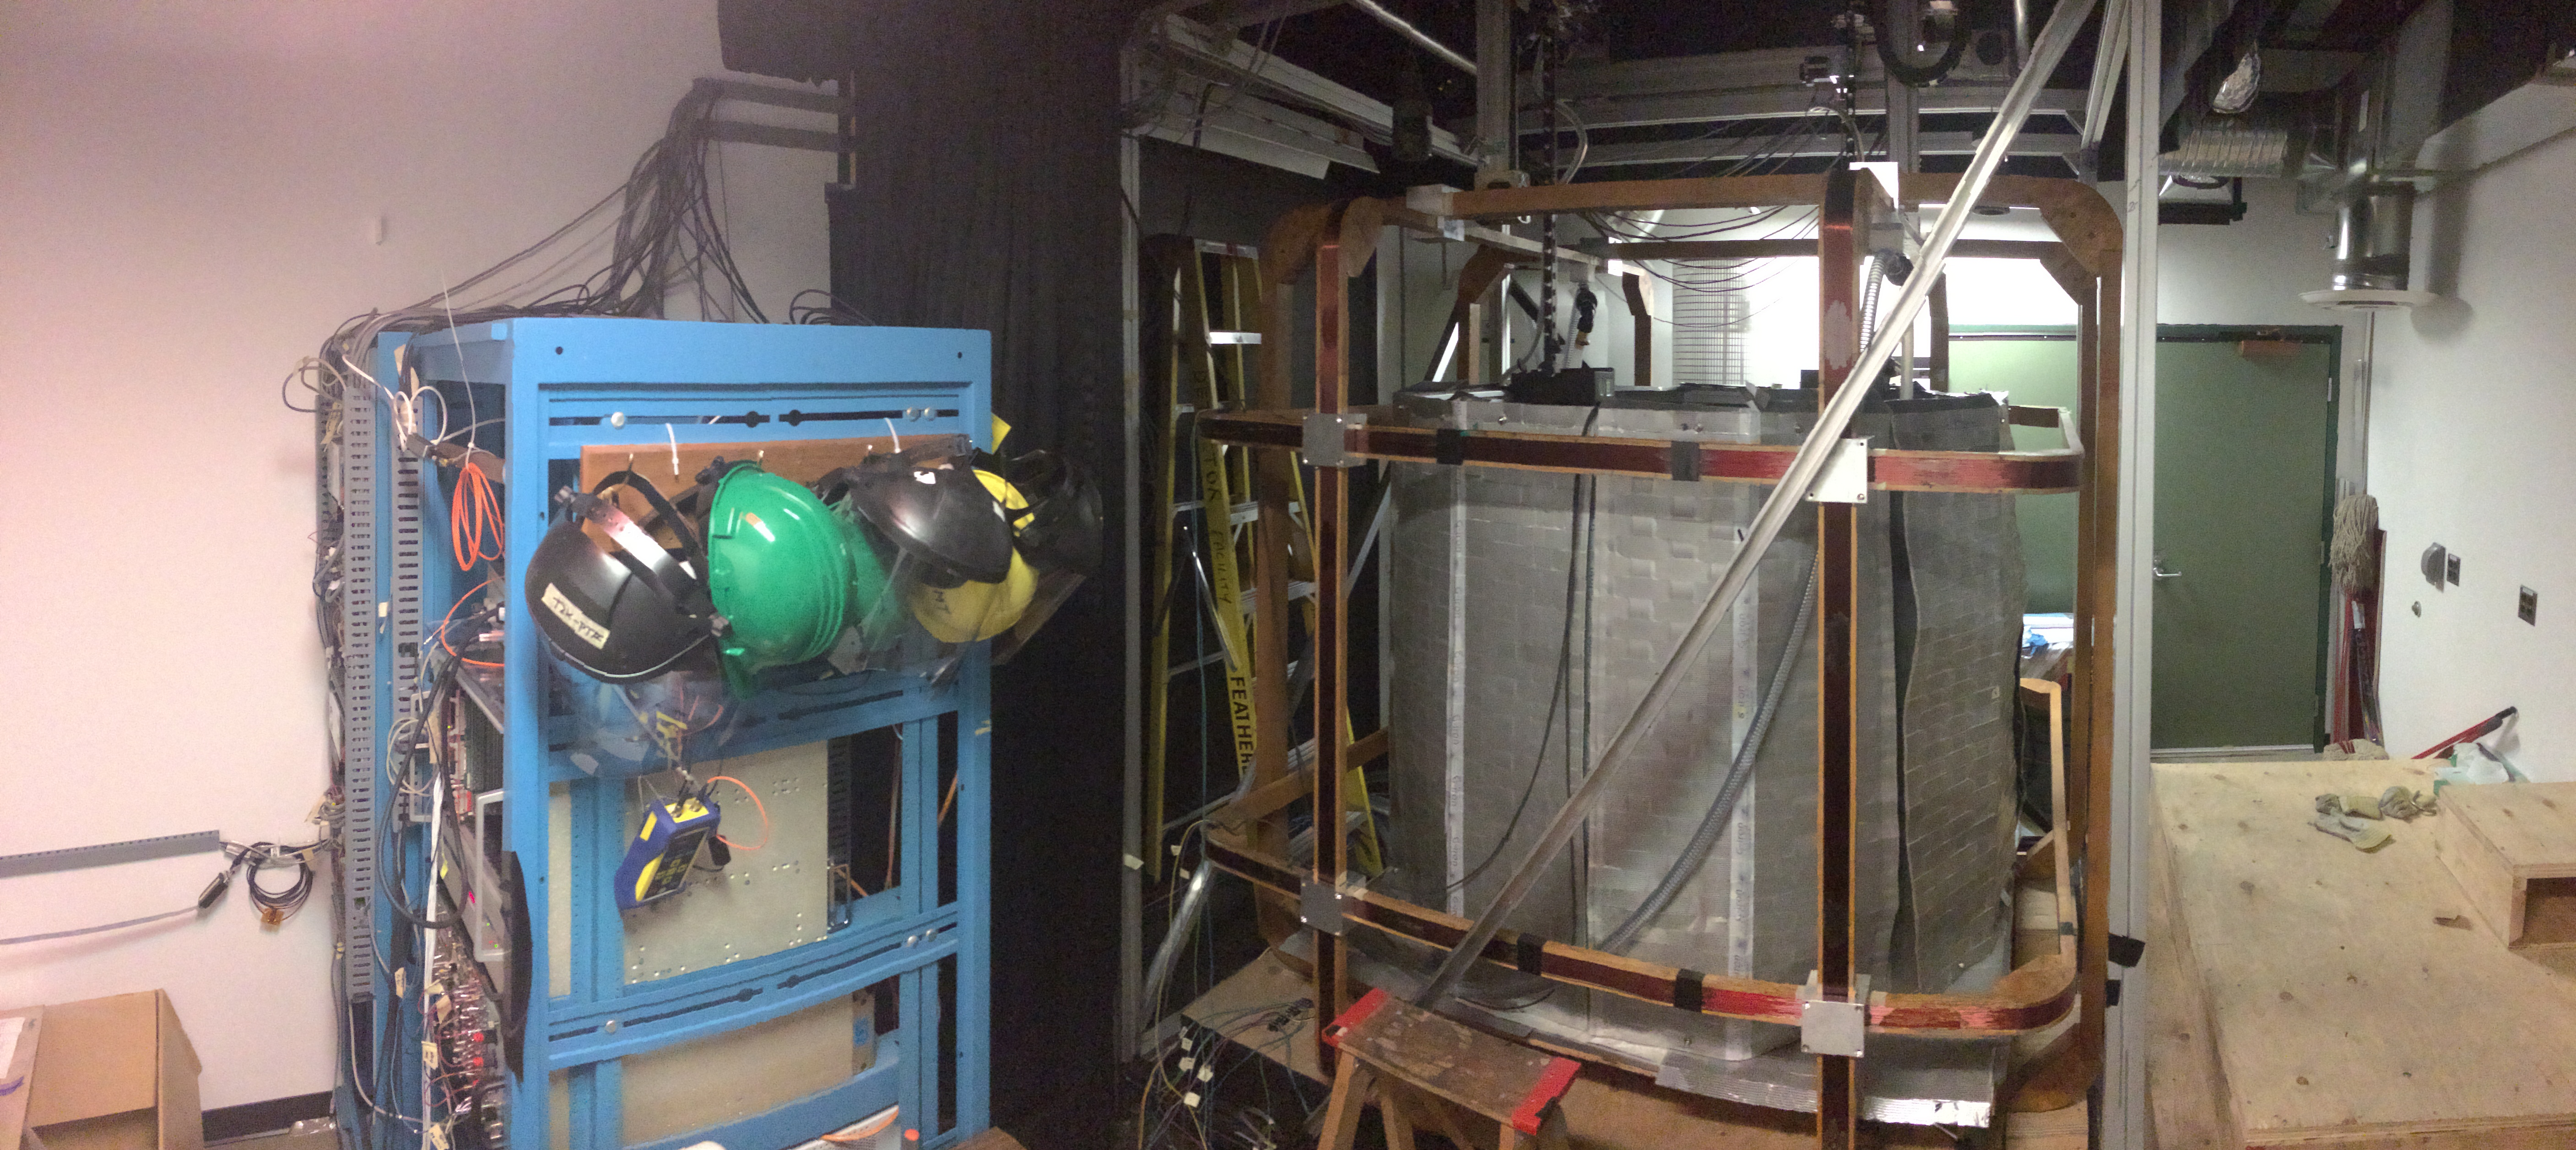
\includegraphics[width=\textwidth]{images/panoPTF}
	\caption{PMT and Helmholtz Coils\label{fig:pmtAndCoils}}
\end{figure}



\subsubsection{Phidgets}

``Phidgets'' are the name we use for the combination accelerometer/magnetometer USB sensors used in the PTF. They are used to calibrate both the magnetic field inside the coils and the tilt of the gantries. Each gantry has a phidget inside of it, numbered phidget 0 (for gantry 0) and phidget 1 (for gantry 1). There are additional phidgets around the PTF, which can be dynamically mapped to different numbers through the ODB.

%TODO: include picture of phidgets with and without covers

\begin{figure}[!htpb]\centering
	\includegraphics[width=0.3\textwidth]{images/Phidget_with_Casing.jpg}
	\includegraphics[width=0.3\textwidth]{images/Phidget_without_Casing.jpg}
	\caption{A spatial phidget accelerometer/magnetometer\label{fig:phidget}}
\end{figure}

\FloatBarrier

\clearpage


\subsection{PTF Setup}

Before any experiment can be performed, there are a number of hardware and software systems that must be powered and initialized for proper operation of the facility.

\subsubsection{Powering Up and Initialization}

Firstly, the computer in the PTF (\textbf{midptf01}) must be powered on. This computer runs the MIDAS data acquisition server and communicates with all of the equipment. From this computer (either directly in the PTF or over the network) it is possible to access the \textbf{HV} control for the coils and PMT, as well as all data obtained from measurements.

Once the computer is online, open a web browser and proceed to the main status page as described in Section~\ref{statusPage}. Once logged in, check the current status of the run as in Section~\ref{runStatus} and click on the \textbf{Programs} from the \textbf{Navigation Tabs} section (Figure~\ref{navTabs}).

If it is not turned on, the first program that must be started is the program \textbf{fepdu}. This allows frontend control of the \textbf{PDU} (Power Distribution Unit). Once this program is started, the next step is to navigate to the \textbf{Sentry Switched CDU} homepage. This interface can power on and off equipment. It is available at \href{http://midptf01.triumf.ca}{\texttt{http://midptf01.triumf.ca}}, while the MIDAS server is available at \href{https://midptf01.triumf.ca}{\texttt{https://midptf01.triumf.ca}}. Once the system is running, this page should only be used for remote laser power control and emergency shutdown. Use \texttt{admn} as the username and \texttt{pmtCalib123} as the password.

\begin{figure}[!htpb]\centering
	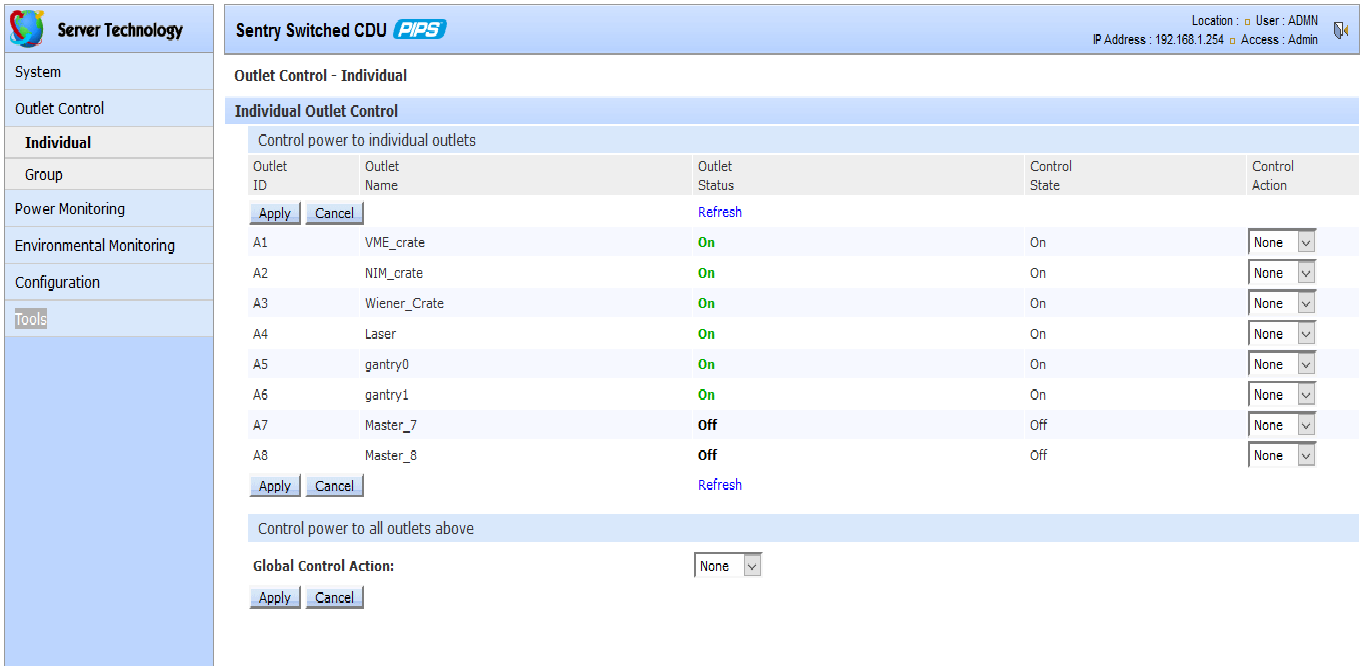
\includegraphics[width=\textwidth]{images/sentrySwitchedCDU.png}
	\caption{Sentry Switched CDU outlet control page\label{cdu}}
\end{figure}

On the CDU control page, navigate to \textbf{Outlet Control/Individual} and ensure the equipment is powered on as in Figure~\ref{cdu} by setting the Control Action for each outlet and clicking Apply.

\subsubsection{Frontend Initialization}

Once the various equipment pieces are powered on, the corresponding control software can be started. Software control of the equipment is accomplished via a series of \textbf{frontend} programs (see \href{https://midas.triumf.ca/MidasWiki/index.php/Frontend_Application}{the MIDAS documentation}), denoted by the prefix \textbf{fe} (eg. \textbf{feMove}, \textbf{feMotor}, \textbf{feScan}). If all of the electronics systems are powered on and initialized correctly, the following frontend programs must be turned on from the \textbf{Programs} tab in no particular order:

\begin{itemize}
	
	\item \textbf{Logger}: Writes MIDAS data
	\item \textbf{feV1730Optic}: Waveform Digitizer data recording
	\item \textbf{feptfwiener}: Controls HV and LV
	\item \textbf{fePhidget00}, \textbf{fePhidget01}, etc: Magnetic field and tilt monitoring (all phidgets, with 00 and 01 corresponding to the devices on Gantry0 and Gantry1)
	
\end{itemize}

Once those programs are turned on, the control programs for the motors can be turned on as well. Unlike the other programs, the order in which these programs are started is important. \textbf{feMove} must be started after both \textbf{feMotor00} and \textbf{feMotor01}.

\begin{itemize}
	
	\item \textbf{feMotor00}
	\item \textbf{feMotor01}
	\item \textbf{feMove}
	
\end{itemize}

If all goes well, the \textbf{Equipment} section of the main status page should look like the the image in Figure~\ref{equipment}, with the exception of Scan being OFF for now and feV1730Optic being ON.

\subsection{Preparing the PTF for Operation}

Once all software and hardware components are turned on and navigation of the system becomes familiar, the PTF can be prepared for operation with the PMT fully powered on.

\subsubsection{Checking the PMT}

The PMT should be inside the tank, contained within the controlled volume of the Helmholtz coils. It is a good idea to check the inside of the tank and the surface of the PMT, and take note of any markings on the surface for future reference.

\subsubsection{Closing the Curtains}

In order to maintain a light-proof environment in the PTF, specifically in the region which contains the PMT\footnote{As PMTs are sensitive to the level of single photons, the amount of light in the room needed by humans would destroy the electronics in the PMT.}, there are two sets of curtains which must be drawn closed.

Closing the curtains is accomplished by pulling the curtain fabric around the Helmholtz coils, in a counterclockwise direction when viewing the room from the top. Starting from the equipment rack, the curtains pull all the way around the main gantry frame to the water tank. On the wall beside the water tank, there are two strips of velcro, each of which provides an anchoring point for the leading side of each curtain set.

The room is light-sealed by firmly pressing the velcro on the curtains to the velcro on the walls, from the floor to the ceiling. A stepladder may be required to seal the curtains at the ceiling.

There is a BNC cable strung through the curtains that will move with it. Hanging from the wall is the terminator for the laser. It will not fire unless the BNC cable is connected to the terminating piece. This may be plugged in once the velcro is sealed. It is required to disconnect the BNC from the terminator when opening the curtain.

Once the curtains are pulled all the way around the frame, the interface between the curtains and the floor must be sealed. This is performed by covering the loose edge of the curtains with a series of aluminum milled blocks.

% todo: insert picture

\subsubsection{Laser and Attenuator Setup}

Once the curtains are closed, the laser system can be prepared and powered on. To do so, ensure that the fibre from the laser box (Figure~\ref{laser}) is connected to one of the FA58M fixed attenuators. It is required to route the laser through two such FA58M attenuators, and then through the VOAMMF manual variable attenuator. Then ensure that the desired optical fiber cable is connected to the other end of the VOAMMF.

Through a series of attenuators, reliable single photon emission can be attained. Presently the settings for SPE, or sometimes called low intensity, are two FA58M in series, each providing 27 dB of attenuation, then through the VOAMMF at maximum length which provides an additional 20 dB, thus totaling 74 dB. Occasionally the PMT response at higher intensities is desired. For a case of 100 PE, the attenuation should be set to 10 dB by adjusting the optical fiber cables such that only the VOAMMF is attached, rotated halfway. The laser power output is set to 520, which should not be changed without consulting others. The reason for this is to maintain a stable optical power from the laser. If other light intensities are desired, the attenuators should be changed out to provide the desired optical attenuation. Other fixed attenuators of various length and attenuation are located in the PTF.

More information is provided in \href{https://midptf01.triumf.ca/elog/PTF/484}{E-Log 484}.

Note that due to supply issues the fixed attenuators can only be connected via SMA heads whereas everything else in the setup uses FC/PC heads.

Only one optical box can receive laser beam at a time. As such, the optical box to use must be chosen, in most cases arbitrarily as they are functionally identical, though as of April 2018 only gantry1 may be used as there is an issue with the optical fiber going to gantry0.

Once the appropriate connections are made, the laser can be turned on. This is performed through the PDU page for the outlet power control, and also by a key switch on the laser box itself. Turn the key to \textbf{1} to turn the laser on.

Once the curtain is sealed and the laser set appropriately, it is critical that the main room light is turned \textbf{off} and a flashlight used to navigate in the PTF.\@ Now the PMT(s) can be powered up.

\clearpage

\subsection{Critical Equipment Power-Up}\label{PowerUP}

Go to the MIDAS control page. From the HV tab, power to the Wiener power supply channels can be controlled, including power to the primary PMT.

\textbf{Note: If the curtains are correctly closed and the room lights are off, it is safe to turn on the power to the Primary PMT and the receiver and monitor PMTs in each optical box. If the curtains are open, only magnetic field studies and trial scans with the PMTs and Laser off can be performed.}

\FloatBarrier

\begin{figure}[!htpb]\centering	
	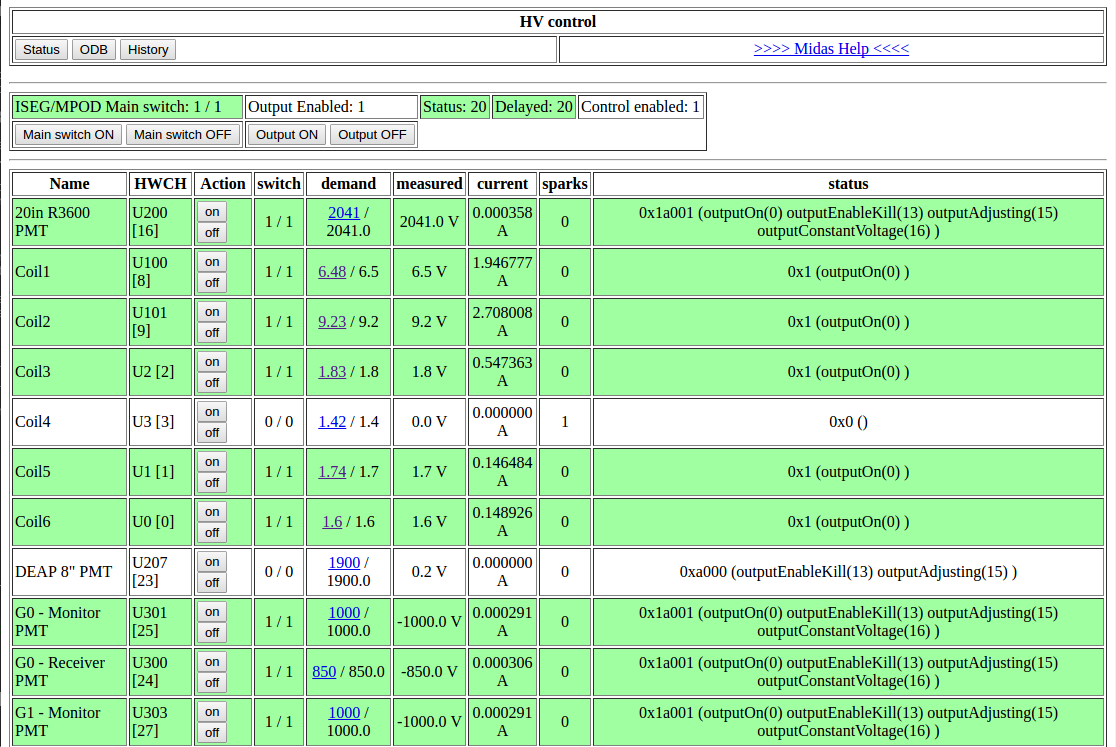
\includegraphics[width=\textwidth]{images/HVPage}
	\caption{HV Control Page\label{HVPage}}
\end{figure}

\FloatBarrier

The \textbf{ISEG/MPOD Main Switch} field, controlled by the buttons denoted ``main switch ON'' and ``main switch OFF'' indicates the status of the Wiener power supply. The \textbf{Output Enabled} field controlled by the buttons denoted ``Output ON'' and ``Output OFF'' indicates whether the different channels of the Wiener power supply are enabled for output. Please ensure that both the \textbf{ISEG/MPOD Main Switch} field and \textbf{Output Enabled} field are enabled by pressing the corresponding ON buttons as described above.

Once the power is enabled on the output channels, power can now be enabled for each channel of the power supply. A detailed listing of each channel is as follows:

\begin{description}
	
	\item[\textbf{20in R3600 PMT}] Controls Voltage of Primary PMT \\
	Channel: U200 \\
	Normal Voltage: 2041 V
	
	\item[\textbf{G0 --- Monitor PMT}] Controls Voltage of G0 Monitor PMT \\
	Channel: U301 \\
	Normal Voltage: 1000 V (Measured is negative)
	
	\item[\textbf{G0 --- Receiver PMT}] Controls Voltage of G0 Receiver PMT \\
	Channel: U300 \\
	Normal Voltage: 850 V (Measured is negative)
	
	\item[\textbf{G1 --- Monitor PMT}] Controls Voltage of G1 Monitor PMT \\
	Channel: U303 \\
	Normal Voltage: 1000 V (Measured is negative)
	
	\item[\textbf{G1 --- Receiver PMT}] Controls Voltage of G1 Receiver PMT \\
	Channel: U304 \\
	Normal Voltage: 850 V (Measured is negative)
		
	\item[\textbf{Coil1}] Controls Voltage of Coil 1 \\
	Channel: U100 \\
	Normal Voltage: Variable
	
	\item[\textbf{Coil2}] Controls Voltage of Coil 2 \\
	Channel: U101 \\
	Normal Voltage: Variable
	
	\item[\textbf{Coil3}] Controls Voltage of Coil 3 \\
	Channel: U2 \\
	Normal Voltage: Variable
	
	\item[\textbf{Coil4}] Controls Voltage of Coil 4 \\
	Channel: U4 \\
	Normal Voltage: Variable
	
	\item[\textbf{Coil5}] Controls Voltage of Coil 5 \\
	Channel: U1 \\
	Normal Voltage: Variable
	
	\item[\textbf{Coil6}] Controls Voltage of Coil 6 \\
	Channel: U0 \\
	Normal Voltage: Variable
	
\end{description}

\subsubsection{Powering the PMTs}

The power to the Primary PMT, and Monitor and Receiver PMTs can be turned ON if the curtain is closed as mentioned above. There is a ramp-up sequence, which should take approximately 60 seconds. The channels should be monitored for sparks (via software alert) during this period. Do not rapidly turn on and off the PMTs.

\subsubsection{Powering the Helmholtz Coils}

The power to the Helmholtz coil array can be turned ON.\@ It is important to set these correctly, as changing the voltage and current outputs on the coil channels will directly affect the magnetic field seen by the PMT, and will change the response of the PMT.\@ Correct setting of the coil currents is described in detail in a later section. Unlike the PMTs, the operational voltages of the coils are low but the currents are quite high (on the order of a few amps), so care should be taken if maintenance of the coils is required.

\subsection{Gantry Motion}

Movement of each gantry is controlled from the webpage accessible via the \textbf{Movement} tab of the navigation tabs in Figure~\ref{navTabs}.

\textbf{*Note: There is a collision avoidance path finding system in place, so movement of gantry 0 and gantry 1 can be performed with confidence that the gantries will not collide with each other, the tank or the PMT itself. The scripts controlling this are explained in a later section. It is good practice to check the collision avoidance if the tank has been moved. The user is notified if there is no valid path between the current position and the destination by a MIDAS message on the same page (not shown).}

\FloatBarrier

\begin{figure}[!htpb]\centering	
	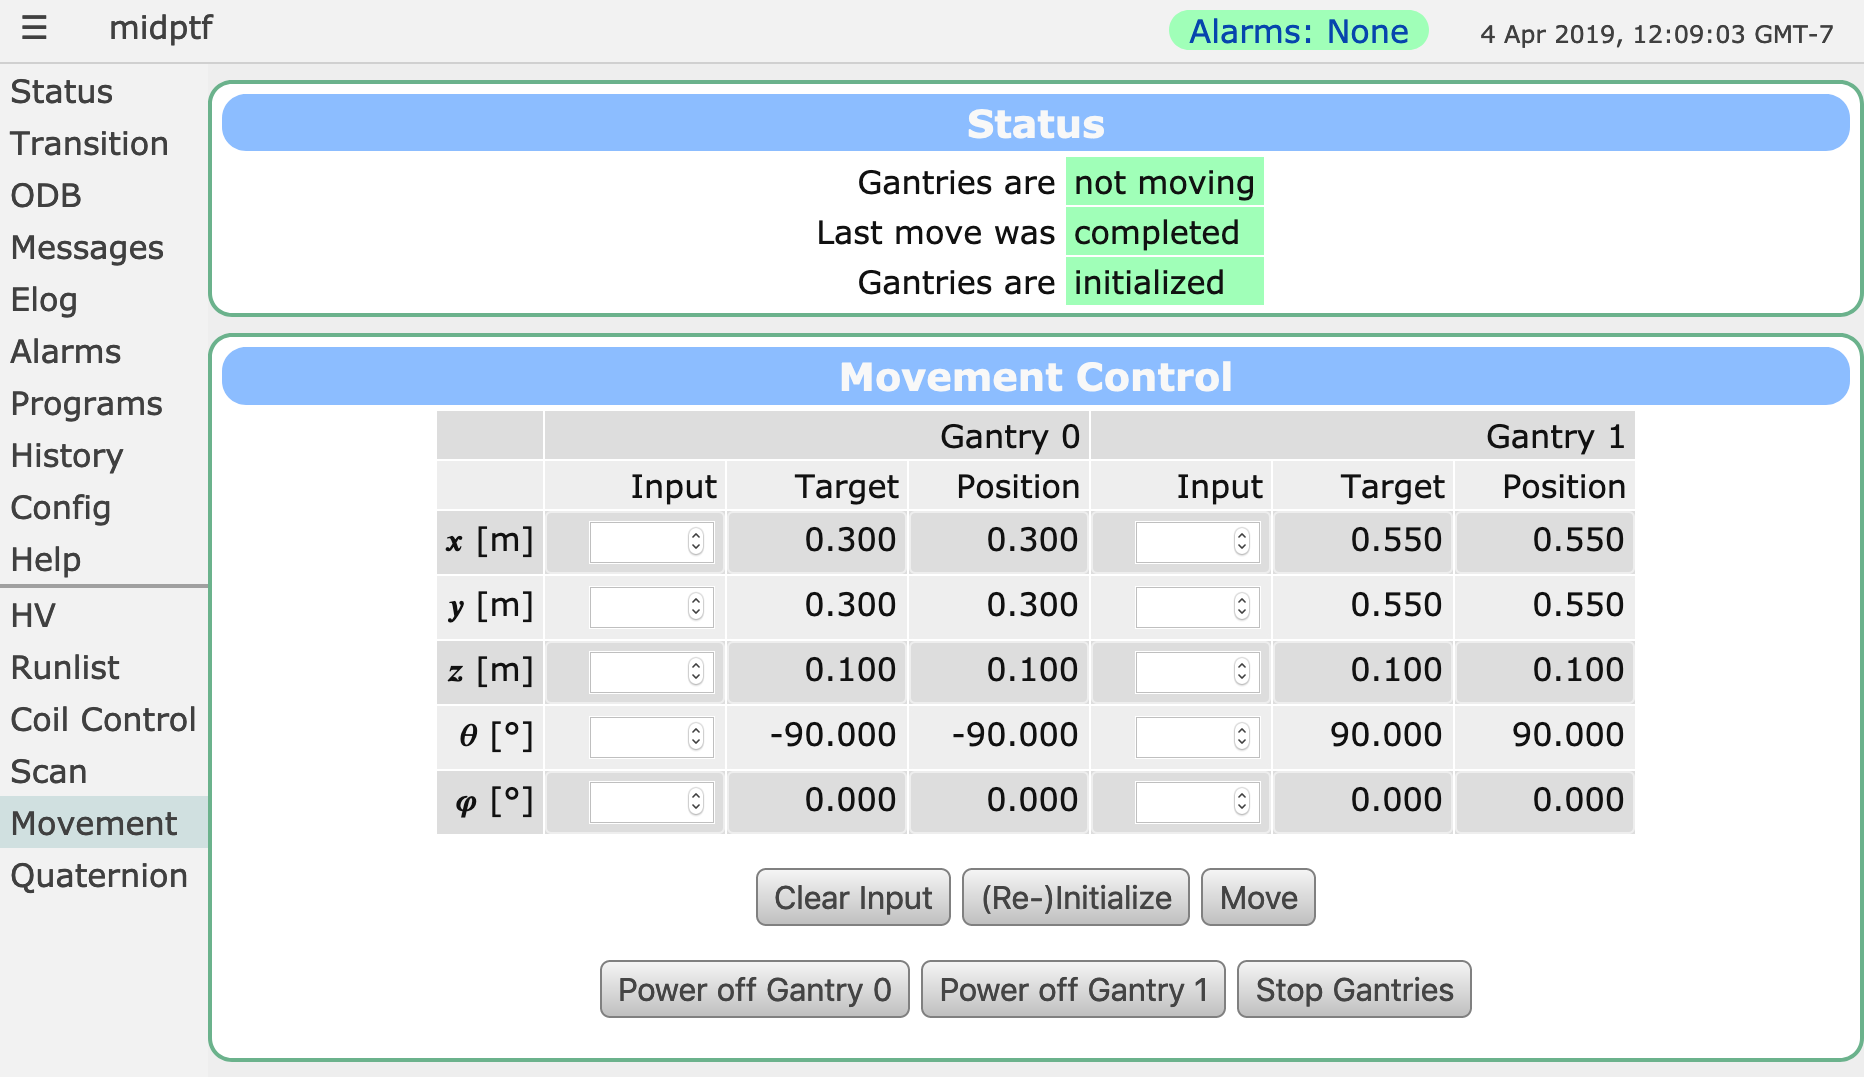
\includegraphics[width=\textwidth]{images/movement.png}
	\caption{Gantry Move Interface\label{gMove}}
\end{figure}

\FloatBarrier

The page in Figure!\ref{gMove} is divided into two main sections, \textbf{Status} and \textbf{Movement Control}.

\subsubsection{Gantry Status}
The Gantry Status simply displays whether the gantries are moving or not, whether the previous (or current) move has been completed, and whether or not the gantries have been initialized.

\subsubsection{Gantry Control}\label{GantryMove}

The Gantry Control section allows for motion and positional control of each gantry. For each gantry, there are three columns: input, target and position. The \emph{input} column is used for setting the positions that you would like the gantries to move to. The \emph{target} position is the position to which the gantries will move or are moving. This is set to the value of \emph{input} when you click ``move''. Finally, the \emph{position} field displays the currently measured position of the gantries. The buttons in this section are described as follows:

\begin{enumerate}
	\item[\textbf{Clear Input}] Clears any positions entered.
	
	\item[\textbf{(Re-)Initialize}] This moves the gantries (in a path that should never cause collisions) until they reach their limit switches in each direction. This serves as a point of reference for determining the position of the gantries, as each can only measure relative position. This will need to be done every time that the gantries power up or if there is doubt to the accuracy of their positioning.
	
	\item[\textbf{Move}] Execute the move entered in the control.
	
	\item[\textbf{Power off Gantry 0}] Turns off the stepper motors controlling gantry 0 motion. These motors contribute significant electrical noise, and so must be turned off manually when performing a single point measurement as in Section~\ref{singleData}. During a scan this function is implemented automatically.
	
	\item[\textbf{Power off Gantry 1}] Same function as the previous but for gantry 1.

	\item[\textbf{Stop Gantries}] Immediately halts motion of gantries.

\end{enumerate}

\clearpage

\section{Performing Measurements}

\subsection{Single Data Point Measurement}\label{singleData}

\subsubsection{Collecting Data}

%todo: update this section

Often, it is useful to perform a measurement at a single point on the PMT surface, either for system debugging, manual data collection or positional testing of the gantry. Performing a single measurement entails moving the gantry to a specified position as in Section~\ref{GantryMove} and collecting data from the PMT for that point.

There are two types of single point scans, the first of which does not have the \textbf{feScan} program running. To begin taking data at a single point, ensure that the laser beam is powered and connected to the gantry which will be moved, and that the curtains are closed and all equipment is properly powered as in Section~\ref{PowerUP}. Choose a point at which to position the gantry, and move it there as in Section~\ref{GantryMove}. At this point, the motors for the gantry must be turned off, as they will cause electrical noise in the collected data (this can be done in the GantryMove page).

Once the motors are turned off, and the attenuator line set to the standard value of 74 dB, the run can be started. This is done by pressing \textbf{Start} in the Run Status Section (\ref{runStatus}), and filling in the subsequent run log data (make this as clear as possible). If you want to keep the data collected in a ROOT file for future use, ensure that the option ``Write data to file'' is selected, otherwise data will not be collected.

The second type of single point scan has \textbf{feScan} on with Scan Type set to \textbf{Manual}. This type of scan functions similarly to a regular scan in that its measurements are done in intervals over a distinct number of scan points, and can be used to produce a regular analysis-compatible ROOT file that may be used to monitor the PMT response of a single point over long periods of time. The coordinates and number of points in this scan presently must be specified in the script \texttt{ScanSequence.cxx}.

\subsubsection{Viewing Data}

Once the run is started, there is a tool that can be accessed to view collected data in real-time. This tool is located on \textbf{midptf01} under the user \textbf{midptf} with the command `ptfDisplay' (or with the file path \textbf{/packages/rootana/examples/anaDisplay.exe}). Running this will provide an interactive instance of the ROOT analysis package, providing a list of histograms with data currently being collected.
There are two tabs available in the windowed program, V792 and V1730 Waveforms. Currently, only the V1730 Waveforms tab contains relevant data. This tab shows 1 of 100 events occurring on the waveform digitizer as it is recorded. Histograms within the tab are labelled 0--31 and correspond to the 32 output channels of the waveform digitizer in Figure~\ref{wvDigi}. Waveform 0 is the PMT signal and Waveform 1 is the reference pulse from the synchronized laser pulse generator. As well, the PMT output can be attached to an oscilloscope and the actual waveforms can be monitored. This is helpful when troubleshooting or adjusting attenuation levels to find single photon events.

Additionally, if the option is selected to write data to a ROOT file, additional analysis can be performed externally using custom ROOT scripts (available for cloning from \href{https://bitbucket.org/ttriumfdaq/ptf-analysis}{here} or the local clone on \textbf{midptf@midptf01} at \texttt{/online/src/analysis\_scripts/}).

\subsection{Magnetic Field Control and Degaussing}

The state of the magnetic field in the PMT volume has been observed to significantly influence PMT response, and as such it is crucial that magnetic field control be implemented at all stages of the data collection and measurement pipeline. See Section~\ref{sec:magField} for more information on how the field was calibrated.

There are two types of magnetic field control in place, a \textbf{G-Iron} shield referred to as passive shielding, and an array of \textbf{Helmholtz Coils} also referred to as active compensation. These shielding methods allow a reduction in both the gradient and the magnitude of the magnetic field in all three axes of the PMT volume by almost 2 orders of magnitude. The ambient field from the cyclotron in the PTF without compensation is on average 1800mG, with the primary component being in the Z-Direction. With compensation it is possible to obtain maximal gradient and magnitude of the field inside the PMT volume on the order of 15mG, smaller than the average field in the Super-K experiment.

\subsubsection{Degaussing}

Due to the high magnetic permeability of the material used for passive shielding, there is a non-negligible contribution to the measured field from the magnetic dipole alignment of the material which presents itself as hysteresis\footnote{Path dependence. Setting the coils to the same value will produce different fields depending on the path taken to those voltages.}. To reduce this hysteresis, a degaussing procedure has been designed to remove any non-random dipole alignment and thus provide a neutral state from which to adjust the magnetic field via the active compensation.

To degauss, we follow a particular path to the final voltages that produces a consistent field. The path chosen starts as far away from the desired voltages as possible, then gets exponentially closer while alternating being above and below the target voltage.

\subsubsection{Setting Coil Currents}\label{setCoils}

The adjustment of coil currents is achieved by accessing the Coil Control tab from the navigation tabs in Figure~\ref{navTabs}. The page is similar to that which is used to manipulate the gantry, and provides feedback on the current state of the magnetic field. The page is shown in Figure~\ref{fig:helmCoil}. On the left is a readout from all of the phidgets (whether they're actually working or not), and on the right is a control for the coils. The two buttons, \emph{switches on} and \emph{switches off} turn the power for the coils on and off. To individually set the voltage of each coil, click on the values in the ``target voltage'' column. Coils 3--6 are limited to 8V each, and Coils 1 and 2 are limited to 15V.

To degauss, use the ``Degauss'' section. Set each of the final voltages and the number of steps (eight is recommended). Then, use ``Start Degauss'' to run it. A progress bar will appear showing how much of the degauss is complete (see Figure~\ref{fig:helmCoilDegauss}).

\FloatBarrier

\begin{figure}[!htpb]\centering	
	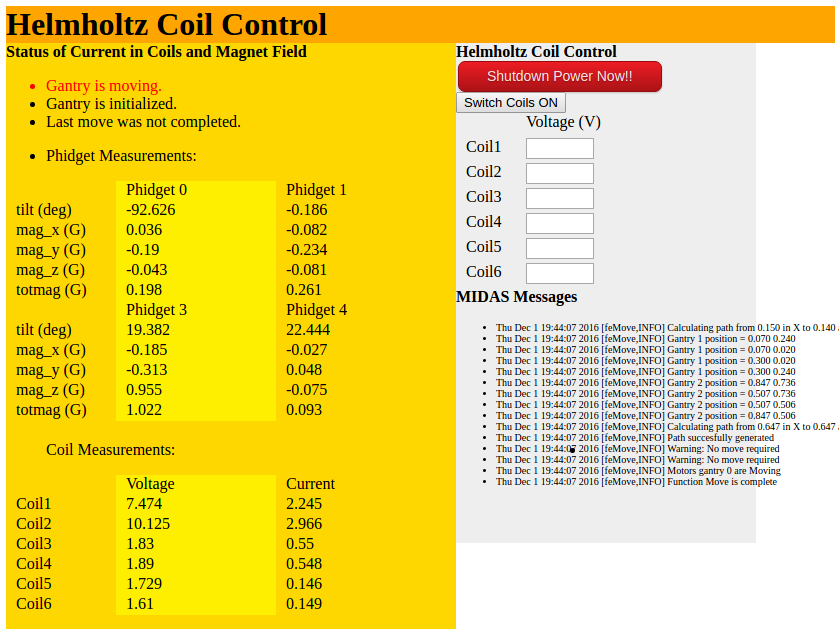
\includegraphics[width=\textwidth]{images/helmCoil}
	\caption{Helmholtz Coil Control Page\label{fig:helmCoil}}
\end{figure}

\begin{figure}[!htpb]\centering
	
\includegraphics[width=\textwidth]{images/helmCoilDegaussing}
	\caption{Interface during a degauss\label{fig:helmCoilDegauss}}
\end{figure}

\FloatBarrier


\subsubsection{Sources of Variation in the Field}

There are many components to the field observed in the PTF.\@ The largest and most obvious (other than the Earth) is the cyclotron. Separate calibrations must be used for when the main magnet is on and for when it is off. You can check the status of the field and current work on the \href{https://cycops.triumf.ca/}{Cyclotron Operations page}.

\subsubsection{Values to Use}

As of the time of writing, there are no fully compensated values to use. A new study when the cyclotron is on is pending.

\FloatBarrier

\begin{table}[htb!]\centering
	\begin{tabular}{rrrrrrr}
		\textbf{Cyc. Status} & \textbf{Coil 1} [V] & \textbf{2} [V] & \textbf{3} [V] & \textbf{4} [V] & \textbf{5} [V] & \textbf{6} [V] \\\toprule
		Off & 1.922 & 2.590 & 1.542 & 2.460 & 2.316 & 1.005 \\
		On & \\\bottomrule
	\end{tabular}
\end{table}

\FloatBarrier


\subsection{Measurements with PMT and Laser OFF}

It is sometimes useful to be able to take measurements without the PMTs and laser ON, either to measure an environmental condition or to test a new feature implemented in the PTF.\@ To do so, simply ensure that the PMTs and laser are powered OFF, open the curtains, and perform a scan or measurement as detailed in Section~\ref{AreaScan} or Section~\ref{singleData}.


\subsection{Area and Volume Scans}\label{AreaScan}

There are multiple types of scans than can be done in the PTF.\@ Each has its own set of parameters which can be set in the interface. A picture of this can be seen in Figure~\ref{fig:scanParams}.

\FloatBarrier
\begin{figure}\centering
	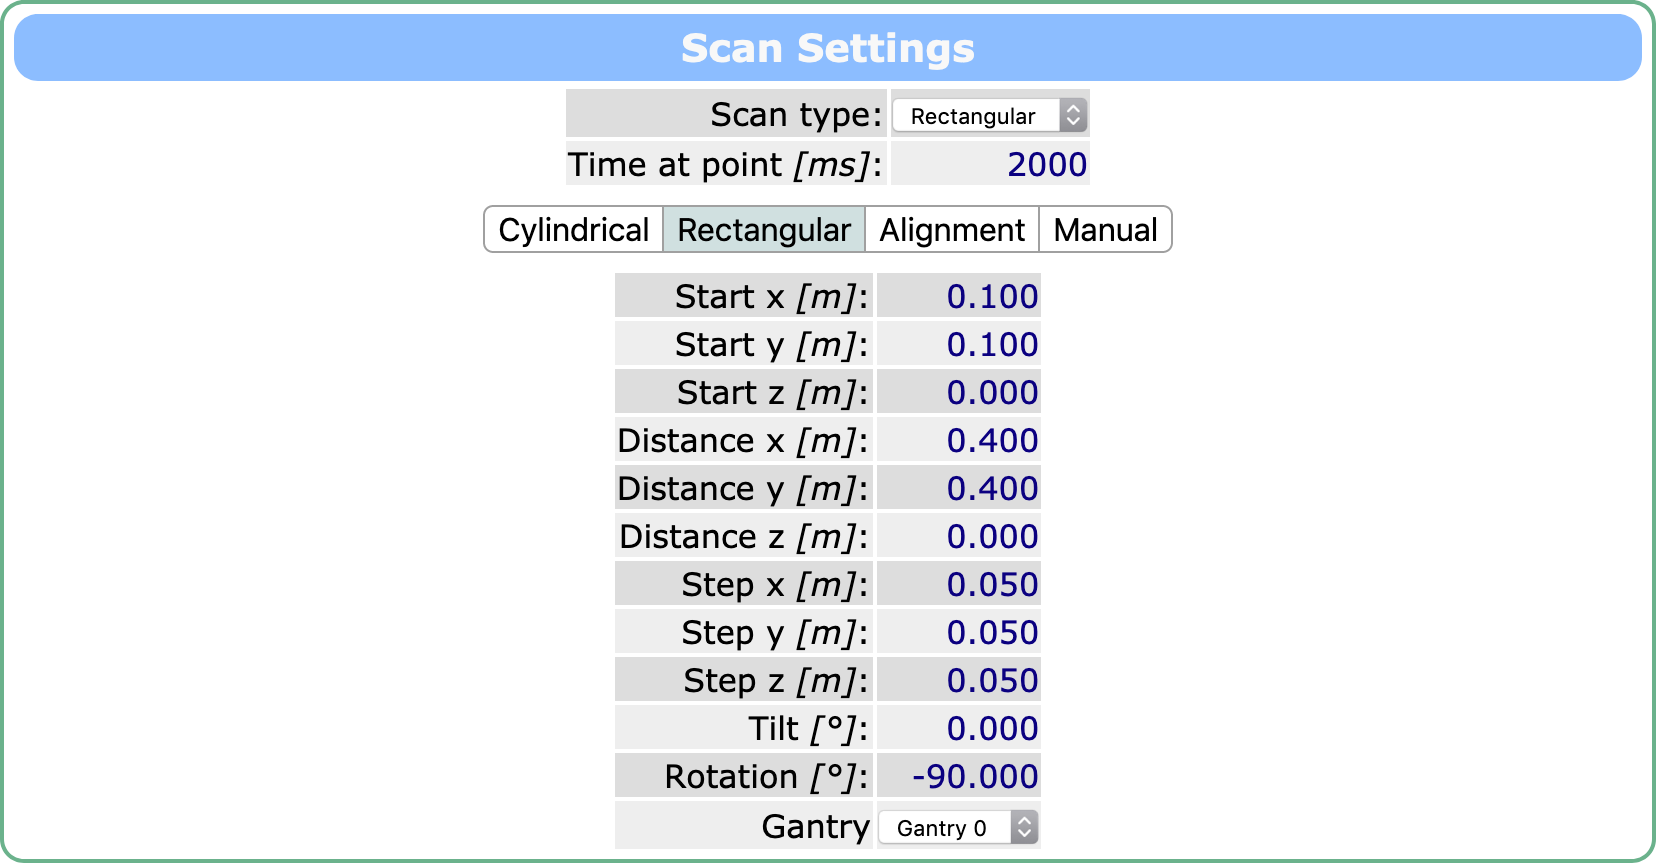
\includegraphics[width=\textwidth]{scanParams.png}
	\caption{The scan configuration page.\label{fig:scanParams}}
\end{figure}
\FloatBarrier


\subsubsection{Scan Preparations}

Before beginning such a scan, we must ensure (as in Section~\ref{singleData}) that the laser beam is powered and connected to the gantry which will be moved, the curtains are closed, and all equipment is properly powered as in Section~\ref{PowerUP}.


\subsubsection{Setting Up a Scan}

The process for setting up a scan is as follows

\begin{enumerate}
	
	\item Initialize gantries if the motors have been OFF or if you don't trust the positions for some reason.
	
	\item Make sure feSCAN frontend (Scan) is switched OFF
	
	\item Navigate to the \textbf{Scan} tab of the navigation tabs section (\ref{navTabs}).	
	
	\item Once in the Scan page, select Rectangular from the drop down list.
	
	\item Set the time duration to 3--6 s per scan point (6 seconds is the standard with old DAQ electronics, 3s is standard with the waveform digitizer)
	
	\item Define the scan volume:
			
			The length, width and height fields describe a rectangular volume relative to your initial position, i.e the bottom left vertex coordinate of the volume is the initial position. This rectangular volume will be stepped through according to the step sizes in a given direction, beginning with the provided initial position.
			
			The step size must be greater than or equal to 0.001 (metres). However, you can fix motion in a plane by setting either the length, width or height of the rectangular volume mentioned above to be equal to 0. If the L/W/H is set to 0, regardless of the step size the gantry will not move in that direction.
			
			\textbf{A note on step sizes:
				Full area 1 cm resolution scans (0.01) take around 4 hours to complete with 3s scan time.
				Full area 5 mm resolution scans (0.005) take around 12 hours to complete with 3s scan time, but are much more detailed.}
				
	\item Choose a rotation and tilt angle:
	
			(For general surface scans, with laser pointing straight down, the convention is -90 for both rotation and tilt). For non-vertical scans that use angles of incidence other than 90 degrees (normal) to the PMT, the angular offset from normal must be specified in the ScanSequence.cxx code with sub type 2 / Normal Incidence selected. Further details on ScanSequence.cxx are given in Section~\ref{scanScripts}.
	
	\item Choose a gantry to use:
	
			We only have the laser directed to one optical box, so pick either gantry 0 or gantry 1 (0 and 1 correspond to gantry 0 and gantry 1 respectively)
			
	\item Choose a sub type:
	
			Sub Type 0/Default specifies a regular vertical injection scan of the PMT. Sub Type 1/Monitor Reference Point is the same as Default but will scan a reference point periodically. The point and periodicity are specified in the ODB at 
			/Equipment/Scan/RectangularParams/MonitorPoint. Sub Type 2 specifies a normal incidence (or offset incidence) scan.
	
	\textbf{AFTER setting all scan settings above, switch ON the feSCAN frontend. If any settings change, you need to reset the frontend to reload the settings.}
	
	
\end{enumerate}


\subsubsection{Beginning the Scan}

Return to the main midptf status page (\ref{statusPage}), and click Start to execute the scan. A screen should pop up, prompting comments to describe the scan. Fill this in precisely. The scan should begin within a few seconds.

\subsubsection{Monitoring the Scan}

Check the messages or the midas.log to see whether there are any errors from feSCAN or whether there is more than one scan point specified. Otherwise there might be an error with the boundaries of the grid definition. The scan should now complete on its own. It is suggested to track the gantry positions to ensure that it is scanning properly by observing the gantryMove page as the scan is running.

The non-scanning gantry typically must move out of the way to allow the scanning gantry access to one half of the region, so do not be alarmed to see the other gantry moving from corner to corner. Though it is recommended to take test scans first without the PMT on to understand the quirks of the scanning algorithm.

\subsubsection{Ending a Scan}

Once the scan is running it can be left to finish on its own without worry. As a safety precaution, if there are no other scans planned in the immediate future, it would be wise to turn off the laser between scans. This can be done remotely or by turning the key on the laser itself to the OFF position. Also remember to reset feScan (restarting it) if you want to take a different scan region or use a different coordinate system.



\clearpage
\section{Data Analysis}

\subsection{Overview}\label{dataAnalysisFiles}

Analysis of measurements taken in the PTF is performed by analyzing data from ROOT files, a hierarchical data structure that is very efficient for processing event based data. If the option to write data to a file is selected at the start of a measurement, then a ROOT file will be automatically generated in the directory \textbf{/online/rootfiles/} on \textbf{midptf@midptf01}.

Previously, a single very large script was used for all of the analysis of data from the PTF. However, this file eventually grew very large and became difficult to make any changes to. So, a new library has been written which makes it very easy to make a new analysis script for a particular purpose. It (and its documentation) can be found in \href{https://bitbucket.org/ttriumfdaq/ptf-analysis-2}{this repository}.

Antiquated data analysis scripts (developed for use with scans completed with ADC and TDC modules) are located in:

\textbf{/online/src/analysis\_scripts/ADC\_Fitting\_Scripts}

\textbf{/online/src/analysis\_scripts/TDC\_Fitting\_Scripts}

\subsection{ROOT Analysis Package}

A combination of ROOT 5 and 6 are used in different places. For some programs on the midptf01 machine, ROOT 5 is used (the particular installation is v5.34/38, located at \texttt{/packages/root}). However, for the analysis ROOT 6 is used. Do note that there are incompatibilities between ROOT 5 and 6.

ROOT may not be installed on your local machine, and so it may need to be built first. You may also need to build a newer version of GCC in order to build ROOT, depending on the machine.
	
Different people have different methods on doing this, so ask around to find a method that works for you.

\subsection{Navigating the ROOT File}

The structure of the ROOT file that is generated when data is taken is hierarchical, with a primary \emph{Tree} composed of \emph{Branches} which contain certain data values. Documentation for using ROOT can be found in the \href{https://root.cern.ch/guides/users-guide}{ROOT User's Guide}. To gain familiarity with the file structure it is suggested to use the interactive command line environment as well as the graphical interface started by starting an instance of \emph{TBrowser} (i.e try typing \texttt{TBrowser B} in the ROOT command line to start).

Please see the documentation \href{https://bitbucket.org/ttriumfdaq/ptf-analysis-2}{here} for how to use the wrapper, which takes care of all of the above automatically.

\subsubsection{Analysis Method and ROOT File Structure Overview}

Analysis of the ROOT files occurs point by point for each position on the PMT.\@ The structure of the ROOT file is conducive to this type of analysis. Each root file contains a number of entries, each corresponding to a single PMT position. At each entry, there are a series of branches, each containing different data fields from the run (positional data, waveforms, etc).

Iterating over each entry and using pointers allows memory-efficient reading of the ROOT file. For each position (entry), the local script variable addresses are set to the addresses of the branch variables in the ROOT file. This allows very fast data analysis without the massive data transfer overhead.

There are three main types of data that are found in the ROOT files produced with the PTF.\@ Some data fields only contain a single value (for example the x position or y position of a point in the PMT scan). However, the data fields that are of more interest, such as the older ADC and TDC data fields and the new waveform digitizer data fields make use of arrays to efficiently store information. In the case of ADC and TDC data, the arrays were one dimensional, containing a single column with each entry being a different measurement or sample over a short (100ns) time window. The digitizer data is contained in a 2 dimensional array, with many rows, each containing the waveform from the PMT for a specific laser pulse. Iteration over these arrays and the subsequent analysis of the data contained in them is the primary method used to extract PMT response characteristics.

\subsection{Integrative Data Analysis}

Prior to the installation of the waveform digitizer, integrative methods were used to assess PMT response. These included a total charge measurement, as well as a Timing Difference distribution between a pulse from the monitor PMT inside the gantry and the main 20'' PMT.\@ These analysis methods can still be used, however the Charge and Time spectra are now created by analyzing the waveform digitizer data instead of being generated by individual modules.

\subsubsection{ADC (Charge) Spectrum Analysis}

Measurement of the response of the PMT at a point is primarily performed by analyzing the ADC Spectrum from the PMT at that point. An ADC Spectrum is a histogram representation of the recorded charge produced from a series of single photons incident to the PMT photocathode. The horizontal axis is a series of bins proportional to the measured charge over a time interval, and the vertical axis is a count of the events in each bin. \textbf{Note: Some charge spectra may appear `flipped' about the pedestal. This is because the PMT produces a negative pulse.}

\FloatBarrier

\begin{figure}[!htpb]\centering	
	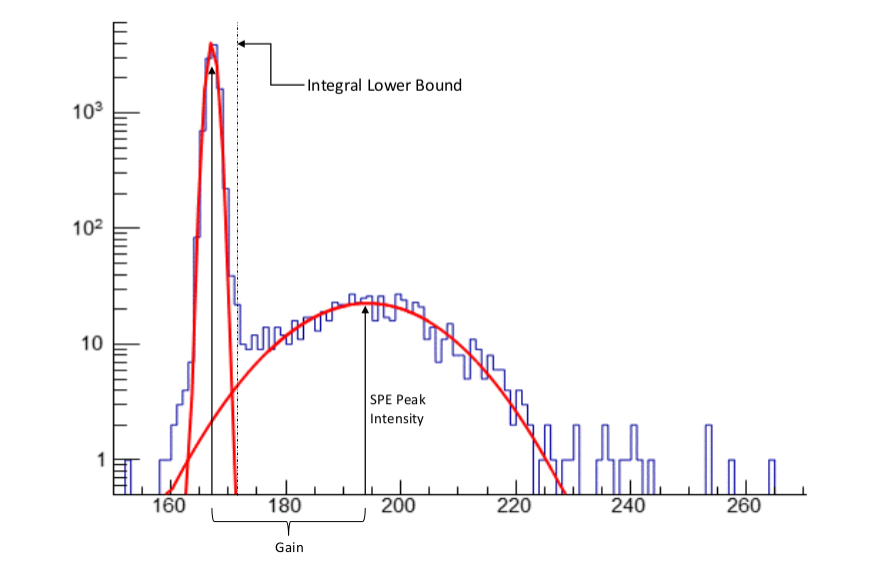
\includegraphics[width=\picwidth]{images/adcSpectrum}
	\caption{Labelled Example ADC Spectrum\label{adcSpectrum}}
\end{figure}

\FloatBarrier

There are two primary components of an ADC Spectrum. The \textbf{pedestal} distribution is a measurement of the PMT signal when there is no incident photon. The pedestal is usually a very narrow tall peak that dominates the overall count of the spectrum. Separate from the pedestal is the \textbf{photoelectron peak distribution}, which is a distribution composed of any signal which does not fall into the narrow pedestal band. Events in this distribution are produced by incident photons or a background counting rate which must be corrected for.

\subsubsection{Terminology and Definitions}

Analysis of the spectrum is performed by fitting both the \textbf{pedestal} and \textbf{photoelectron peak} distributions with Gaussian functions $g_p(q)$ and $g_s(q)$ respectively, and extracting data from the fit parameters. For an individual gaussian function, the fit parameters are:

\begin{description}
	
\item[\textbf{Sigma}]

The spread of the gaussian function in charge. $\sigma$

\item[\textbf{Constant}]

The height of the gaussian function in counts. $\alpha$

\item[\textbf{Mean}] The mean value of the gaussian function in charge. $\mu$

\end{description}

From the fit parameters, a variety of PMT properties can be calculated for a single point on the surface.

\begin{description}
	\item[\textbf{Gain}] Gain is defined as the magnitude of the measured charge as a multiple of the charge on an electron $e$. In terms of fit parameters, it is mathematically expressed as: \[\mu_{measured} = \mu_s - \mu_p \]
	\item[\textbf{SPE Peak Intensity}] The local maximum of the fitted gaussian (unitless). In terms of fit parameters, it is expressed as: \[ \alpha \]
	\item[\textbf{Peak To Valley Ratio}] The peak to valley ratio is a measure of how ``well-defined'' the photoelectron peak is. It is calculated as the ratio between the SPE peak intensity and the height of the valley between $g_s(q)$ and $g_p(q)$. Mathematically this is expressed as: \[\phi = \frac{\alpha}{\min(\{|g_s(q)| - |g_p(q)|: q \in (\mu_p, \mu_s)\})} \]
	\item[\textbf{Charge Resolution}] Charge resolution is a measure of how discernible a single electron peak is in the charge spectrum. It is defined as the ratio between the spread of the fitted gaussian to the distance between the mean of the photoelectron peak and the pedestal mean, expressed mathematically as: \[\frac{\sigma}{\mu_{measured}}\]

\end{description}

It is possible to measure additional parameters beyond those listed, and the calculation and definition of these parameters should be added in with the parameters above for reference.


\subsubsection{Time Distribution Analysis}

Timing data for the PMT is acquired by measuring the difference in time between some reference pulse (either externally generated or from the monitor PMT) and the time at which the PMT pulse crosses a certain voltage threshold (~3.5mV in our case). By plotting the distribution of the time differences, a skewed gaussian can be obtained and fitted, and extracting the parameter sigma of the fitted Gaussian provides a measurement of the \textbf{Transit Time Spread (TTS)} for that position on the PMT.

\FloatBarrier

\begin{figure}[!htpb]\centering
	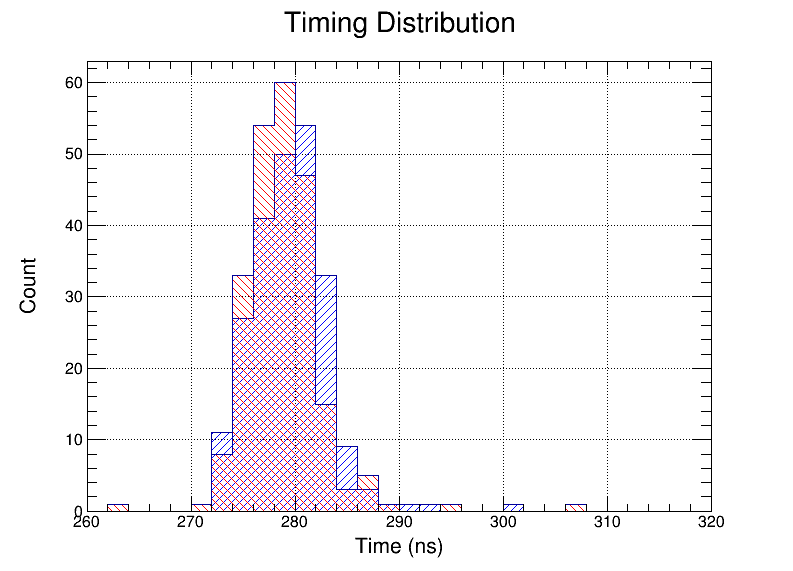
\includegraphics[width=\picwidth]{images/tdcSpectrum.png}
	\caption{Labelled Example TDC Spectrum\label{tdcSpectrum}}
\end{figure}

\FloatBarrier

Figure~\ref{tdcSpectrum} depicts a sample Transit Time Distribution, with the blue showing the raw peak time differences and the red overlay showing the difference between the mean of the waveform fits.

The importance of obtaining an accurate transit time spread measurement is related to the ability to identify the location of an event in the Large Water Cherenkov detector at SuperK. If the transit time spread for a single PMT is known, and independent of the absolute transit time, the uncertainty on the time of flight of a photon incident to that PMT is also known. Improving (reducing) the transit time spread therefore allows more accurate measurement of the position of an event within the detector.

\clearpage

\subsection{Waveform Digitizer (Low Level) Analysis}



Installation of the waveform digitizer (CAEN V1730 Model) to the PMT allows simultaneous collection of charge and timing data based on analysis of individual waveforms for each PMT pulse.

\subsubsection{Sample Waveform and Analysis}\label{waveformAnalysis}

Figure~\ref{sampleWav} shows a sample waveform obtained from the PMT with the waveform digitizer. The PMT pulse is clearly seen and obviously separate from the noise. For each pulse sent to the laser, there is a time window of 400 ns (200 samples at 500MS/s) captured with the digitizer which contains both the reference pulse and the PMT pulse. This data is written to a MIDAS file and then converted to a ROOT file, which produces histograms of the waveforms for the 70 samples around both the reference pulse and the PMT pulse (they are currently offset by 130 samples, with the reference pulse occurring earlier in time).

\FloatBarrier

\begin{figure}[!htpb]\centering	
	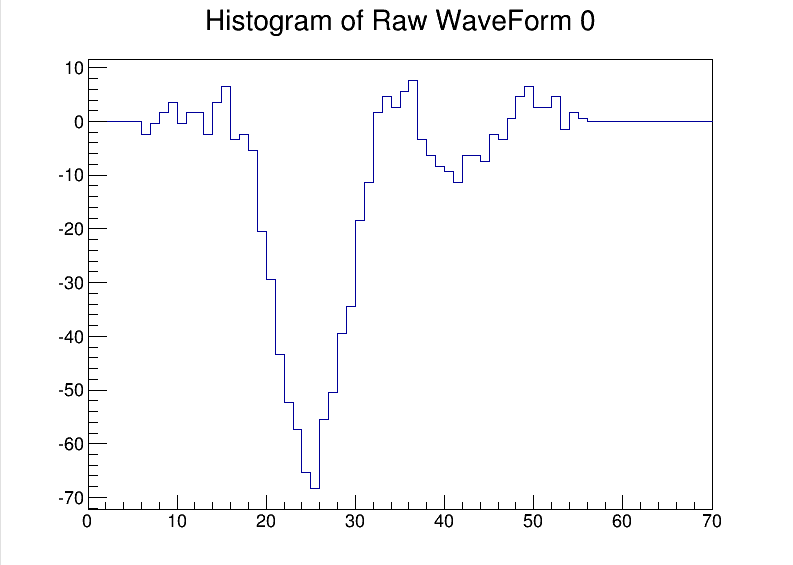
\includegraphics[width=\picwidth]{images/sampleWav.png}
	\caption{Example PMT Pulse Waveform\label{sampleWav}}
\end{figure}

\FloatBarrier

\begin{figure}[!htpb]\centering	
	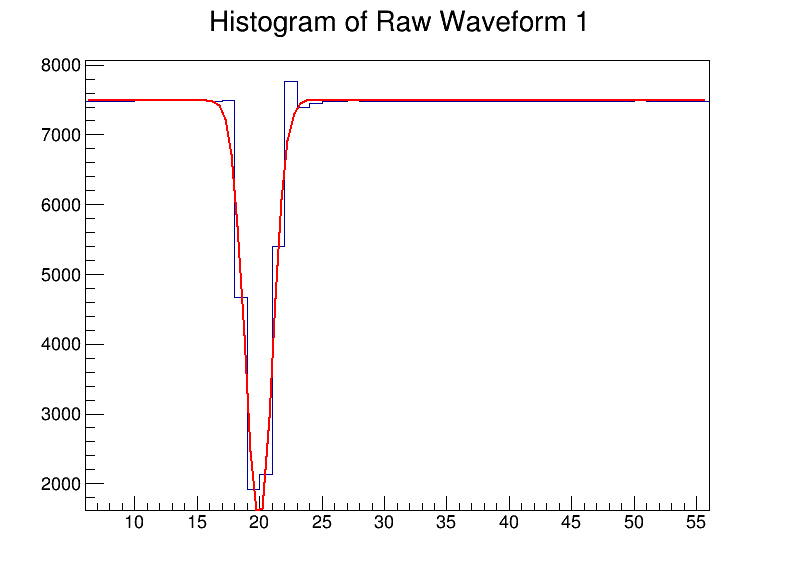
\includegraphics[width=\picwidth]{images/refWav.png}
	\caption{Example Reference Pulse Waveform\label{refWav}}
\end{figure}

\FloatBarrier

Simple gaussian functions (written in digiAna\_v2.cxx code) are fitted to the pulses to provide more accurate measures of pulse width and time than that available using only the histograms themselves. The integral of these fitted waveforms (for the PMT pulse) provides a measurement of the theoretical PMT charge which helps to improve the understanding of PMT response.

\subsection{Data Analysis Scripts}

To perform the analysis of the charge spectrum, the ROOT files which are mentioned in Section~\ref{dataAnalysisFiles} must be analyzed. There are a variety of script files, and each has a well-defined function:

\subsubsection{Old Analysis Scripts}

The following scripts are for analysis of runs taken prior to Run 2769 (runs taken using TDC or ADC).

Scripts contained in \textbf{online/src/analysis\_scripts/ADC\_Fitting\_Scripts} directory:

\begin{enumerate}
	
	\item[\textbf{FitAnalysis.C}] This script takes a ROOT file containing scan data taken at 1cm resolution and creates an X-Y map of a given parameter, in addition to taking statistics of various parameters at each (x,y) point. These are output as ROOT figures, which can be saved as .pdf files.
	\item[\textbf{Parameter1cm.C}] This script largely performs the same function as FitAnalysis1cm.C however is useful for extracting different parameters from the run with minimal fitting (i.e total number of points, time spent per point, magnetic field etc.).
	
\end{enumerate}

% Scripts contained in \textbf{online/src/analysis\_scripts/MAG\_FIELD\_SCRIPTS/} directory:

% \begin{enumerate}

% 	\item[\textbf{magFieldPlotClean.py}] Takes a ROOT file containing 3d scan data taken at a resolution and range specified (by editing the limits in the script) and generates X-Y, Y-Z, and X-Z plane maps of the magnetic field strength in all directions. This is a python script that requires the matplotlib and numpy Python packages to work properly. Preferred Python environment is the Anaconda Python 2.7 distribution.
% 	\item[\textbf{magFieldPlot.py}] Similar functionality to \textbf{magFieldPlotClean.py} however provides less polished figures unsuitable for external use. Presents more data in the quiver plot format than the clean version of the script.

% \end{enumerate}

As a note, to change between extracted parameters in the FitAnalysis and Parameter scripts, code must be changed in the section which writes data to the final displayed histogram. This is fairly straightforward, but is a bit technical to include in this reference manual.

% \subsubsection{Waveform-based Analysis Scripts}

% The following scripts are for analysis of runs taken after Run 2769 (runs taken using the waveform digitizer) and are contained in the directory: \textbf{online/src/analysis\_scripts/wv\_digi\_analysis\_scripts/}.

% \textbf{Note: Run 2965 is a very good script for testing data analysis. Run 3615 is also good as it is the most recent high resolution full compensation scan.}

% \begin{enumerate}
	
% 	\item [\textbf{digiAna\_v3.cxx}] This script takes a ROOT file containing scan data taken at some resolution and creates an X-Y map of a given parameter, in addition to taking statistics of various parameters at each (x,y) point. These are output as ROOT figures, which can be saved as .pdf files. This script iterates through each point on the PMT and analyzes all waveforms at that point to produce charge and time spectra which can then be used to extract a variety of parameters which describe the response of the PMT. As the analysis progresses various spectra are output to canvases including the final X-Y maps, which then have to be saved manually. This script has since been superseded by \textbf{digiAna\_v4.cxx}. However the v3 script is already set up to observe the raw waveforms during analysis among other spectra, which may have niche uses for testing.

% 	\item [\textbf{digiAna\_v4.cxx}] This functions the same as \textbf{v3} but with increased convenience as it saves every ADC and TDC spectra during analysis, in addition to the post-analysis plots, in a ROOT file.

% 	\item [\textbf{histogramViewer.cxx}] The nature of the ROOT TBrowser means that after running \textbf{digiAna\_v4.cxx}, the resultant plots may have inconsistent color styles. This script remedies that by reading in a ROOT file, making copies of whatever data is specified, and outputs them in a pre-set T2K-standard color style. Other operations can also be performed on these histograms (i.e: dividing out double binning if the original histogram did not have that operation applied).

% \end{enumerate}

% As a note, the X-Y maps in the analysis scripts have different sizes and binning to correspond with the resolution of a run - typically 2cm, 1cm, and 5mm. Presently you must change between these resolutions by commenting.

\clearpage
\subsection{Analysis Guidelines and Final Notes}

Performing analysis of the PMT data using the scripts above is rather straightforward, however there are a few general guidelines which are important to follow for consistency and usability of the generated results.

\begin{itemize}
	\item Preferred format for figure generation is a \texttt{.pdf} or a \texttt{.png} file.
	\item Once generated, it is wise to save the figure files into an obvious directory named appropriately for the measurement which they describe.
	\item Any changes to the scripts which are tested and verified to work well are to be pushed up to the git repository hosted at Bitbucket, with a relevant and descriptive commit message.
	\item Images produced by a script should \emph{not} be added to version control. See \href{https://git-scm.com/docs/gitignore}{here} for information on automatically excluding files from git.
	\item If you are new to the Linux development environment, it is very important to learn a command-line editor such as \textbf{emacs} or \textbf{vim}. These make small changes very easy, especially when working remotely.
	\item Any time data of special significance is generated, either as a reference figure or a final measurement result, the figures should be sent around to the PTF collaborators via email and an E-Log added describing the significance of the measurements.
\end{itemize}

\clearpage

\section{Magnetic Field Compensation \& Control}\label{sec:magField}

The magnetic field has a large and important effect on PMTs. As the PTF is near the cyclotron, understanding and controlling the field is essential for good results when scanning PMTs. Note that the cyclotron is off from the end of December until April every year for maintenance, and so the field is very different during this period.

The magnetic field inside the PTF is very complicated. The passive shielding component (G-Iron) creates hysteresis in the field, as well as making the field dependent on coils one might not expect. For example, the coils normal to $\hat{x}$ also have an effect on the $y$ and $z$ components of the field. The hysteresis is compensated for by a process called degaussing, which is explained below.

Characterizing this fully is a time-intensive process, hampered by many sources of noise in the field. Of major importance is the 52-ton crane used to move equipment inside the Meson Hall. It is large enough that its motion changes the magnetic field inside the PTF significantly. As such, it's generally best to do scans and calibration at night or over the weekend when the crane will not be moving.

The magnetometers used (``phidgets'') also have multiple sources of noise. They are temperature-sensitive, and as the room heats up and cools down their readings change by about 1mG. Some of the phidgets will jump between two distinct values, often separated by a few mG. Finally, there is a longer-period (on the order of a day) change in the readings of the phidgets, the source of which has not been identified.

The primary goal in controlling the field inside the PTF is to get the field as close to zero as possible throughout the entire area that the PMT is in. A secondary goal is to create a constant nonzero field across (for example, $\mathbf{B} = \left( 0, 0, 100\text{mG} \right)$) across the whole area in order to characterize the magnetic field dependence of the PMTs' responses.

\subsection{Degaussing}

Degaussing is the process used to counteract the path-dependence of the magnetic field inside the PTF.\@ Since every path that the coil current takes affects the field, we define a path that is regular enough to produce a consistent field. This is done by picking a value far from the desired voltage, and exponentially approaching the final value while alternating whether the current value is above or below. Eight steps of this process gives a field repeatable to within the sensitivity of the phidgets. Figure~\ref{fig:degauss} gives a visual explanation of the degauss process.

To calculate the proper voltages, the following formula is used: \(V(i) = V_t + {(-1)}^i c e^{-ik}\), where \(i\) is the step number, \(V_t\) is the target voltage and \(c\) and \(k\) are determined as follows. They are chosen such that they will produce the biggest range of voltages in the degauss without exceeding voltage limitations of the coils (15V for Coils 1 and 2, 8V for the rest) and to get within a certain voltage of the target voltage on step \(n\). This is done in the routine \texttt{degauss/degauss:exponential\_factors}. First it sets \(c = V_\text{max} - V_t\) and \(k = -e^{\Delta V_\text{min}} / n\). \(\Delta V_\text{min}\) is the difference in voltage we want on the penultimate step, and is controlled by the parameter \texttt{MIN\_V\_DIFF} in \texttt{degauss/degauss.hxx}. If this value would result in the voltage being set less than a minimum $V_\text{min}$ (controlled by \texttt{V\_LOW\_MARGIN}), $c$ is set to $\left(V_t - V_\text{min}\right) / e^{-k}$ instead.

When a repeatable field is desired it's very important to degauss, and not simply set the voltages/currents. Note that for a truly repeatable field, all six coils must run the process at the same time.

To degauss to a particular set of values, use the Coil Control page in MIDAS. In the section labelled ``Degauss'', set each of the final voltages and the number of steps to take (8 steps is recommended). Then, click ``Start Degauss''. This can take a minute or two to run.

\FloatBarrier
\begin{figure}[!htb]\centering
  \resizebox{\textwidth}{!}{%% Creator: Matplotlib, PGF backend
%%
%% To include the figure in your LaTeX document, write
%%   \input{<filename>.pgf}
%%
%% Make sure the required packages are loaded in your preamble
%%   \usepackage{pgf}
%%
%% Figures using additional raster images can only be included by \input if
%% they are in the same directory as the main LaTeX file. For loading figures
%% from other directories you can use the `import` package
%%   \usepackage{import}
%% and then include the figures with
%%   \import{<path to file>}{<filename>.pgf}
%%
%% Matplotlib used the following preamble
%%   \usepackage{fontspec}
%%   \setmainfont{texgyreadventor-regular.otf}[Path=/Library/Fonts/]
%%   \setsansfont{texgyrepagella-regular.otf}[Path=/Library/Fonts/]
%%   \setmonofont{DejaVuSansMono.ttf}[Path=/usr/local/lib/python3.7/site-packages/matplotlib/mpl-data/fonts/ttf/]
%%
\begingroup%
\makeatletter%
\begin{pgfpicture}%
\pgfpathrectangle{\pgfpointorigin}{\pgfqpoint{6.500000in}{3.200000in}}%
\pgfusepath{use as bounding box, clip}%
\begin{pgfscope}%
\pgfsetbuttcap%
\pgfsetmiterjoin%
\definecolor{currentfill}{rgb}{1.000000,1.000000,1.000000}%
\pgfsetfillcolor{currentfill}%
\pgfsetlinewidth{0.000000pt}%
\definecolor{currentstroke}{rgb}{1.000000,1.000000,1.000000}%
\pgfsetstrokecolor{currentstroke}%
\pgfsetdash{}{0pt}%
\pgfpathmoveto{\pgfqpoint{0.000000in}{0.000000in}}%
\pgfpathlineto{\pgfqpoint{6.500000in}{0.000000in}}%
\pgfpathlineto{\pgfqpoint{6.500000in}{3.200000in}}%
\pgfpathlineto{\pgfqpoint{0.000000in}{3.200000in}}%
\pgfpathclose%
\pgfusepath{fill}%
\end{pgfscope}%
\begin{pgfscope}%
\pgfsetbuttcap%
\pgfsetmiterjoin%
\definecolor{currentfill}{rgb}{1.000000,1.000000,1.000000}%
\pgfsetfillcolor{currentfill}%
\pgfsetlinewidth{0.000000pt}%
\definecolor{currentstroke}{rgb}{0.000000,0.000000,0.000000}%
\pgfsetstrokecolor{currentstroke}%
\pgfsetstrokeopacity{0.000000}%
\pgfsetdash{}{0pt}%
\pgfpathmoveto{\pgfqpoint{0.812500in}{0.400000in}}%
\pgfpathlineto{\pgfqpoint{5.850000in}{0.400000in}}%
\pgfpathlineto{\pgfqpoint{5.850000in}{2.816000in}}%
\pgfpathlineto{\pgfqpoint{0.812500in}{2.816000in}}%
\pgfpathclose%
\pgfusepath{fill}%
\end{pgfscope}%
\begin{pgfscope}%
\pgfsetbuttcap%
\pgfsetroundjoin%
\definecolor{currentfill}{rgb}{0.000000,0.000000,0.000000}%
\pgfsetfillcolor{currentfill}%
\pgfsetlinewidth{0.803000pt}%
\definecolor{currentstroke}{rgb}{0.000000,0.000000,0.000000}%
\pgfsetstrokecolor{currentstroke}%
\pgfsetdash{}{0pt}%
\pgfsys@defobject{currentmarker}{\pgfqpoint{0.000000in}{-0.048611in}}{\pgfqpoint{0.000000in}{0.000000in}}{%
\pgfpathmoveto{\pgfqpoint{0.000000in}{0.000000in}}%
\pgfpathlineto{\pgfqpoint{0.000000in}{-0.048611in}}%
\pgfusepath{stroke,fill}%
}%
\begin{pgfscope}%
\pgfsys@transformshift{1.849632in}{0.400000in}%
\pgfsys@useobject{currentmarker}{}%
\end{pgfscope}%
\end{pgfscope}%
\begin{pgfscope}%
\definecolor{textcolor}{rgb}{0.000000,0.000000,0.000000}%
\pgfsetstrokecolor{textcolor}%
\pgfsetfillcolor{textcolor}%
\pgftext[x=1.849632in,y=0.302778in,,top]{\color{textcolor}\sffamily\fontsize{10.000000}{12.000000}\selectfont 2}%
\end{pgfscope}%
\begin{pgfscope}%
\pgfsetbuttcap%
\pgfsetroundjoin%
\definecolor{currentfill}{rgb}{0.000000,0.000000,0.000000}%
\pgfsetfillcolor{currentfill}%
\pgfsetlinewidth{0.803000pt}%
\definecolor{currentstroke}{rgb}{0.000000,0.000000,0.000000}%
\pgfsetstrokecolor{currentstroke}%
\pgfsetdash{}{0pt}%
\pgfsys@defobject{currentmarker}{\pgfqpoint{0.000000in}{-0.048611in}}{\pgfqpoint{0.000000in}{0.000000in}}{%
\pgfpathmoveto{\pgfqpoint{0.000000in}{0.000000in}}%
\pgfpathlineto{\pgfqpoint{0.000000in}{-0.048611in}}%
\pgfusepath{stroke,fill}%
}%
\begin{pgfscope}%
\pgfsys@transformshift{2.927172in}{0.400000in}%
\pgfsys@useobject{currentmarker}{}%
\end{pgfscope}%
\end{pgfscope}%
\begin{pgfscope}%
\definecolor{textcolor}{rgb}{0.000000,0.000000,0.000000}%
\pgfsetstrokecolor{textcolor}%
\pgfsetfillcolor{textcolor}%
\pgftext[x=2.927172in,y=0.302778in,,top]{\color{textcolor}\sffamily\fontsize{10.000000}{12.000000}\selectfont 4}%
\end{pgfscope}%
\begin{pgfscope}%
\pgfsetbuttcap%
\pgfsetroundjoin%
\definecolor{currentfill}{rgb}{0.000000,0.000000,0.000000}%
\pgfsetfillcolor{currentfill}%
\pgfsetlinewidth{0.803000pt}%
\definecolor{currentstroke}{rgb}{0.000000,0.000000,0.000000}%
\pgfsetstrokecolor{currentstroke}%
\pgfsetdash{}{0pt}%
\pgfsys@defobject{currentmarker}{\pgfqpoint{0.000000in}{-0.048611in}}{\pgfqpoint{0.000000in}{0.000000in}}{%
\pgfpathmoveto{\pgfqpoint{0.000000in}{0.000000in}}%
\pgfpathlineto{\pgfqpoint{0.000000in}{-0.048611in}}%
\pgfusepath{stroke,fill}%
}%
\begin{pgfscope}%
\pgfsys@transformshift{4.004713in}{0.400000in}%
\pgfsys@useobject{currentmarker}{}%
\end{pgfscope}%
\end{pgfscope}%
\begin{pgfscope}%
\definecolor{textcolor}{rgb}{0.000000,0.000000,0.000000}%
\pgfsetstrokecolor{textcolor}%
\pgfsetfillcolor{textcolor}%
\pgftext[x=4.004713in,y=0.302778in,,top]{\color{textcolor}\sffamily\fontsize{10.000000}{12.000000}\selectfont 6}%
\end{pgfscope}%
\begin{pgfscope}%
\pgfsetbuttcap%
\pgfsetroundjoin%
\definecolor{currentfill}{rgb}{0.000000,0.000000,0.000000}%
\pgfsetfillcolor{currentfill}%
\pgfsetlinewidth{0.803000pt}%
\definecolor{currentstroke}{rgb}{0.000000,0.000000,0.000000}%
\pgfsetstrokecolor{currentstroke}%
\pgfsetdash{}{0pt}%
\pgfsys@defobject{currentmarker}{\pgfqpoint{0.000000in}{-0.048611in}}{\pgfqpoint{0.000000in}{0.000000in}}{%
\pgfpathmoveto{\pgfqpoint{0.000000in}{0.000000in}}%
\pgfpathlineto{\pgfqpoint{0.000000in}{-0.048611in}}%
\pgfusepath{stroke,fill}%
}%
\begin{pgfscope}%
\pgfsys@transformshift{5.082253in}{0.400000in}%
\pgfsys@useobject{currentmarker}{}%
\end{pgfscope}%
\end{pgfscope}%
\begin{pgfscope}%
\definecolor{textcolor}{rgb}{0.000000,0.000000,0.000000}%
\pgfsetstrokecolor{textcolor}%
\pgfsetfillcolor{textcolor}%
\pgftext[x=5.082253in,y=0.302778in,,top]{\color{textcolor}\sffamily\fontsize{10.000000}{12.000000}\selectfont 8}%
\end{pgfscope}%
\begin{pgfscope}%
\definecolor{textcolor}{rgb}{0.000000,0.000000,0.000000}%
\pgfsetstrokecolor{textcolor}%
\pgfsetfillcolor{textcolor}%
\pgftext[x=3.331250in,y=0.107361in,,top]{\color{textcolor}\sffamily\fontsize{10.000000}{12.000000}\selectfont Step}%
\end{pgfscope}%
\begin{pgfscope}%
\pgfsetbuttcap%
\pgfsetroundjoin%
\definecolor{currentfill}{rgb}{0.000000,0.000000,0.000000}%
\pgfsetfillcolor{currentfill}%
\pgfsetlinewidth{0.803000pt}%
\definecolor{currentstroke}{rgb}{0.000000,0.000000,0.000000}%
\pgfsetstrokecolor{currentstroke}%
\pgfsetdash{}{0pt}%
\pgfsys@defobject{currentmarker}{\pgfqpoint{-0.048611in}{0.000000in}}{\pgfqpoint{0.000000in}{0.000000in}}{%
\pgfpathmoveto{\pgfqpoint{0.000000in}{0.000000in}}%
\pgfpathlineto{\pgfqpoint{-0.048611in}{0.000000in}}%
\pgfusepath{stroke,fill}%
}%
\begin{pgfscope}%
\pgfsys@transformshift{0.812500in}{0.400000in}%
\pgfsys@useobject{currentmarker}{}%
\end{pgfscope}%
\end{pgfscope}%
\begin{pgfscope}%
\definecolor{textcolor}{rgb}{0.000000,0.000000,0.000000}%
\pgfsetstrokecolor{textcolor}%
\pgfsetfillcolor{textcolor}%
\pgftext[x=0.645833in,y=0.349583in,left,base]{\color{textcolor}\sffamily\fontsize{10.000000}{12.000000}\selectfont 0}%
\end{pgfscope}%
\begin{pgfscope}%
\pgfsetbuttcap%
\pgfsetroundjoin%
\definecolor{currentfill}{rgb}{0.000000,0.000000,0.000000}%
\pgfsetfillcolor{currentfill}%
\pgfsetlinewidth{0.803000pt}%
\definecolor{currentstroke}{rgb}{0.000000,0.000000,0.000000}%
\pgfsetstrokecolor{currentstroke}%
\pgfsetdash{}{0pt}%
\pgfsys@defobject{currentmarker}{\pgfqpoint{-0.048611in}{0.000000in}}{\pgfqpoint{0.000000in}{0.000000in}}{%
\pgfpathmoveto{\pgfqpoint{0.000000in}{0.000000in}}%
\pgfpathlineto{\pgfqpoint{-0.048611in}{0.000000in}}%
\pgfusepath{stroke,fill}%
}%
\begin{pgfscope}%
\pgfsys@transformshift{0.812500in}{0.989268in}%
\pgfsys@useobject{currentmarker}{}%
\end{pgfscope}%
\end{pgfscope}%
\begin{pgfscope}%
\definecolor{textcolor}{rgb}{0.000000,0.000000,0.000000}%
\pgfsetstrokecolor{textcolor}%
\pgfsetfillcolor{textcolor}%
\pgftext[x=0.645833in,y=0.938852in,left,base]{\color{textcolor}\sffamily\fontsize{10.000000}{12.000000}\selectfont 2}%
\end{pgfscope}%
\begin{pgfscope}%
\pgfsetbuttcap%
\pgfsetroundjoin%
\definecolor{currentfill}{rgb}{0.000000,0.000000,0.000000}%
\pgfsetfillcolor{currentfill}%
\pgfsetlinewidth{0.803000pt}%
\definecolor{currentstroke}{rgb}{0.000000,0.000000,0.000000}%
\pgfsetstrokecolor{currentstroke}%
\pgfsetdash{}{0pt}%
\pgfsys@defobject{currentmarker}{\pgfqpoint{-0.048611in}{0.000000in}}{\pgfqpoint{0.000000in}{0.000000in}}{%
\pgfpathmoveto{\pgfqpoint{0.000000in}{0.000000in}}%
\pgfpathlineto{\pgfqpoint{-0.048611in}{0.000000in}}%
\pgfusepath{stroke,fill}%
}%
\begin{pgfscope}%
\pgfsys@transformshift{0.812500in}{1.578537in}%
\pgfsys@useobject{currentmarker}{}%
\end{pgfscope}%
\end{pgfscope}%
\begin{pgfscope}%
\definecolor{textcolor}{rgb}{0.000000,0.000000,0.000000}%
\pgfsetstrokecolor{textcolor}%
\pgfsetfillcolor{textcolor}%
\pgftext[x=0.645833in,y=1.528120in,left,base]{\color{textcolor}\sffamily\fontsize{10.000000}{12.000000}\selectfont 4}%
\end{pgfscope}%
\begin{pgfscope}%
\pgfsetbuttcap%
\pgfsetroundjoin%
\definecolor{currentfill}{rgb}{0.000000,0.000000,0.000000}%
\pgfsetfillcolor{currentfill}%
\pgfsetlinewidth{0.803000pt}%
\definecolor{currentstroke}{rgb}{0.000000,0.000000,0.000000}%
\pgfsetstrokecolor{currentstroke}%
\pgfsetdash{}{0pt}%
\pgfsys@defobject{currentmarker}{\pgfqpoint{-0.048611in}{0.000000in}}{\pgfqpoint{0.000000in}{0.000000in}}{%
\pgfpathmoveto{\pgfqpoint{0.000000in}{0.000000in}}%
\pgfpathlineto{\pgfqpoint{-0.048611in}{0.000000in}}%
\pgfusepath{stroke,fill}%
}%
\begin{pgfscope}%
\pgfsys@transformshift{0.812500in}{2.167805in}%
\pgfsys@useobject{currentmarker}{}%
\end{pgfscope}%
\end{pgfscope}%
\begin{pgfscope}%
\definecolor{textcolor}{rgb}{0.000000,0.000000,0.000000}%
\pgfsetstrokecolor{textcolor}%
\pgfsetfillcolor{textcolor}%
\pgftext[x=0.645833in,y=2.117388in,left,base]{\color{textcolor}\sffamily\fontsize{10.000000}{12.000000}\selectfont 6}%
\end{pgfscope}%
\begin{pgfscope}%
\pgfsetbuttcap%
\pgfsetroundjoin%
\definecolor{currentfill}{rgb}{0.000000,0.000000,0.000000}%
\pgfsetfillcolor{currentfill}%
\pgfsetlinewidth{0.803000pt}%
\definecolor{currentstroke}{rgb}{0.000000,0.000000,0.000000}%
\pgfsetstrokecolor{currentstroke}%
\pgfsetdash{}{0pt}%
\pgfsys@defobject{currentmarker}{\pgfqpoint{-0.048611in}{0.000000in}}{\pgfqpoint{0.000000in}{0.000000in}}{%
\pgfpathmoveto{\pgfqpoint{0.000000in}{0.000000in}}%
\pgfpathlineto{\pgfqpoint{-0.048611in}{0.000000in}}%
\pgfusepath{stroke,fill}%
}%
\begin{pgfscope}%
\pgfsys@transformshift{0.812500in}{2.757073in}%
\pgfsys@useobject{currentmarker}{}%
\end{pgfscope}%
\end{pgfscope}%
\begin{pgfscope}%
\definecolor{textcolor}{rgb}{0.000000,0.000000,0.000000}%
\pgfsetstrokecolor{textcolor}%
\pgfsetfillcolor{textcolor}%
\pgftext[x=0.645833in,y=2.706657in,left,base]{\color{textcolor}\sffamily\fontsize{10.000000}{12.000000}\selectfont 8}%
\end{pgfscope}%
\begin{pgfscope}%
\definecolor{textcolor}{rgb}{0.000000,0.000000,0.000000}%
\pgfsetstrokecolor{textcolor}%
\pgfsetfillcolor{textcolor}%
\pgftext[x=0.590278in,y=1.608000in,,bottom,rotate=90.000000]{\color{textcolor}\sffamily\fontsize{10.000000}{12.000000}\selectfont Voltage}%
\end{pgfscope}%
\begin{pgfscope}%
\pgfpathrectangle{\pgfqpoint{0.812500in}{0.400000in}}{\pgfqpoint{5.037500in}{2.416000in}}%
\pgfusepath{clip}%
\pgfsetrectcap%
\pgfsetroundjoin%
\pgfsetlinewidth{1.505625pt}%
\definecolor{currentstroke}{rgb}{0.000000,0.000000,0.000000}%
\pgfsetstrokecolor{currentstroke}%
\pgfsetdash{}{0pt}%
\pgfpathmoveto{\pgfqpoint{1.041477in}{2.757073in}}%
\pgfpathlineto{\pgfqpoint{1.580247in}{2.757073in}}%
\pgfusepath{stroke}%
\end{pgfscope}%
\begin{pgfscope}%
\pgfpathrectangle{\pgfqpoint{0.812500in}{0.400000in}}{\pgfqpoint{5.037500in}{2.416000in}}%
\pgfusepath{clip}%
\pgfsetrectcap%
\pgfsetroundjoin%
\pgfsetlinewidth{1.505625pt}%
\definecolor{currentstroke}{rgb}{0.000000,0.000000,0.000000}%
\pgfsetstrokecolor{currentstroke}%
\pgfsetdash{}{0pt}%
\pgfpathmoveto{\pgfqpoint{1.580247in}{0.915797in}}%
\pgfpathlineto{\pgfqpoint{2.119017in}{0.915797in}}%
\pgfusepath{stroke}%
\end{pgfscope}%
\begin{pgfscope}%
\pgfpathrectangle{\pgfqpoint{0.812500in}{0.400000in}}{\pgfqpoint{5.037500in}{2.416000in}}%
\pgfusepath{clip}%
\pgfsetrectcap%
\pgfsetroundjoin%
\pgfsetlinewidth{1.505625pt}%
\definecolor{currentstroke}{rgb}{0.000000,0.000000,0.000000}%
\pgfsetstrokecolor{currentstroke}%
\pgfsetdash{}{0pt}%
\pgfpathmoveto{\pgfqpoint{2.119017in}{1.951223in}}%
\pgfpathlineto{\pgfqpoint{2.657787in}{1.951223in}}%
\pgfusepath{stroke}%
\end{pgfscope}%
\begin{pgfscope}%
\pgfpathrectangle{\pgfqpoint{0.812500in}{0.400000in}}{\pgfqpoint{5.037500in}{2.416000in}}%
\pgfusepath{clip}%
\pgfsetrectcap%
\pgfsetroundjoin%
\pgfsetlinewidth{1.505625pt}%
\definecolor{currentstroke}{rgb}{0.000000,0.000000,0.000000}%
\pgfsetstrokecolor{currentstroke}%
\pgfsetdash{}{0pt}%
\pgfpathmoveto{\pgfqpoint{2.657787in}{1.368960in}}%
\pgfpathlineto{\pgfqpoint{3.196557in}{1.368960in}}%
\pgfusepath{stroke}%
\end{pgfscope}%
\begin{pgfscope}%
\pgfpathrectangle{\pgfqpoint{0.812500in}{0.400000in}}{\pgfqpoint{5.037500in}{2.416000in}}%
\pgfusepath{clip}%
\pgfsetrectcap%
\pgfsetroundjoin%
\pgfsetlinewidth{1.505625pt}%
\definecolor{currentstroke}{rgb}{0.000000,0.000000,0.000000}%
\pgfsetstrokecolor{currentstroke}%
\pgfsetdash{}{0pt}%
\pgfpathmoveto{\pgfqpoint{3.196557in}{1.696390in}}%
\pgfpathlineto{\pgfqpoint{3.735328in}{1.696390in}}%
\pgfusepath{stroke}%
\end{pgfscope}%
\begin{pgfscope}%
\pgfpathrectangle{\pgfqpoint{0.812500in}{0.400000in}}{\pgfqpoint{5.037500in}{2.416000in}}%
\pgfusepath{clip}%
\pgfsetrectcap%
\pgfsetroundjoin%
\pgfsetlinewidth{1.505625pt}%
\definecolor{currentstroke}{rgb}{0.000000,0.000000,0.000000}%
\pgfsetstrokecolor{currentstroke}%
\pgfsetdash{}{0pt}%
\pgfpathmoveto{\pgfqpoint{3.735328in}{1.512263in}}%
\pgfpathlineto{\pgfqpoint{4.274098in}{1.512263in}}%
\pgfusepath{stroke}%
\end{pgfscope}%
\begin{pgfscope}%
\pgfpathrectangle{\pgfqpoint{0.812500in}{0.400000in}}{\pgfqpoint{5.037500in}{2.416000in}}%
\pgfusepath{clip}%
\pgfsetrectcap%
\pgfsetroundjoin%
\pgfsetlinewidth{1.505625pt}%
\definecolor{currentstroke}{rgb}{0.000000,0.000000,0.000000}%
\pgfsetstrokecolor{currentstroke}%
\pgfsetdash{}{0pt}%
\pgfpathmoveto{\pgfqpoint{4.274098in}{1.615805in}}%
\pgfpathlineto{\pgfqpoint{4.812868in}{1.615805in}}%
\pgfusepath{stroke}%
\end{pgfscope}%
\begin{pgfscope}%
\pgfpathrectangle{\pgfqpoint{0.812500in}{0.400000in}}{\pgfqpoint{5.037500in}{2.416000in}}%
\pgfusepath{clip}%
\pgfsetrectcap%
\pgfsetroundjoin%
\pgfsetlinewidth{1.505625pt}%
\definecolor{currentstroke}{rgb}{0.000000,0.000000,0.000000}%
\pgfsetstrokecolor{currentstroke}%
\pgfsetdash{}{0pt}%
\pgfpathmoveto{\pgfqpoint{4.812868in}{1.557579in}}%
\pgfpathlineto{\pgfqpoint{5.351638in}{1.557579in}}%
\pgfusepath{stroke}%
\end{pgfscope}%
\begin{pgfscope}%
\pgfpathrectangle{\pgfqpoint{0.812500in}{0.400000in}}{\pgfqpoint{5.037500in}{2.416000in}}%
\pgfusepath{clip}%
\pgfsetbuttcap%
\pgfsetroundjoin%
\pgfsetlinewidth{1.003750pt}%
\definecolor{currentstroke}{rgb}{0.000000,0.000000,0.000000}%
\pgfsetstrokecolor{currentstroke}%
\pgfsetdash{{3.700000pt}{1.600000pt}}{0.000000pt}%
\pgfpathmoveto{\pgfqpoint{1.310862in}{1.578537in}}%
\pgfpathlineto{\pgfqpoint{5.621023in}{1.578537in}}%
\pgfusepath{stroke}%
\end{pgfscope}%
\begin{pgfscope}%
\pgfsetrectcap%
\pgfsetmiterjoin%
\pgfsetlinewidth{0.803000pt}%
\definecolor{currentstroke}{rgb}{0.000000,0.000000,0.000000}%
\pgfsetstrokecolor{currentstroke}%
\pgfsetdash{}{0pt}%
\pgfpathmoveto{\pgfqpoint{0.812500in}{0.400000in}}%
\pgfpathlineto{\pgfqpoint{0.812500in}{2.816000in}}%
\pgfusepath{stroke}%
\end{pgfscope}%
\begin{pgfscope}%
\pgfsetrectcap%
\pgfsetmiterjoin%
\pgfsetlinewidth{0.803000pt}%
\definecolor{currentstroke}{rgb}{0.000000,0.000000,0.000000}%
\pgfsetstrokecolor{currentstroke}%
\pgfsetdash{}{0pt}%
\pgfpathmoveto{\pgfqpoint{5.850000in}{0.400000in}}%
\pgfpathlineto{\pgfqpoint{5.850000in}{2.816000in}}%
\pgfusepath{stroke}%
\end{pgfscope}%
\begin{pgfscope}%
\pgfsetrectcap%
\pgfsetmiterjoin%
\pgfsetlinewidth{0.803000pt}%
\definecolor{currentstroke}{rgb}{0.000000,0.000000,0.000000}%
\pgfsetstrokecolor{currentstroke}%
\pgfsetdash{}{0pt}%
\pgfpathmoveto{\pgfqpoint{0.812500in}{0.400000in}}%
\pgfpathlineto{\pgfqpoint{5.850000in}{0.400000in}}%
\pgfusepath{stroke}%
\end{pgfscope}%
\begin{pgfscope}%
\pgfsetrectcap%
\pgfsetmiterjoin%
\pgfsetlinewidth{0.803000pt}%
\definecolor{currentstroke}{rgb}{0.000000,0.000000,0.000000}%
\pgfsetstrokecolor{currentstroke}%
\pgfsetdash{}{0pt}%
\pgfpathmoveto{\pgfqpoint{0.812500in}{2.816000in}}%
\pgfpathlineto{\pgfqpoint{5.850000in}{2.816000in}}%
\pgfusepath{stroke}%
\end{pgfscope}%
\end{pgfpicture}%
\makeatother%
\endgroup%
}
  \caption{An example of a degauss with eight steps.\label{fig:degauss}}
\end{figure}
\FloatBarrier

\subsection{Calibrating the Field}

Calibration is an iterative process due to the complexity of the field. At each iteration, there are two steps which must be done: zero the field for a particular dimension, and then remove the field differential in that dimension. Each iteration should pick a new dimension to zero. This will bring the field closer and closer to fully compensated.

Simply scanning all the possible voltages is not feasible. Even scanning every combination of 10 sample voltages for each coil would take approximately 60 years ($6^{10} \cdot 30\text{s}$), and to verify the differential is zero requires doing a regular scan of the PTF which would add significantly more time. This estimate does not take into account time lost due to the crane moving or time lost from cyclotron shutdowns.

\subsubsection{Zeroing a Dimension}

To find a zero value for a particular dimension, first attach an additional phidget to Gantry 0 as pictured in Figure~\ref{fig:gantryPositions}. This allows measuring over more of the volume of the PMT.

\FloatBarrier
\begin{figure}[htb!]\centering
  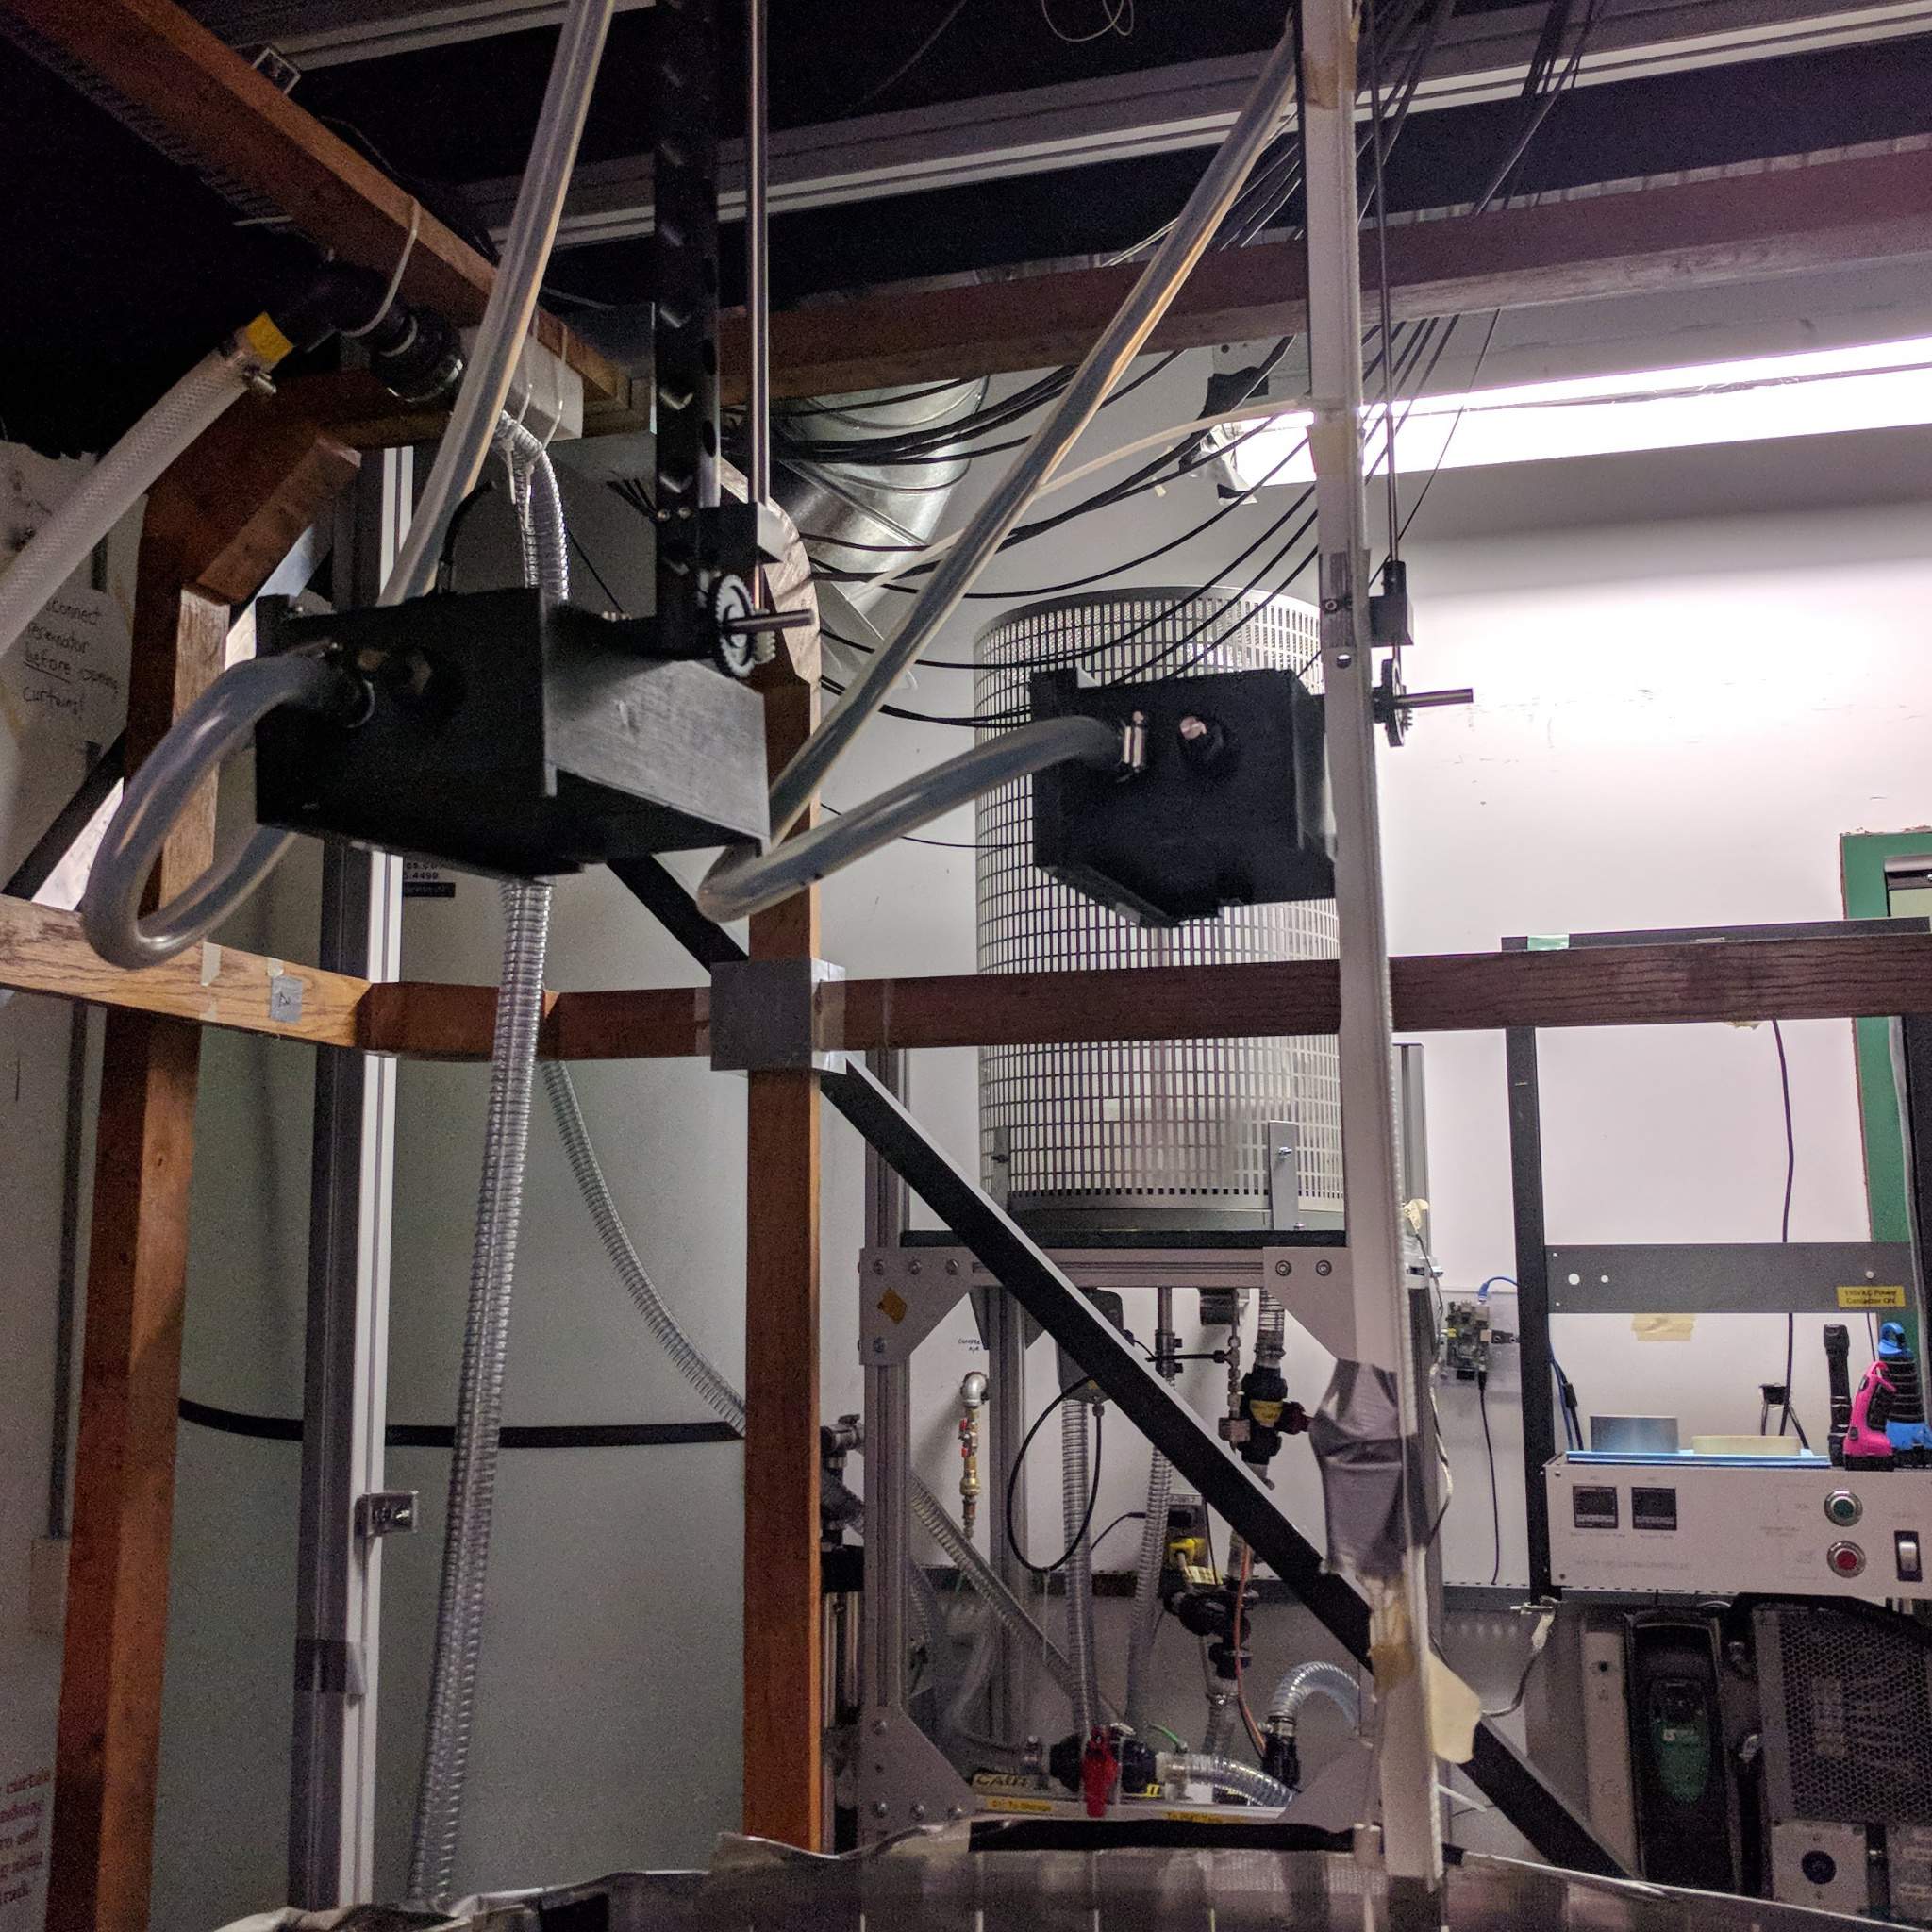
\includegraphics[width=0.325\textwidth]{images/gantriesBehind.jpg}
  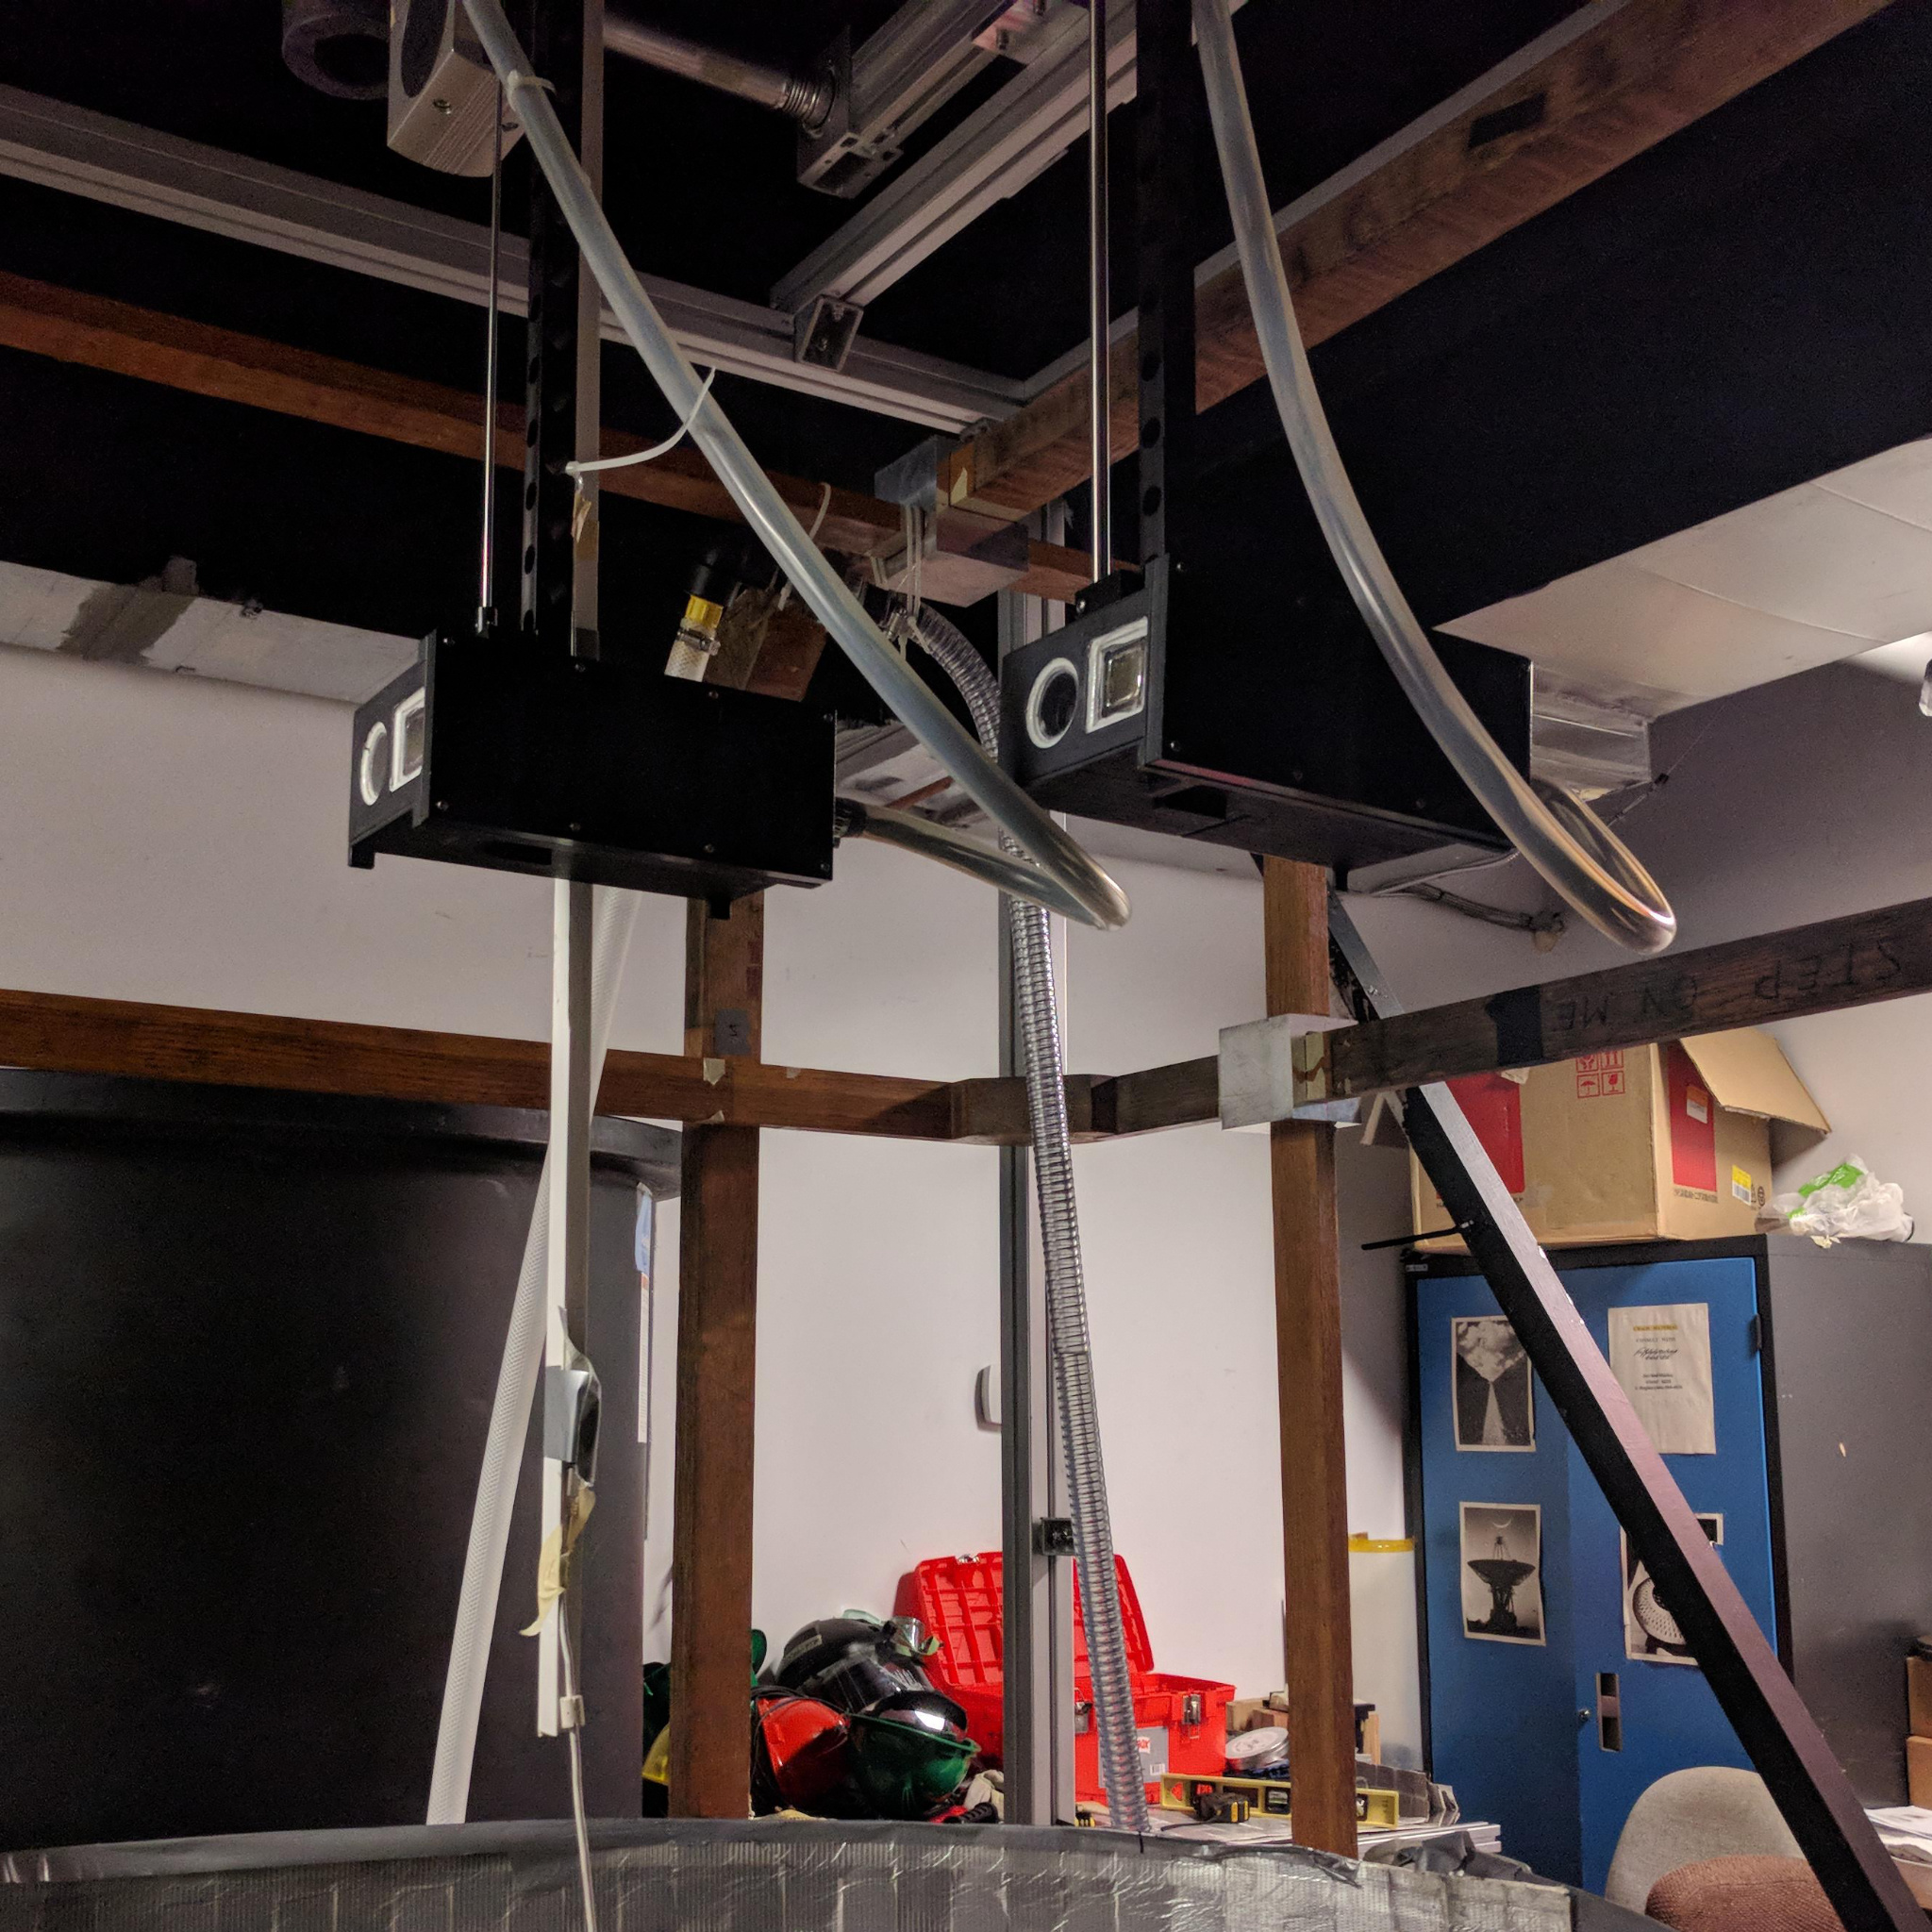
\includegraphics[width=0.325\textwidth]{images/gantriesSide.jpg}
  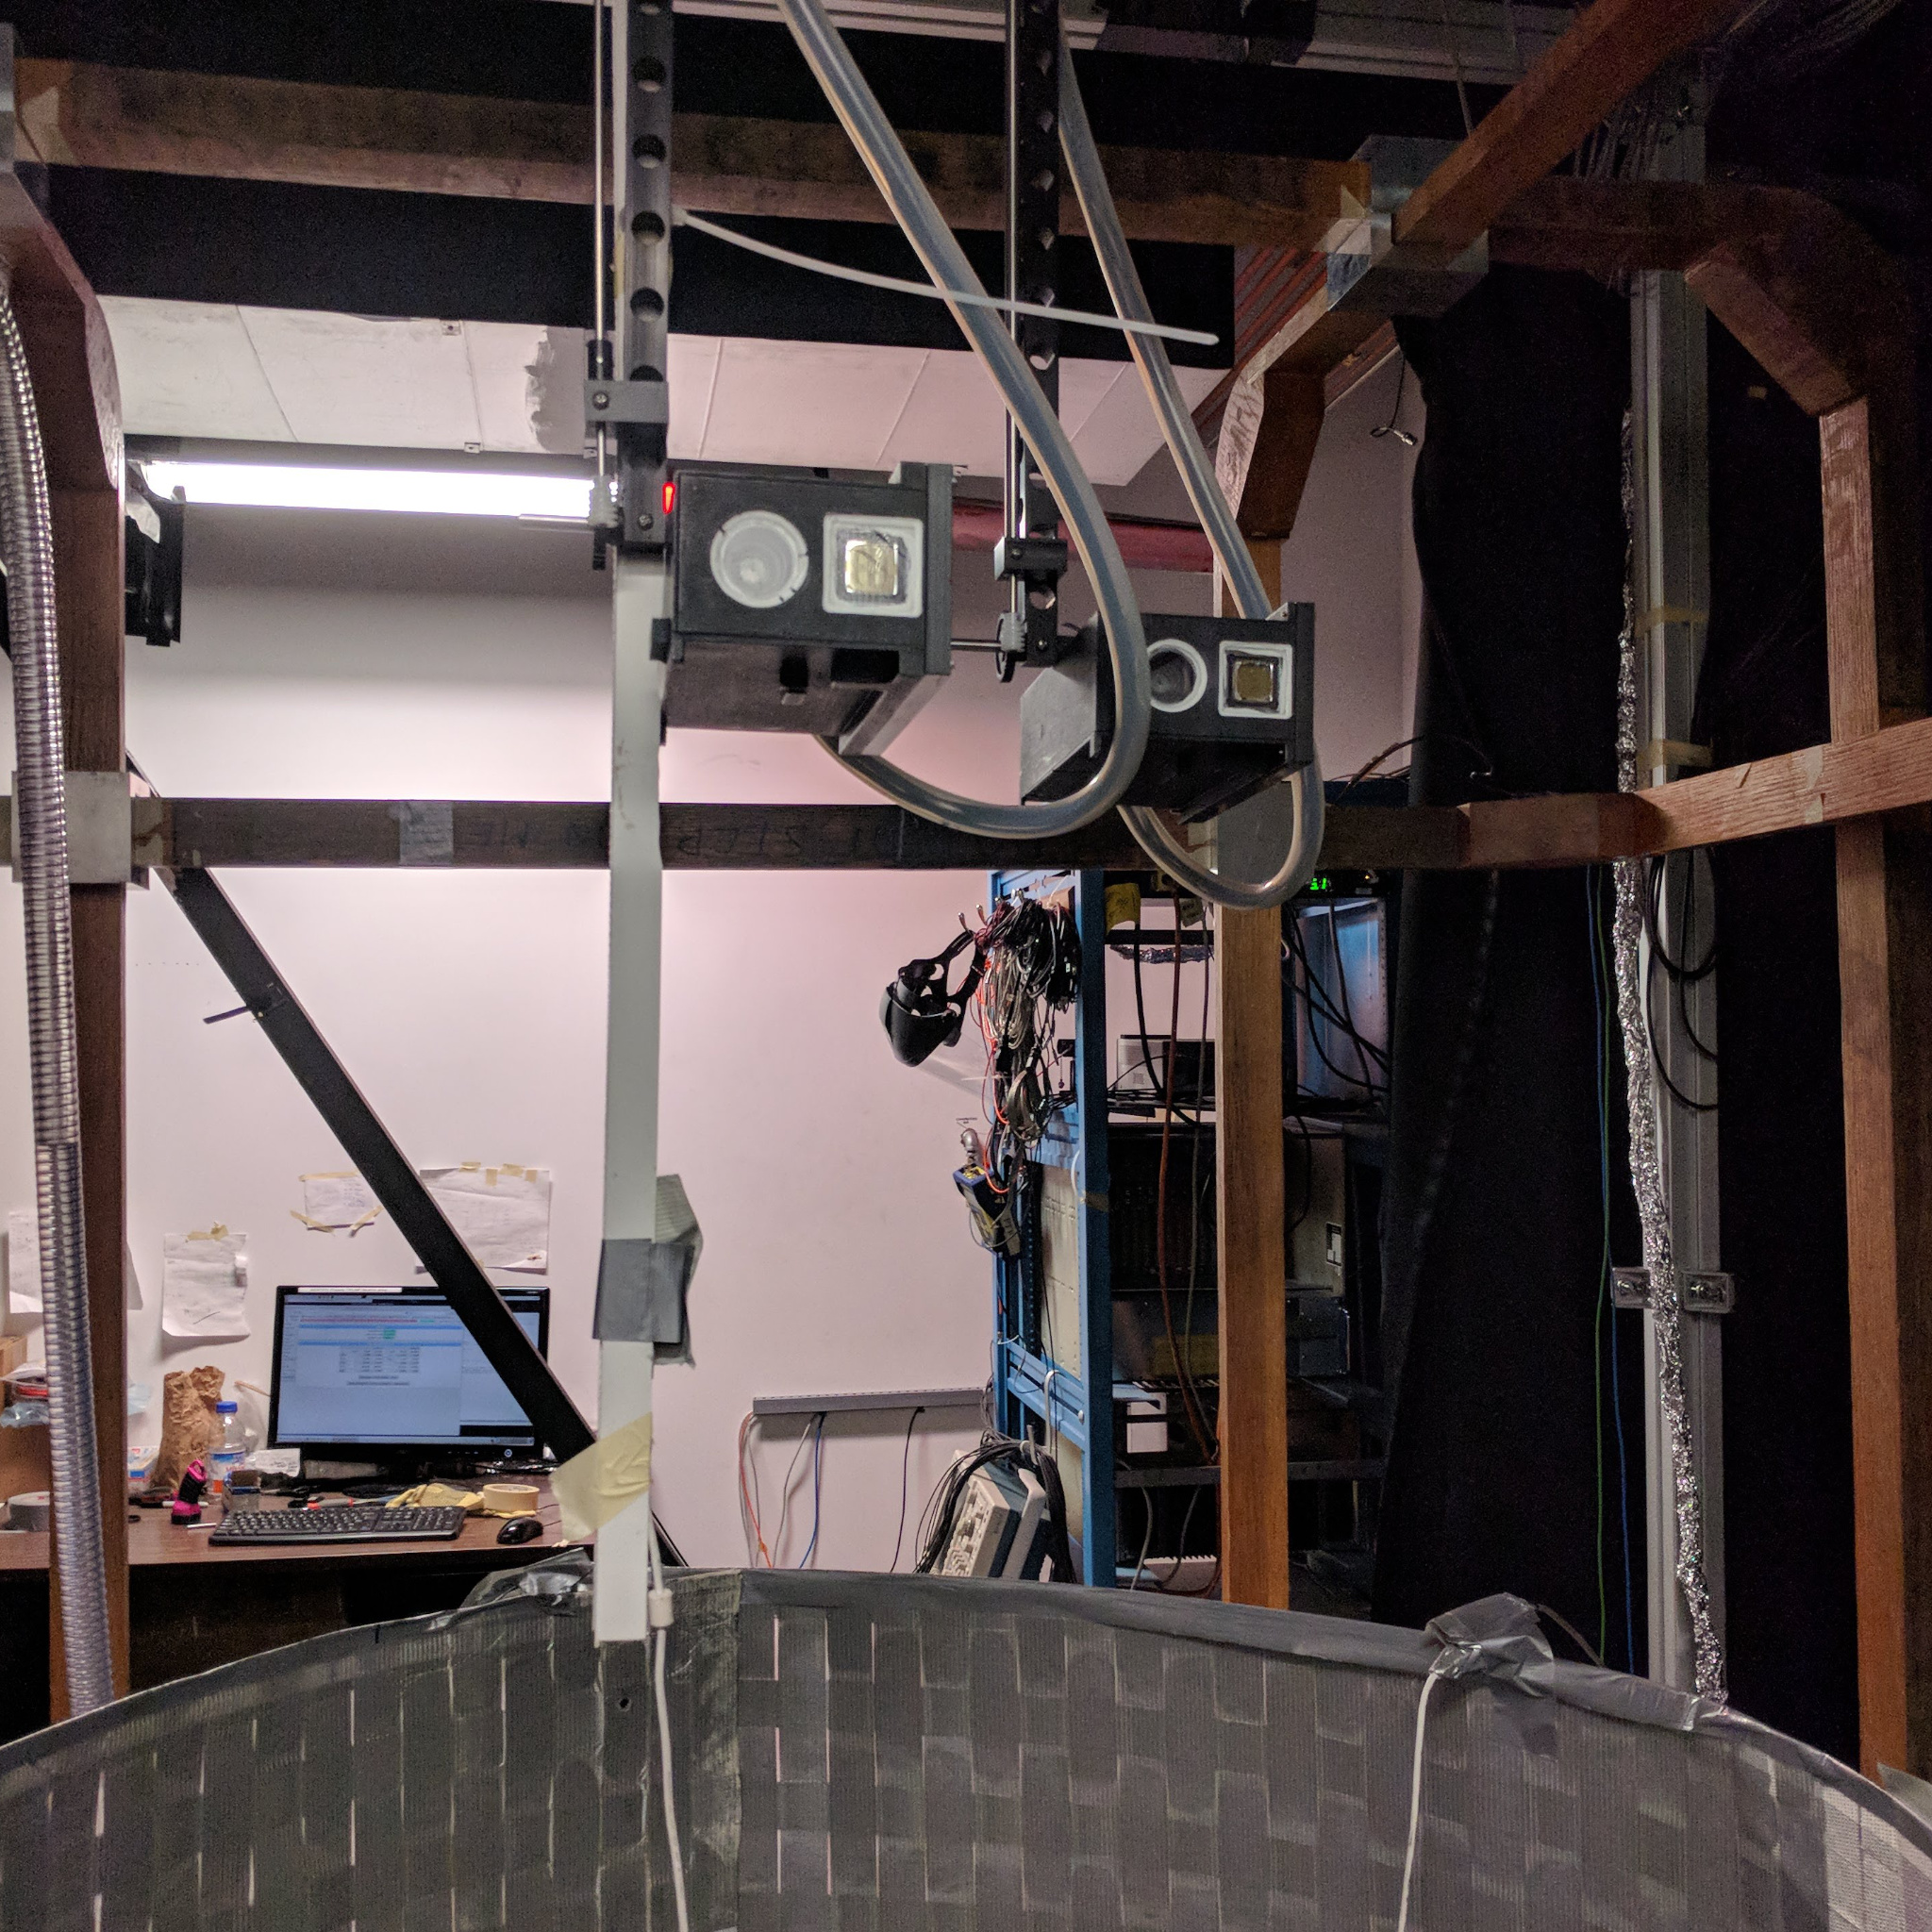
\includegraphics[width=0.325\textwidth]{images/gantriesFront.jpg}
  \caption{Gantries in position for a voltage scan. For gantry 0, this is the position $(x, y, z, \theta, \phi) = (0.3, 0.3, 0.1, -90\degree, 0\degree)$ and for gantry 1 $(0.55, 0.55, 0.1, 90\degree, 0\degree)$.\label{fig:gantryPositions}}
\end{figure}
\FloatBarrier

Then, for the two coils for that dimension, a ``voltage scan'' is run. This is a grid of voltages for the pair of coils. At each point a degauss is run to reach those voltages. An example of a voltage scan is in Figure~\ref{fig:vScan}. To run a voltage scan, there is a program stored at \texttt{\(\sim\)/scripts/optimize} which does the process above. The configuration for this is stored in \texttt{\(\sim\)/scripts/optimize.ini}. There should be four sections in this file, one for each dimension and one with some other configuration. The ``Meta'' section has one option, \texttt{steps} which controls the number of steps in the degauss.

\begin{figure}[!htb]\centering
  \resizebox{\textwidth}{!}{%% Creator: Matplotlib, PGF backend
%%
%% To include the figure in your LaTeX document, write
%%   \input{<filename>.pgf}
%%
%% Make sure the required packages are loaded in your preamble
%%   \usepackage{pgf}
%%
%% Figures using additional raster images can only be included by \input if
%% they are in the same directory as the main LaTeX file. For loading figures
%% from other directories you can use the `import` package
%%   \usepackage{import}
%% and then include the figures with
%%   \import{<path to file>}{<filename>.pgf}
%%
%% Matplotlib used the following preamble
%%   \usepackage{fontspec}
%%   \setmainfont{texgyreadventor-regular.otf}[Path=/Library/Fonts/]
%%   \setsansfont{texgyrepagella-regular.otf}[Path=/Library/Fonts/]
%%   \setmonofont{DejaVuSansMono.ttf}[Path=/usr/local/lib/python3.7/site-packages/matplotlib/mpl-data/fonts/ttf/]
%%
\begingroup%
\makeatletter%
\begin{pgfpicture}%
\pgfpathrectangle{\pgfpointorigin}{\pgfqpoint{8.000000in}{6.000000in}}%
\pgfusepath{use as bounding box, clip}%
\begin{pgfscope}%
\pgfsetbuttcap%
\pgfsetmiterjoin%
\definecolor{currentfill}{rgb}{1.000000,1.000000,1.000000}%
\pgfsetfillcolor{currentfill}%
\pgfsetlinewidth{0.000000pt}%
\definecolor{currentstroke}{rgb}{1.000000,1.000000,1.000000}%
\pgfsetstrokecolor{currentstroke}%
\pgfsetdash{}{0pt}%
\pgfpathmoveto{\pgfqpoint{0.000000in}{0.000000in}}%
\pgfpathlineto{\pgfqpoint{8.000000in}{0.000000in}}%
\pgfpathlineto{\pgfqpoint{8.000000in}{6.000000in}}%
\pgfpathlineto{\pgfqpoint{0.000000in}{6.000000in}}%
\pgfpathclose%
\pgfusepath{fill}%
\end{pgfscope}%
\begin{pgfscope}%
\pgfsetbuttcap%
\pgfsetmiterjoin%
\definecolor{currentfill}{rgb}{1.000000,1.000000,1.000000}%
\pgfsetfillcolor{currentfill}%
\pgfsetlinewidth{0.000000pt}%
\definecolor{currentstroke}{rgb}{0.000000,0.000000,0.000000}%
\pgfsetstrokecolor{currentstroke}%
\pgfsetstrokeopacity{0.000000}%
\pgfsetdash{}{0pt}%
\pgfpathmoveto{\pgfqpoint{1.340000in}{0.660000in}}%
\pgfpathlineto{\pgfqpoint{5.960000in}{0.660000in}}%
\pgfpathlineto{\pgfqpoint{5.960000in}{5.280000in}}%
\pgfpathlineto{\pgfqpoint{1.340000in}{5.280000in}}%
\pgfpathclose%
\pgfusepath{fill}%
\end{pgfscope}%
\begin{pgfscope}%
\pgfpathrectangle{\pgfqpoint{1.340000in}{0.660000in}}{\pgfqpoint{4.620000in}{4.620000in}}%
\pgfusepath{clip}%
\pgfsys@transformshift{1.340000in}{0.660000in}%
\pgftext[left,bottom]{\pgfimage[interpolate=true,width=4.625000in,height=4.625000in]{bottom-b-z-demo-img0.png}}%
\end{pgfscope}%
\begin{pgfscope}%
\pgfsetbuttcap%
\pgfsetroundjoin%
\definecolor{currentfill}{rgb}{0.000000,0.000000,0.000000}%
\pgfsetfillcolor{currentfill}%
\pgfsetlinewidth{0.803000pt}%
\definecolor{currentstroke}{rgb}{0.000000,0.000000,0.000000}%
\pgfsetstrokecolor{currentstroke}%
\pgfsetdash{}{0pt}%
\pgfsys@defobject{currentmarker}{\pgfqpoint{0.000000in}{-0.048611in}}{\pgfqpoint{0.000000in}{0.000000in}}{%
\pgfpathmoveto{\pgfqpoint{0.000000in}{0.000000in}}%
\pgfpathlineto{\pgfqpoint{0.000000in}{-0.048611in}}%
\pgfusepath{stroke,fill}%
}%
\begin{pgfscope}%
\pgfsys@transformshift{1.917500in}{0.660000in}%
\pgfsys@useobject{currentmarker}{}%
\end{pgfscope}%
\end{pgfscope}%
\begin{pgfscope}%
\definecolor{textcolor}{rgb}{0.000000,0.000000,0.000000}%
\pgfsetstrokecolor{textcolor}%
\pgfsetfillcolor{textcolor}%
\pgftext[x=1.917500in,y=0.562778in,,top]{\color{textcolor}\sffamily\fontsize{10.000000}{12.000000}\selectfont 0.5}%
\end{pgfscope}%
\begin{pgfscope}%
\pgfsetbuttcap%
\pgfsetroundjoin%
\definecolor{currentfill}{rgb}{0.000000,0.000000,0.000000}%
\pgfsetfillcolor{currentfill}%
\pgfsetlinewidth{0.803000pt}%
\definecolor{currentstroke}{rgb}{0.000000,0.000000,0.000000}%
\pgfsetstrokecolor{currentstroke}%
\pgfsetdash{}{0pt}%
\pgfsys@defobject{currentmarker}{\pgfqpoint{0.000000in}{-0.048611in}}{\pgfqpoint{0.000000in}{0.000000in}}{%
\pgfpathmoveto{\pgfqpoint{0.000000in}{0.000000in}}%
\pgfpathlineto{\pgfqpoint{0.000000in}{-0.048611in}}%
\pgfusepath{stroke,fill}%
}%
\begin{pgfscope}%
\pgfsys@transformshift{2.559167in}{0.660000in}%
\pgfsys@useobject{currentmarker}{}%
\end{pgfscope}%
\end{pgfscope}%
\begin{pgfscope}%
\definecolor{textcolor}{rgb}{0.000000,0.000000,0.000000}%
\pgfsetstrokecolor{textcolor}%
\pgfsetfillcolor{textcolor}%
\pgftext[x=2.559167in,y=0.562778in,,top]{\color{textcolor}\sffamily\fontsize{10.000000}{12.000000}\selectfont 1.0}%
\end{pgfscope}%
\begin{pgfscope}%
\pgfsetbuttcap%
\pgfsetroundjoin%
\definecolor{currentfill}{rgb}{0.000000,0.000000,0.000000}%
\pgfsetfillcolor{currentfill}%
\pgfsetlinewidth{0.803000pt}%
\definecolor{currentstroke}{rgb}{0.000000,0.000000,0.000000}%
\pgfsetstrokecolor{currentstroke}%
\pgfsetdash{}{0pt}%
\pgfsys@defobject{currentmarker}{\pgfqpoint{0.000000in}{-0.048611in}}{\pgfqpoint{0.000000in}{0.000000in}}{%
\pgfpathmoveto{\pgfqpoint{0.000000in}{0.000000in}}%
\pgfpathlineto{\pgfqpoint{0.000000in}{-0.048611in}}%
\pgfusepath{stroke,fill}%
}%
\begin{pgfscope}%
\pgfsys@transformshift{3.200833in}{0.660000in}%
\pgfsys@useobject{currentmarker}{}%
\end{pgfscope}%
\end{pgfscope}%
\begin{pgfscope}%
\definecolor{textcolor}{rgb}{0.000000,0.000000,0.000000}%
\pgfsetstrokecolor{textcolor}%
\pgfsetfillcolor{textcolor}%
\pgftext[x=3.200833in,y=0.562778in,,top]{\color{textcolor}\sffamily\fontsize{10.000000}{12.000000}\selectfont 1.5}%
\end{pgfscope}%
\begin{pgfscope}%
\pgfsetbuttcap%
\pgfsetroundjoin%
\definecolor{currentfill}{rgb}{0.000000,0.000000,0.000000}%
\pgfsetfillcolor{currentfill}%
\pgfsetlinewidth{0.803000pt}%
\definecolor{currentstroke}{rgb}{0.000000,0.000000,0.000000}%
\pgfsetstrokecolor{currentstroke}%
\pgfsetdash{}{0pt}%
\pgfsys@defobject{currentmarker}{\pgfqpoint{0.000000in}{-0.048611in}}{\pgfqpoint{0.000000in}{0.000000in}}{%
\pgfpathmoveto{\pgfqpoint{0.000000in}{0.000000in}}%
\pgfpathlineto{\pgfqpoint{0.000000in}{-0.048611in}}%
\pgfusepath{stroke,fill}%
}%
\begin{pgfscope}%
\pgfsys@transformshift{3.842500in}{0.660000in}%
\pgfsys@useobject{currentmarker}{}%
\end{pgfscope}%
\end{pgfscope}%
\begin{pgfscope}%
\definecolor{textcolor}{rgb}{0.000000,0.000000,0.000000}%
\pgfsetstrokecolor{textcolor}%
\pgfsetfillcolor{textcolor}%
\pgftext[x=3.842500in,y=0.562778in,,top]{\color{textcolor}\sffamily\fontsize{10.000000}{12.000000}\selectfont 2.0}%
\end{pgfscope}%
\begin{pgfscope}%
\pgfsetbuttcap%
\pgfsetroundjoin%
\definecolor{currentfill}{rgb}{0.000000,0.000000,0.000000}%
\pgfsetfillcolor{currentfill}%
\pgfsetlinewidth{0.803000pt}%
\definecolor{currentstroke}{rgb}{0.000000,0.000000,0.000000}%
\pgfsetstrokecolor{currentstroke}%
\pgfsetdash{}{0pt}%
\pgfsys@defobject{currentmarker}{\pgfqpoint{0.000000in}{-0.048611in}}{\pgfqpoint{0.000000in}{0.000000in}}{%
\pgfpathmoveto{\pgfqpoint{0.000000in}{0.000000in}}%
\pgfpathlineto{\pgfqpoint{0.000000in}{-0.048611in}}%
\pgfusepath{stroke,fill}%
}%
\begin{pgfscope}%
\pgfsys@transformshift{4.484167in}{0.660000in}%
\pgfsys@useobject{currentmarker}{}%
\end{pgfscope}%
\end{pgfscope}%
\begin{pgfscope}%
\definecolor{textcolor}{rgb}{0.000000,0.000000,0.000000}%
\pgfsetstrokecolor{textcolor}%
\pgfsetfillcolor{textcolor}%
\pgftext[x=4.484167in,y=0.562778in,,top]{\color{textcolor}\sffamily\fontsize{10.000000}{12.000000}\selectfont 2.5}%
\end{pgfscope}%
\begin{pgfscope}%
\pgfsetbuttcap%
\pgfsetroundjoin%
\definecolor{currentfill}{rgb}{0.000000,0.000000,0.000000}%
\pgfsetfillcolor{currentfill}%
\pgfsetlinewidth{0.803000pt}%
\definecolor{currentstroke}{rgb}{0.000000,0.000000,0.000000}%
\pgfsetstrokecolor{currentstroke}%
\pgfsetdash{}{0pt}%
\pgfsys@defobject{currentmarker}{\pgfqpoint{0.000000in}{-0.048611in}}{\pgfqpoint{0.000000in}{0.000000in}}{%
\pgfpathmoveto{\pgfqpoint{0.000000in}{0.000000in}}%
\pgfpathlineto{\pgfqpoint{0.000000in}{-0.048611in}}%
\pgfusepath{stroke,fill}%
}%
\begin{pgfscope}%
\pgfsys@transformshift{5.125833in}{0.660000in}%
\pgfsys@useobject{currentmarker}{}%
\end{pgfscope}%
\end{pgfscope}%
\begin{pgfscope}%
\definecolor{textcolor}{rgb}{0.000000,0.000000,0.000000}%
\pgfsetstrokecolor{textcolor}%
\pgfsetfillcolor{textcolor}%
\pgftext[x=5.125833in,y=0.562778in,,top]{\color{textcolor}\sffamily\fontsize{10.000000}{12.000000}\selectfont 3.0}%
\end{pgfscope}%
\begin{pgfscope}%
\pgfsetbuttcap%
\pgfsetroundjoin%
\definecolor{currentfill}{rgb}{0.000000,0.000000,0.000000}%
\pgfsetfillcolor{currentfill}%
\pgfsetlinewidth{0.803000pt}%
\definecolor{currentstroke}{rgb}{0.000000,0.000000,0.000000}%
\pgfsetstrokecolor{currentstroke}%
\pgfsetdash{}{0pt}%
\pgfsys@defobject{currentmarker}{\pgfqpoint{0.000000in}{-0.048611in}}{\pgfqpoint{0.000000in}{0.000000in}}{%
\pgfpathmoveto{\pgfqpoint{0.000000in}{0.000000in}}%
\pgfpathlineto{\pgfqpoint{0.000000in}{-0.048611in}}%
\pgfusepath{stroke,fill}%
}%
\begin{pgfscope}%
\pgfsys@transformshift{5.767500in}{0.660000in}%
\pgfsys@useobject{currentmarker}{}%
\end{pgfscope}%
\end{pgfscope}%
\begin{pgfscope}%
\definecolor{textcolor}{rgb}{0.000000,0.000000,0.000000}%
\pgfsetstrokecolor{textcolor}%
\pgfsetfillcolor{textcolor}%
\pgftext[x=5.767500in,y=0.562778in,,top]{\color{textcolor}\sffamily\fontsize{10.000000}{12.000000}\selectfont 3.5}%
\end{pgfscope}%
\begin{pgfscope}%
\definecolor{textcolor}{rgb}{0.000000,0.000000,0.000000}%
\pgfsetstrokecolor{textcolor}%
\pgfsetfillcolor{textcolor}%
\pgftext[x=3.650000in,y=0.367361in,,top]{\color{textcolor}\sffamily\fontsize{10.000000}{12.000000}\selectfont Voltage for Coil 1 [V]}%
\end{pgfscope}%
\begin{pgfscope}%
\pgfsetbuttcap%
\pgfsetroundjoin%
\definecolor{currentfill}{rgb}{0.000000,0.000000,0.000000}%
\pgfsetfillcolor{currentfill}%
\pgfsetlinewidth{0.803000pt}%
\definecolor{currentstroke}{rgb}{0.000000,0.000000,0.000000}%
\pgfsetstrokecolor{currentstroke}%
\pgfsetdash{}{0pt}%
\pgfsys@defobject{currentmarker}{\pgfqpoint{-0.048611in}{0.000000in}}{\pgfqpoint{0.000000in}{0.000000in}}{%
\pgfpathmoveto{\pgfqpoint{0.000000in}{0.000000in}}%
\pgfpathlineto{\pgfqpoint{-0.048611in}{0.000000in}}%
\pgfusepath{stroke,fill}%
}%
\begin{pgfscope}%
\pgfsys@transformshift{1.340000in}{1.237500in}%
\pgfsys@useobject{currentmarker}{}%
\end{pgfscope}%
\end{pgfscope}%
\begin{pgfscope}%
\definecolor{textcolor}{rgb}{0.000000,0.000000,0.000000}%
\pgfsetstrokecolor{textcolor}%
\pgfsetfillcolor{textcolor}%
\pgftext[x=1.069167in,y=1.187083in,left,base]{\color{textcolor}\sffamily\fontsize{10.000000}{12.000000}\selectfont 0.5}%
\end{pgfscope}%
\begin{pgfscope}%
\pgfsetbuttcap%
\pgfsetroundjoin%
\definecolor{currentfill}{rgb}{0.000000,0.000000,0.000000}%
\pgfsetfillcolor{currentfill}%
\pgfsetlinewidth{0.803000pt}%
\definecolor{currentstroke}{rgb}{0.000000,0.000000,0.000000}%
\pgfsetstrokecolor{currentstroke}%
\pgfsetdash{}{0pt}%
\pgfsys@defobject{currentmarker}{\pgfqpoint{-0.048611in}{0.000000in}}{\pgfqpoint{0.000000in}{0.000000in}}{%
\pgfpathmoveto{\pgfqpoint{0.000000in}{0.000000in}}%
\pgfpathlineto{\pgfqpoint{-0.048611in}{0.000000in}}%
\pgfusepath{stroke,fill}%
}%
\begin{pgfscope}%
\pgfsys@transformshift{1.340000in}{1.879167in}%
\pgfsys@useobject{currentmarker}{}%
\end{pgfscope}%
\end{pgfscope}%
\begin{pgfscope}%
\definecolor{textcolor}{rgb}{0.000000,0.000000,0.000000}%
\pgfsetstrokecolor{textcolor}%
\pgfsetfillcolor{textcolor}%
\pgftext[x=1.069167in,y=1.828750in,left,base]{\color{textcolor}\sffamily\fontsize{10.000000}{12.000000}\selectfont 1.0}%
\end{pgfscope}%
\begin{pgfscope}%
\pgfsetbuttcap%
\pgfsetroundjoin%
\definecolor{currentfill}{rgb}{0.000000,0.000000,0.000000}%
\pgfsetfillcolor{currentfill}%
\pgfsetlinewidth{0.803000pt}%
\definecolor{currentstroke}{rgb}{0.000000,0.000000,0.000000}%
\pgfsetstrokecolor{currentstroke}%
\pgfsetdash{}{0pt}%
\pgfsys@defobject{currentmarker}{\pgfqpoint{-0.048611in}{0.000000in}}{\pgfqpoint{0.000000in}{0.000000in}}{%
\pgfpathmoveto{\pgfqpoint{0.000000in}{0.000000in}}%
\pgfpathlineto{\pgfqpoint{-0.048611in}{0.000000in}}%
\pgfusepath{stroke,fill}%
}%
\begin{pgfscope}%
\pgfsys@transformshift{1.340000in}{2.520833in}%
\pgfsys@useobject{currentmarker}{}%
\end{pgfscope}%
\end{pgfscope}%
\begin{pgfscope}%
\definecolor{textcolor}{rgb}{0.000000,0.000000,0.000000}%
\pgfsetstrokecolor{textcolor}%
\pgfsetfillcolor{textcolor}%
\pgftext[x=1.069167in,y=2.470417in,left,base]{\color{textcolor}\sffamily\fontsize{10.000000}{12.000000}\selectfont 1.5}%
\end{pgfscope}%
\begin{pgfscope}%
\pgfsetbuttcap%
\pgfsetroundjoin%
\definecolor{currentfill}{rgb}{0.000000,0.000000,0.000000}%
\pgfsetfillcolor{currentfill}%
\pgfsetlinewidth{0.803000pt}%
\definecolor{currentstroke}{rgb}{0.000000,0.000000,0.000000}%
\pgfsetstrokecolor{currentstroke}%
\pgfsetdash{}{0pt}%
\pgfsys@defobject{currentmarker}{\pgfqpoint{-0.048611in}{0.000000in}}{\pgfqpoint{0.000000in}{0.000000in}}{%
\pgfpathmoveto{\pgfqpoint{0.000000in}{0.000000in}}%
\pgfpathlineto{\pgfqpoint{-0.048611in}{0.000000in}}%
\pgfusepath{stroke,fill}%
}%
\begin{pgfscope}%
\pgfsys@transformshift{1.340000in}{3.162500in}%
\pgfsys@useobject{currentmarker}{}%
\end{pgfscope}%
\end{pgfscope}%
\begin{pgfscope}%
\definecolor{textcolor}{rgb}{0.000000,0.000000,0.000000}%
\pgfsetstrokecolor{textcolor}%
\pgfsetfillcolor{textcolor}%
\pgftext[x=1.069167in,y=3.112083in,left,base]{\color{textcolor}\sffamily\fontsize{10.000000}{12.000000}\selectfont 2.0}%
\end{pgfscope}%
\begin{pgfscope}%
\pgfsetbuttcap%
\pgfsetroundjoin%
\definecolor{currentfill}{rgb}{0.000000,0.000000,0.000000}%
\pgfsetfillcolor{currentfill}%
\pgfsetlinewidth{0.803000pt}%
\definecolor{currentstroke}{rgb}{0.000000,0.000000,0.000000}%
\pgfsetstrokecolor{currentstroke}%
\pgfsetdash{}{0pt}%
\pgfsys@defobject{currentmarker}{\pgfqpoint{-0.048611in}{0.000000in}}{\pgfqpoint{0.000000in}{0.000000in}}{%
\pgfpathmoveto{\pgfqpoint{0.000000in}{0.000000in}}%
\pgfpathlineto{\pgfqpoint{-0.048611in}{0.000000in}}%
\pgfusepath{stroke,fill}%
}%
\begin{pgfscope}%
\pgfsys@transformshift{1.340000in}{3.804167in}%
\pgfsys@useobject{currentmarker}{}%
\end{pgfscope}%
\end{pgfscope}%
\begin{pgfscope}%
\definecolor{textcolor}{rgb}{0.000000,0.000000,0.000000}%
\pgfsetstrokecolor{textcolor}%
\pgfsetfillcolor{textcolor}%
\pgftext[x=1.069167in,y=3.753750in,left,base]{\color{textcolor}\sffamily\fontsize{10.000000}{12.000000}\selectfont 2.5}%
\end{pgfscope}%
\begin{pgfscope}%
\pgfsetbuttcap%
\pgfsetroundjoin%
\definecolor{currentfill}{rgb}{0.000000,0.000000,0.000000}%
\pgfsetfillcolor{currentfill}%
\pgfsetlinewidth{0.803000pt}%
\definecolor{currentstroke}{rgb}{0.000000,0.000000,0.000000}%
\pgfsetstrokecolor{currentstroke}%
\pgfsetdash{}{0pt}%
\pgfsys@defobject{currentmarker}{\pgfqpoint{-0.048611in}{0.000000in}}{\pgfqpoint{0.000000in}{0.000000in}}{%
\pgfpathmoveto{\pgfqpoint{0.000000in}{0.000000in}}%
\pgfpathlineto{\pgfqpoint{-0.048611in}{0.000000in}}%
\pgfusepath{stroke,fill}%
}%
\begin{pgfscope}%
\pgfsys@transformshift{1.340000in}{4.445833in}%
\pgfsys@useobject{currentmarker}{}%
\end{pgfscope}%
\end{pgfscope}%
\begin{pgfscope}%
\definecolor{textcolor}{rgb}{0.000000,0.000000,0.000000}%
\pgfsetstrokecolor{textcolor}%
\pgfsetfillcolor{textcolor}%
\pgftext[x=1.069167in,y=4.395417in,left,base]{\color{textcolor}\sffamily\fontsize{10.000000}{12.000000}\selectfont 3.0}%
\end{pgfscope}%
\begin{pgfscope}%
\pgfsetbuttcap%
\pgfsetroundjoin%
\definecolor{currentfill}{rgb}{0.000000,0.000000,0.000000}%
\pgfsetfillcolor{currentfill}%
\pgfsetlinewidth{0.803000pt}%
\definecolor{currentstroke}{rgb}{0.000000,0.000000,0.000000}%
\pgfsetstrokecolor{currentstroke}%
\pgfsetdash{}{0pt}%
\pgfsys@defobject{currentmarker}{\pgfqpoint{-0.048611in}{0.000000in}}{\pgfqpoint{0.000000in}{0.000000in}}{%
\pgfpathmoveto{\pgfqpoint{0.000000in}{0.000000in}}%
\pgfpathlineto{\pgfqpoint{-0.048611in}{0.000000in}}%
\pgfusepath{stroke,fill}%
}%
\begin{pgfscope}%
\pgfsys@transformshift{1.340000in}{5.087500in}%
\pgfsys@useobject{currentmarker}{}%
\end{pgfscope}%
\end{pgfscope}%
\begin{pgfscope}%
\definecolor{textcolor}{rgb}{0.000000,0.000000,0.000000}%
\pgfsetstrokecolor{textcolor}%
\pgfsetfillcolor{textcolor}%
\pgftext[x=1.069167in,y=5.037083in,left,base]{\color{textcolor}\sffamily\fontsize{10.000000}{12.000000}\selectfont 3.5}%
\end{pgfscope}%
\begin{pgfscope}%
\definecolor{textcolor}{rgb}{0.000000,0.000000,0.000000}%
\pgfsetstrokecolor{textcolor}%
\pgfsetfillcolor{textcolor}%
\pgftext[x=1.013611in,y=2.970000in,,bottom,rotate=90.000000]{\color{textcolor}\sffamily\fontsize{10.000000}{12.000000}\selectfont Voltage for Coil 2 [V]}%
\end{pgfscope}%
\begin{pgfscope}%
\pgfsetrectcap%
\pgfsetmiterjoin%
\pgfsetlinewidth{0.803000pt}%
\definecolor{currentstroke}{rgb}{0.000000,0.000000,0.000000}%
\pgfsetstrokecolor{currentstroke}%
\pgfsetdash{}{0pt}%
\pgfpathmoveto{\pgfqpoint{1.340000in}{0.660000in}}%
\pgfpathlineto{\pgfqpoint{1.340000in}{5.280000in}}%
\pgfusepath{stroke}%
\end{pgfscope}%
\begin{pgfscope}%
\pgfsetrectcap%
\pgfsetmiterjoin%
\pgfsetlinewidth{0.803000pt}%
\definecolor{currentstroke}{rgb}{0.000000,0.000000,0.000000}%
\pgfsetstrokecolor{currentstroke}%
\pgfsetdash{}{0pt}%
\pgfpathmoveto{\pgfqpoint{5.960000in}{0.660000in}}%
\pgfpathlineto{\pgfqpoint{5.960000in}{5.280000in}}%
\pgfusepath{stroke}%
\end{pgfscope}%
\begin{pgfscope}%
\pgfsetrectcap%
\pgfsetmiterjoin%
\pgfsetlinewidth{0.803000pt}%
\definecolor{currentstroke}{rgb}{0.000000,0.000000,0.000000}%
\pgfsetstrokecolor{currentstroke}%
\pgfsetdash{}{0pt}%
\pgfpathmoveto{\pgfqpoint{1.340000in}{0.660000in}}%
\pgfpathlineto{\pgfqpoint{5.960000in}{0.660000in}}%
\pgfusepath{stroke}%
\end{pgfscope}%
\begin{pgfscope}%
\pgfsetrectcap%
\pgfsetmiterjoin%
\pgfsetlinewidth{0.803000pt}%
\definecolor{currentstroke}{rgb}{0.000000,0.000000,0.000000}%
\pgfsetstrokecolor{currentstroke}%
\pgfsetdash{}{0pt}%
\pgfpathmoveto{\pgfqpoint{1.340000in}{5.280000in}}%
\pgfpathlineto{\pgfqpoint{5.960000in}{5.280000in}}%
\pgfusepath{stroke}%
\end{pgfscope}%
\begin{pgfscope}%
\definecolor{textcolor}{rgb}{0.000000,0.000000,0.000000}%
\pgfsetstrokecolor{textcolor}%
\pgfsetfillcolor{textcolor}%
\pgftext[x=3.650000in,y=5.363333in,,base]{\color{textcolor}\sffamily\fontsize{12.000000}{14.400000}\selectfont Bottom \(\displaystyle B_z\) [G]}%
\end{pgfscope}%
\begin{pgfscope}%
\pgfpathrectangle{\pgfqpoint{6.270000in}{0.660000in}}{\pgfqpoint{0.231000in}{4.620000in}}%
\pgfusepath{clip}%
\pgfsetbuttcap%
\pgfsetmiterjoin%
\definecolor{currentfill}{rgb}{1.000000,1.000000,1.000000}%
\pgfsetfillcolor{currentfill}%
\pgfsetlinewidth{0.010037pt}%
\definecolor{currentstroke}{rgb}{1.000000,1.000000,1.000000}%
\pgfsetstrokecolor{currentstroke}%
\pgfsetdash{}{0pt}%
\pgfpathmoveto{\pgfqpoint{6.270000in}{0.660000in}}%
\pgfpathlineto{\pgfqpoint{6.270000in}{0.678047in}}%
\pgfpathlineto{\pgfqpoint{6.270000in}{5.261953in}}%
\pgfpathlineto{\pgfqpoint{6.270000in}{5.280000in}}%
\pgfpathlineto{\pgfqpoint{6.501000in}{5.280000in}}%
\pgfpathlineto{\pgfqpoint{6.501000in}{5.261953in}}%
\pgfpathlineto{\pgfqpoint{6.501000in}{0.678047in}}%
\pgfpathlineto{\pgfqpoint{6.501000in}{0.660000in}}%
\pgfpathclose%
\pgfusepath{stroke,fill}%
\end{pgfscope}%
\begin{pgfscope}%
\pgfsys@transformshift{6.270833in}{0.661458in}%
\pgftext[left,bottom]{\pgfimage[interpolate=true,width=0.229167in,height=4.619792in]{bottom-b-z-demo-img1.png}}%
\end{pgfscope}%
\begin{pgfscope}%
\pgfsetbuttcap%
\pgfsetroundjoin%
\definecolor{currentfill}{rgb}{0.000000,0.000000,0.000000}%
\pgfsetfillcolor{currentfill}%
\pgfsetlinewidth{0.803000pt}%
\definecolor{currentstroke}{rgb}{0.000000,0.000000,0.000000}%
\pgfsetstrokecolor{currentstroke}%
\pgfsetdash{}{0pt}%
\pgfsys@defobject{currentmarker}{\pgfqpoint{0.000000in}{0.000000in}}{\pgfqpoint{0.048611in}{0.000000in}}{%
\pgfpathmoveto{\pgfqpoint{0.000000in}{0.000000in}}%
\pgfpathlineto{\pgfqpoint{0.048611in}{0.000000in}}%
\pgfusepath{stroke,fill}%
}%
\begin{pgfscope}%
\pgfsys@transformshift{6.501000in}{0.979021in}%
\pgfsys@useobject{currentmarker}{}%
\end{pgfscope}%
\end{pgfscope}%
\begin{pgfscope}%
\definecolor{textcolor}{rgb}{0.000000,0.000000,0.000000}%
\pgfsetstrokecolor{textcolor}%
\pgfsetfillcolor{textcolor}%
\pgftext[x=6.598222in,y=0.928605in,left,base]{\color{textcolor}\sffamily\fontsize{10.000000}{12.000000}\selectfont −0.3}%
\end{pgfscope}%
\begin{pgfscope}%
\pgfsetbuttcap%
\pgfsetroundjoin%
\definecolor{currentfill}{rgb}{0.000000,0.000000,0.000000}%
\pgfsetfillcolor{currentfill}%
\pgfsetlinewidth{0.803000pt}%
\definecolor{currentstroke}{rgb}{0.000000,0.000000,0.000000}%
\pgfsetstrokecolor{currentstroke}%
\pgfsetdash{}{0pt}%
\pgfsys@defobject{currentmarker}{\pgfqpoint{0.000000in}{0.000000in}}{\pgfqpoint{0.048611in}{0.000000in}}{%
\pgfpathmoveto{\pgfqpoint{0.000000in}{0.000000in}}%
\pgfpathlineto{\pgfqpoint{0.048611in}{0.000000in}}%
\pgfusepath{stroke,fill}%
}%
\begin{pgfscope}%
\pgfsys@transformshift{6.501000in}{1.642681in}%
\pgfsys@useobject{currentmarker}{}%
\end{pgfscope}%
\end{pgfscope}%
\begin{pgfscope}%
\definecolor{textcolor}{rgb}{0.000000,0.000000,0.000000}%
\pgfsetstrokecolor{textcolor}%
\pgfsetfillcolor{textcolor}%
\pgftext[x=6.598222in,y=1.592264in,left,base]{\color{textcolor}\sffamily\fontsize{10.000000}{12.000000}\selectfont −0.2}%
\end{pgfscope}%
\begin{pgfscope}%
\pgfsetbuttcap%
\pgfsetroundjoin%
\definecolor{currentfill}{rgb}{0.000000,0.000000,0.000000}%
\pgfsetfillcolor{currentfill}%
\pgfsetlinewidth{0.803000pt}%
\definecolor{currentstroke}{rgb}{0.000000,0.000000,0.000000}%
\pgfsetstrokecolor{currentstroke}%
\pgfsetdash{}{0pt}%
\pgfsys@defobject{currentmarker}{\pgfqpoint{0.000000in}{0.000000in}}{\pgfqpoint{0.048611in}{0.000000in}}{%
\pgfpathmoveto{\pgfqpoint{0.000000in}{0.000000in}}%
\pgfpathlineto{\pgfqpoint{0.048611in}{0.000000in}}%
\pgfusepath{stroke,fill}%
}%
\begin{pgfscope}%
\pgfsys@transformshift{6.501000in}{2.306340in}%
\pgfsys@useobject{currentmarker}{}%
\end{pgfscope}%
\end{pgfscope}%
\begin{pgfscope}%
\definecolor{textcolor}{rgb}{0.000000,0.000000,0.000000}%
\pgfsetstrokecolor{textcolor}%
\pgfsetfillcolor{textcolor}%
\pgftext[x=6.598222in,y=2.255924in,left,base]{\color{textcolor}\sffamily\fontsize{10.000000}{12.000000}\selectfont −0.1}%
\end{pgfscope}%
\begin{pgfscope}%
\pgfsetbuttcap%
\pgfsetroundjoin%
\definecolor{currentfill}{rgb}{0.000000,0.000000,0.000000}%
\pgfsetfillcolor{currentfill}%
\pgfsetlinewidth{0.803000pt}%
\definecolor{currentstroke}{rgb}{0.000000,0.000000,0.000000}%
\pgfsetstrokecolor{currentstroke}%
\pgfsetdash{}{0pt}%
\pgfsys@defobject{currentmarker}{\pgfqpoint{0.000000in}{0.000000in}}{\pgfqpoint{0.048611in}{0.000000in}}{%
\pgfpathmoveto{\pgfqpoint{0.000000in}{0.000000in}}%
\pgfpathlineto{\pgfqpoint{0.048611in}{0.000000in}}%
\pgfusepath{stroke,fill}%
}%
\begin{pgfscope}%
\pgfsys@transformshift{6.501000in}{2.970000in}%
\pgfsys@useobject{currentmarker}{}%
\end{pgfscope}%
\end{pgfscope}%
\begin{pgfscope}%
\definecolor{textcolor}{rgb}{0.000000,0.000000,0.000000}%
\pgfsetstrokecolor{textcolor}%
\pgfsetfillcolor{textcolor}%
\pgftext[x=6.598222in,y=2.919583in,left,base]{\color{textcolor}\sffamily\fontsize{10.000000}{12.000000}\selectfont 0.0}%
\end{pgfscope}%
\begin{pgfscope}%
\pgfsetbuttcap%
\pgfsetroundjoin%
\definecolor{currentfill}{rgb}{0.000000,0.000000,0.000000}%
\pgfsetfillcolor{currentfill}%
\pgfsetlinewidth{0.803000pt}%
\definecolor{currentstroke}{rgb}{0.000000,0.000000,0.000000}%
\pgfsetstrokecolor{currentstroke}%
\pgfsetdash{}{0pt}%
\pgfsys@defobject{currentmarker}{\pgfqpoint{0.000000in}{0.000000in}}{\pgfqpoint{0.048611in}{0.000000in}}{%
\pgfpathmoveto{\pgfqpoint{0.000000in}{0.000000in}}%
\pgfpathlineto{\pgfqpoint{0.048611in}{0.000000in}}%
\pgfusepath{stroke,fill}%
}%
\begin{pgfscope}%
\pgfsys@transformshift{6.501000in}{3.633660in}%
\pgfsys@useobject{currentmarker}{}%
\end{pgfscope}%
\end{pgfscope}%
\begin{pgfscope}%
\definecolor{textcolor}{rgb}{0.000000,0.000000,0.000000}%
\pgfsetstrokecolor{textcolor}%
\pgfsetfillcolor{textcolor}%
\pgftext[x=6.598222in,y=3.583243in,left,base]{\color{textcolor}\sffamily\fontsize{10.000000}{12.000000}\selectfont 0.1}%
\end{pgfscope}%
\begin{pgfscope}%
\pgfsetbuttcap%
\pgfsetroundjoin%
\definecolor{currentfill}{rgb}{0.000000,0.000000,0.000000}%
\pgfsetfillcolor{currentfill}%
\pgfsetlinewidth{0.803000pt}%
\definecolor{currentstroke}{rgb}{0.000000,0.000000,0.000000}%
\pgfsetstrokecolor{currentstroke}%
\pgfsetdash{}{0pt}%
\pgfsys@defobject{currentmarker}{\pgfqpoint{0.000000in}{0.000000in}}{\pgfqpoint{0.048611in}{0.000000in}}{%
\pgfpathmoveto{\pgfqpoint{0.000000in}{0.000000in}}%
\pgfpathlineto{\pgfqpoint{0.048611in}{0.000000in}}%
\pgfusepath{stroke,fill}%
}%
\begin{pgfscope}%
\pgfsys@transformshift{6.501000in}{4.297319in}%
\pgfsys@useobject{currentmarker}{}%
\end{pgfscope}%
\end{pgfscope}%
\begin{pgfscope}%
\definecolor{textcolor}{rgb}{0.000000,0.000000,0.000000}%
\pgfsetstrokecolor{textcolor}%
\pgfsetfillcolor{textcolor}%
\pgftext[x=6.598222in,y=4.246903in,left,base]{\color{textcolor}\sffamily\fontsize{10.000000}{12.000000}\selectfont 0.2}%
\end{pgfscope}%
\begin{pgfscope}%
\pgfsetbuttcap%
\pgfsetroundjoin%
\definecolor{currentfill}{rgb}{0.000000,0.000000,0.000000}%
\pgfsetfillcolor{currentfill}%
\pgfsetlinewidth{0.803000pt}%
\definecolor{currentstroke}{rgb}{0.000000,0.000000,0.000000}%
\pgfsetstrokecolor{currentstroke}%
\pgfsetdash{}{0pt}%
\pgfsys@defobject{currentmarker}{\pgfqpoint{0.000000in}{0.000000in}}{\pgfqpoint{0.048611in}{0.000000in}}{%
\pgfpathmoveto{\pgfqpoint{0.000000in}{0.000000in}}%
\pgfpathlineto{\pgfqpoint{0.048611in}{0.000000in}}%
\pgfusepath{stroke,fill}%
}%
\begin{pgfscope}%
\pgfsys@transformshift{6.501000in}{4.960979in}%
\pgfsys@useobject{currentmarker}{}%
\end{pgfscope}%
\end{pgfscope}%
\begin{pgfscope}%
\definecolor{textcolor}{rgb}{0.000000,0.000000,0.000000}%
\pgfsetstrokecolor{textcolor}%
\pgfsetfillcolor{textcolor}%
\pgftext[x=6.598222in,y=4.910562in,left,base]{\color{textcolor}\sffamily\fontsize{10.000000}{12.000000}\selectfont 0.3}%
\end{pgfscope}%
\begin{pgfscope}%
\pgfsetbuttcap%
\pgfsetmiterjoin%
\pgfsetlinewidth{0.803000pt}%
\definecolor{currentstroke}{rgb}{0.000000,0.000000,0.000000}%
\pgfsetstrokecolor{currentstroke}%
\pgfsetdash{}{0pt}%
\pgfpathmoveto{\pgfqpoint{6.270000in}{0.660000in}}%
\pgfpathlineto{\pgfqpoint{6.270000in}{0.678047in}}%
\pgfpathlineto{\pgfqpoint{6.270000in}{5.261953in}}%
\pgfpathlineto{\pgfqpoint{6.270000in}{5.280000in}}%
\pgfpathlineto{\pgfqpoint{6.501000in}{5.280000in}}%
\pgfpathlineto{\pgfqpoint{6.501000in}{5.261953in}}%
\pgfpathlineto{\pgfqpoint{6.501000in}{0.678047in}}%
\pgfpathlineto{\pgfqpoint{6.501000in}{0.660000in}}%
\pgfpathclose%
\pgfusepath{stroke}%
\end{pgfscope}%
\end{pgfpicture}%
\makeatother%
\endgroup%
}
  \caption{An example of a voltage scan for \(x\). This shows only \(B_x\).\label{fig:vScan}}
\end{figure}

For the other three sections, each should have a \texttt{mode} parameter which can either be \texttt{static} or \texttt{scan}. Exactly one dimension should have \texttt{scan}. For the \texttt{static} dimensions, there should be two more options, \texttt{seta} and \texttt{setb}, which set the lower and higher numbered coils for that dimension respectively. For the \texttt{scan} dimension there should be three more parameters \texttt{min} (the lowest voltage), \texttt{max} (the highest voltage) and \texttt{step} (the voltage increment). This script should be run in a background process as it can take a very long time to run, and closing the ssh session will kill the process. This can be done using GNU \texttt{screen}.

The script assumes that there are three phidgets in use. Phidget 0 should be in Gantry 0 in the centre of the area (possibly \((0.3,0.3,0.1)\)), with Phidget 3 attached below it on a stick. Phidget 1 should be in Gantry 1 at some distance from Gantry 0. This can help give a sense of the differential. In the results, ``top'' refers to Phidget 0, ``bottom'' to Phidget 3 and ``side'' to Phidget 1.

The program will output a file, \texttt{field\_scan.csv}. This has a large number of columns. The first row contains column names. Names ending in \texttt{std} are the standard deviation of the measurement. It can be analyzed using the scripts \href{bitbucket.com/}{here}.

\subsubsection{Zeroing the Differential}

As can be seen in Figure~\ref{fig:vScan}, a voltage scan provides a line in Voltage-Voltage space where the field is fully compensated. Different points along this line will produce a different field differential. First, a linear fit of the voltage scan is performed to find the line. Then, you can sample a couple points along the line. The relationship seems highly linear, so three points is generally good enough. For speed, a 2D scan is generally done (no movement in \(z\)). Since there are two phidgets attached to gantry 0 during the calibration process, one can still measure some of the differential in the \(z\) field.

To measure the differential (in the dimension being currently examined), there are a couple different metrics that can be used. Early on in the process it is useful to use the difference between the leftmost and rightmost ``columns'' for \(x\), the difference between the top and bottom ``rows'' for \(y\), and the difference between the two phidgets for \(z\). I used the median of each column/row for this. After a while you'll be able to get this to zero, at which point a more sensitive metric like the total range in the scan is more useful. The sign of the differential does not matter so long as it is kept consistent.


\clearpage



\section{Technical Scripts and Troubleshooting}

\subsection{Overview}

Operation of the PTF system makes use of many scripts and programs running alongside each other. The following is a list of such programs and a brief explanation of technical details that may prove useful when needing to debug, troubleshoot, or implement a new feature.

\subsection{Scan and Movement Scripts} \label{scanScripts}

The scripts pertaining to scan paths, gantry movement, and collision detection are located in:

\textbf{/online/src/}

Some of the most important scripts within are:

\begin{itemize}
	\item [\textbf{ScanSequence.cxx}] Responsible for generating the movement sequence for the gantries during a scan, corresponding to the selected Scan Type. When doing a Sub Type 2 / Normal Incidence scan, the actual angular offset should be specified within the code, as the function \textbf{CalculateNormIncidence} accepts 0 as the normal to the PMT cover. Then the script should be compiled using the command \textbf{make feScan} in the command line.
	\item [\textbf{feMove.cxx}] Controls all aspects of gantry movement, including path planning, initialization, and collision avoidance. Works closely with the ODB under /Equipment/Move to retrieve and update variables. Collision avoidance depends heavily on the input location of the PMT center, which should be newly determined every time the tank is moved, and the corresponding variables \textbf{xtankCentre}, \textbf{ytankCentre}, in addition to \textbf{pmtXcentre} and \textbf{pmtYcentre} for both gantry 0 and 1 . After making changes, compile this with the command \textbf{make feMove}.
\end{itemize}

\subsection{Digitizer and Data Collection Scripts} \label{dataScripts}

The scripts pertaining to data collection, ROOT conversion, and use of the digitizer are located in:

\textbf{/packages/rootana/libAnalyzer}

\begin{itemize}
	\item [\textbf{analyzer\_convert\_ptf\_scan\_to\_rootTree.cxx}] Responsible for converting the raw Midas data into usable ROOT files. As described in Section~\ref{waveformAnalysis}, 70 samples are taken around each pulse in a 200 sample (400 ns) window. In the event that a run has to be re-converted, the command \textbf{run\_convert\_to\_root.sh (run number)} can be called through the command line and will output the ROOT file into the current directory. This can prove useful when troubleshooting digitizer timing windows that have moved out of range. In these cases the corresponding numbers in the script should be adjusted, the script recompiled, and the data re-converted. If the window still cannot capture the pulses, play around with the ODB values at /Equipment/FEV1730OPTIC/Settings/V1730. In particular, consider editing the values \textbf{Sample Length}, where 1 = 20 ns, or \textbf{Post Trigger}, which controls when the window begins, and where 1 = 10 ns. Look through the various channels in \textbf{ptfDisplay} to see whether the pulses are captured during a test scan.

\end{itemize}

\subsection{The Online Database Browser (ODB)}

The ODB is used to access and edit various parameters that influence operations within the PTF. The most prominent section is /Equipment, which leads into control settings and variables for the frontend programs. These are updated in real time and can be monitored for troubleshooting or debugging. Many common issues can be resolved via changing settings here. The entire list of settings is too comprehensive for this manual, but new PTF users should be aware of the ODB and its use.

\subsection{Common Issues}

The PTF is not a perfect system. Listed are some common problems and how to resolve them. Further information on any kind of problem or error message can most likely be found on the E-Log, which is the first line of information on technical issues.

\begin{itemize}

	\item \textbf{Can't adjust voltages on Helmholtz Coil page / All voltages read 0} \\
	The Wiener crate, which supplies the HV, is on the midptf public network and occasionally has network issues. While you will be unable to interact with the HV, the voltages are still being supplied as normal. Wait a few moments for the Wiener crate to re-establish connection. In the ``messages'' tab, you will see a message about it.

	\item \textbf{Phidget spatial disconnect / Phidget readings aren't changing} \\
	The phidgets, which are both magnetometers and accelerometers, are connected via USB to the midptf computer. Cycle the connection and restart the frontend program. Rarely, the other USB connection located near the disconnect at the top of the gantries may be disconnected - with another person helping move the tank and gantries, enter the tank area with a helmet, and use the stepladder inside the room to reconnect the USB. Failing all of this, restart \textbf{midptf01}. Do not re-initialize the gantries if the phidget values are not changing. \textbf{feMove} uses the phidget reading to calibrate tilt, so re-initializing while the reading is frozen can result in unexpected angular movement (and will likely fail).

	\item \textbf{Waveform digitizer crash} \\
	Rarely at the end of a run, the digitizer will crash unexpectedly. This will require restarting the VME crate manually by going down to the PTF and switching the VME crate off by holding the red switch down for a moment. Then, use the \textbf{Sentry Switched CDU} page to power cycle the VME crate. Turn it back on via the switch by holding it up, and restart the digitizer frontend.

	\item \textbf{Random crash of motors, feMove, feScan} \\
	Stop the scan if there is one running. Restart all the movement-related frontends, ensuring that you have control of the gantries and that the phidget values are changing. If the phidget values are not changing, see the corresponding issue above. If there is any doubt or concern about a possible gantry collision, ensure the Main PMT is OFF, the laser is OFF, and open the curtains. The gantries may be moved by hand by first cutting their power via the \textbf{Sentry Switched CDU} page.

	\item \textbf{Gantry initialization fails with a message about being unable to move due to limit switches}\\
	The best solution seems to be to turn off \textbf{feMove} and both \textbf{feMotor} programs and then turn off the motor power in the \textbf{Sentry Switched CDU} page. Then, enter the area with the coils and by hand push the gantries a couple centimeters away from their limit switches. Power things back on, turn the motor programs on, and turn \textbf{feMove} on. Now try initializing again.

\end{itemize}



\clearpage
\section{Documentation of PTF Activity}

The primary documentation method used in the PTF is the E-Log system which can be accessed \href{https://midptf01.triumf.ca/elog/}{here}. There are two categories for documentation, allowing critical configuration information to be prioritized over details of routine measurements. Everybody involved in the PTF collaboration will be notified via email of activity that is submitted as an E-Log entry.

\subsection{PTF Section}

E-Log entries in the PTF section are primarily focused on configuration adjustments and problem identification and solution. Standard procedures, protocols, and physical and electronic equipment changes are to be recorded in individual entries. As well, if a problem is encountered, it is appropriate to add an entry with the category of ``Problem'', or ``Problem Fixed''.

\subsection{Run Control}

The Run Control section is designed to allow detailed description of the activity concerning measurements of the PMT or other parameters. For example, if a lengthy measurement was to begin, a Run Control entry should be added with the experimental design, experiment objective, and estimated run duration so as to aid in scheduling of other measurements in the PTF.

As well, if a testing run is being performed, the reason and feature being tested should be added as an entry for future reference. Adding entries to the Run Control section also helps in keeping international collaborations informed on the progress being made in the PTF.

\newpage

%%%%%%%%%%%%%%%%%%%%%%%%%%%%%%%%%%%%%%%%%%%%%%%%%%%%%%%%%%%%%%%%%%%%%%
\appendix

\section{Acronyms and Terminology}\label{Terminology}

Due to the technical nature of the Photosensor Test Facility, there are a variety of precise terms and acronyms that will be frequently used in this reference manual.

\begin{description}
	\item[\textbf{Photosensor Test Facility (PTF)}] A system for automated quantitative measurement of the response of large area (up to 20'') photomultiplier tubes to various environmental and induced conditions.
	\item[\textbf{Photomultiplier Tube (PMT)}] Photons incident to the surface cause emission of photoelectrons, which are accelerated and multiplied using an electron multiplier to produce an output signal.
	\item[\textbf{Gantry}] Servo-driven system capable of motion in 5 axes (x, y, z, $\theta$ (rotation), $\phi$ (tilt)). There are two independent gantry systems capable of simultaneous motion across the PMT surface (Gantry 0 and Gantry 1) used to control the optical boxes.
	\item[\textbf{Motors}] The stepper motors used to control the movement of the gantry system. The motors are controlled by a Galil motor controller.
	\item[\textbf{Encoders}] The built-in encoders on the motors which send information on the motors position to the Galil motor controller.
	\item[\textbf{Optical Box}] The box which contains both the monitor and receiver PMTs as well as the laser, polarizer, collimator and splitter, as well as the phidget accelerometer and magnetometers. There are two optical boxes, one mounted to each gantry. Optical Box 0 and Optical Box 1 are mounted to Gantry 0 and Gantry 1 respectively.
	\item[\textbf{Helmholtz Coil}] Six coils of wire arranged in pairs along 3 axes. Allows for active compensation of ambient magnetic fields in the PTF.
	\item[\textbf{G-Iron}] High magnetic permeability (high $\mu$) material similar to Mu-Metal in functionality. Arranged below and around the PMT to improve homogeneity of the field when active compensation is used.
	\item[\textbf{HV}] High Voltage system, used to deliver power to the Monitor, Receiver, and Primary PMTs in the PTF.\@ The manufacturer of the PTF HV unit is Wiener GmbH.
	\item[\textbf{Phidget}] Magnetometer, accelerometer and tilt axis measurement device located within each optical box. Phidget0 and Phidget1 are contained in Optical Box 0 and Optical Box 1 respectively. Phidget3 and Phidget4 are portable, and used for environment monitoring.
	\item[\textbf{Laser}] $\sim\!405\text{nm}$ attenuable laser system. Laser generated external to the optical boxes and transported via fiber through an attenuator and another fiber to the optical boxes. Simultaneous receipt of beam by both optical boxes is not possible at the current moment. The optical box to receive laser beam must be manually selected before an experiment is performed.
	\item[\textbf{Tank}] Large, 48'' diameter tank designed to hold water surrounding the PMT, and to limit damage to surrounding areas should the PMT implode (a very unlikely event).
	\item[\textbf{PMT}] a photomultiplier tube detector
	\item[\textbf{Primary PMT}] PMT that is the subject of investigation. PMTs tested so far include the HQE PMT used in DEAP and the R3600 20-in diameter PMT from Hamamatsu used in Super-K.
	\item[\textbf{multi-PMT / mPMT}] The prototype photosensor module to be used in Hyper-Kamiokande.
	\item[\textbf{Monitor PMT}] Small PMT that is located inside of each Optical Box to calibrate count of incident photons to Primary PMT
	\item[\textbf{Receiver PMT}] Small PMT located in each Optical Box with photocathode exposed for reflectivity measurements and positional calibration.
	\item[\textbf{Acrylic Cover}] Large clear acrylic cover for the top of the PMT.\@ Identical to the one used in the Super-K experiments. Allows for positional determination without disturbing optical surface of PMT as well as preventing PMT implosion due to surface impact.
	\item[\textbf{PDU}] Power Distribution Unit which controls power to the different systems: Wiener Crate, Laser, Galil Motor Controller, NIM crate, VME crate and various DAQ systems.
	\item[\textbf{Curtain}] 2 Layer black curtains that are optically opaque. Provides shielding of the PMT from ambient photons to obtain accurate PMT data. Also acts as protection for PTF user from laser beam.
	\item[\textbf{midptf01}] Network name of the computer in the PTF which hosts the main user interface and controls various electronics and DAQ.
	
	
\end{description}


\end{document}
